\chapter{Remote Observations -- Early-stages and Later-stages of Eruption}
\label{chapter2}
% just give a brief summary on the content of the chapter ...

\section{Introduction}
Coronal Mass Ejections (CMEs) stand out as one of the prevalent expressions of solar activity. Typically discerned through white light observations \citep{vourlidas_2003, zhang_2006, bein_2011}. CMEs exhibit various facets in ultraviolet and radio wavelengths \citep{bastian_2001, veronig_2010}. Notably, the early phases of CMEs are effectively observed in EUV light, facilitated by instruments like the Atmospheric Imaging Assembly (AIA) aboard the Solar Dynamics Observatory (SDO) \citep{lemen_2011, pesnell_2012}. These eruptions may induce shock waves in the solar corona when their propagation velocities surpass the local speed of information, typically represented by the fast magnetosonic speed. Such shock waves are visibly identified in EUV as EUV waves \citep{thompson_1998}, also acknowledged as Coronal Bright Fronts \citep[CBFs]{long_2011}.

CBFs are disturbances that propagate over significant portions of the solar disk and off the solar limb. These waves can reach speeds faster than the local characteristic speed in the solar corona, transforming into shock waves. They are primarily driven by CMEs or solar flares \citep{thompson_1998, veronig_2010, vrsnak_2008, magdaleni_2010, nindos_2011}. In both radio and white-light observations, CBFs often appear as dome-shaped structures moving at speeds on the order of several hundred\kms \citep{pick_2006, nindos_2008, thompson_2009}. These structures consist of piled-up plasma with higher density, making them appear brighter in white-light images.
Observing and studying coronal shock waves remotely is typically done through EUV observations using space-based instruments such as the AIA on the SDO spacecraft. Alternatively, shock waves can be indirectly observed through the detection of type II radio bursts, which are commonly associated with shock waves in the solar corona \citep{vrsnak_2008}.

The AIA instrument has provided valuable insights into the dynamics of the low solar corona over the past decade, thanks to its exceptional spatial and temporal resolution. Equipped with telescopes observing the solar disk in bands 193 and 211~\AA, the AIA instrument has demonstrated its ability to distinguish compressive waves in the lower corona \citep{patsourakos_2010, ma_2011, kozarev_2011}. These observations offer valuable information about the kinematics and geometric structure of CBFs. To accurately study the evolution of the wave's leading front, observations off the solar limb are preferred to mitigate projection effects, which may introduce ambiguities in estimating time-dependent positions and the global structure of the wave \citep{kozarev_2015}.
In situ observations of shock waves have revealed their classification into quasi-parallel, quasi-perpendicular, sub-critical, and super-critical shocks based on the angle between the wavefront normal vector and the upstream magnetic field lines \citep{tsurutani_1985}. Quasi-parallel shocks have an angle ($\theta_{BN}$) smaller than 45\degree, while quasi-perpendicular shocks have $\theta_{BN}$ greater than 45\degree. Supercritical shocks, often associated with accelerated particles, are promising candidates for generating type II radio bursts \citep{benz_1988}. However, obtaining accurate estimates of shock strength and obliquity solely from remote observations is challenging.

Recent studies have further elucidated the characteristics of CBFs both on the solar disk and off the limb, confirming their wave-like nature \citep{nitta_2013, long_2011, olmedo_2012}. Coronagraph observations, such as those obtained from the Large Angle and Spectrometric COronagraph (LASCO) instrument on board the Solar and Heliospheric Observatory (SOHO) spacecraft \citep{domingo_1995}, have extended the investigation of shock waves beyond 2.5\rsun \citep{vourlidas_2003}, while EUV observations have provided evidence linking CMEs and EUV waves \citep{patsourakos_2009}. Nevertheless, the appearance of shock waves in EUV observations is not yet fully understood \citep{kozarev_2011}. Emission measure modeling using the EUV channels of the AIA instrument allows for the estimation of temperature and density changes in the wavefront's sheath \citep{kozarev_2011}. By employing multi-wavelength studies from the SOHO/LASCO and SDO/AIA instruments, valuable information about the relationship between white-light coronagraph observations and EUV observations of CMEs has been uncovered, shedding light on the properties of CBFs closer to the Sun \citep{warmuth_2015}. Factors such as the presence of nearby active regions or coronal holes can distort the initial morphological shape of CBFs \citep{ofman_2002, mann_2003, piantschitsch_2018}, and a connection between CBFs and chromospheric disturbances known as Moreton waves has been established \citep{thompson_1999b}.

In this study, I focused on 26 CBF events up to \almost17\rsun by combining observations and modeling tools from the Solar Particle Radiation Environment Analysis and Forecasting--Acceleration and Scattering Transport (SPREAdFAST) framework \citep{kozarev_2022}. My aim is to estimate the ambient plasma interactions with CBFs and gain insights into the acceleration and transport of SEPs along the wavefronts of coronal shocks and compressive waves.
%We have completed full modeling of 62 events using the SPREAdFAST model chain, making this Sun-to-Earth study unparalleled in terms of the number of events modeled and the direct comparison between modeled in-situ fluxes and observations. Among these events, four have exhibited modeling difficulties and will be subjected to further investigation. Another third of the events, totaling 32, will be used for out-of-sample validation of forecasting. These events either did not show measurable shock waves using our method of kinematics measurements or had source active regions located well within the solar disk, making them impractical for our measurement method. However, they will still be modeled for comparison, utilizing time-dependent shape/kinematics of shock waves and diffusion coefficients obtained from tabulated values based on the other 26 events. The modeling chain will remain consistent for all events. All events in our study exhibit increases in SEP fluxes at 1 AU.
In this chapter, I focus on the kinematics of CBFs, and the SEP aspect will be introduced in Chapter~\ref{chapter4}.

\section{EUV Observations}
We collected data from the SOHO/ERNE instrument, focusing on proton events within the energy range of 17-22 MeV, from 2010 to 2017. Initially, we obtained a total of 216 events. However, we applied several criteria to filter the data and arrive at the final list of events for this study.
Firstly, we excluded 39 proton events that were not associated with EUV waves and had no identified CMEs or flares. Additionally, 72 proton events were excluded because they lacked EUV wave associations, despite having identified CMEs/flares. We also removed 6 events with uncertain EUV waves from our analysis. Furthermore, 37 events were discarded due to immeasurable EUV waves.
Moreover, 36 events did not show measurable shock waves using our method of kinematics measurements. As a result, we proceeded with 26 events that exhibited measurable CBFs, allowing us to analyze them using our framework.
To initiate the analysis, we utilized image sequences obtained from the EUV channel 193 $\AA$ of the AIA instrument. These images had a 24-second cadence and served as the primary input for the SPREAdFAST framework.

The 26 selected events (Table~\ref{table_1}) were previously presented in our previous work \citep{kozarev_2022}. Table~\ref{table_1} provides details about the date of the CBF events, the start and end times of associated flares along with their class, and the source locations on the solar disk in helioprojective Cartesian coordinates. These coordinates were obtained from the Heliophysics Events Knowledge (HEK) database\footnote{HEK Database: \url{www.lmsal.com/isolsearch}}.

% all events had type III radio bursts.
\begin{table} % updated!
	\caption{List of the CBF events with their associated flares and CMEs.}
	\label{table_1}
	%\small % Adjust font size as needed
	%\footnotesize
	\tiny
	\setlength{\tabcolsep}{7pt} % Adjust column separation
	\renewcommand{\arraystretch}{1.5} % Adjust row height
	\begin{tabularx}{\textwidth}{*{12}{>{\centering\arraybackslash}X}}
		\hline 
		\textbf{ID} & \textbf{Event Date} & \textbf{Flare Start (UT)} & \textbf{Flare Max (UT)} & \textbf{Flare Class} & \textbf{EUV Wave Start (UT)} & \textbf{EUV Wave End (UT)} & \textbf{Source X ($"$)} & \textbf{Source Y ($"$)} & \textbf{CME on} & \textbf{$V_{CME}$} & \textbf{AW} \\
		\hline
		0 & 2010/06/12 & 0:30 & 0:57 & 20 & 0:55 & 1:19 & 633 & 390 & 1:32 & 486 & 119\\
		1 & 2010/08/14 & 9:38 & 10:05 & 4.4 & 9:30 & 10:08 & 697 & -26 & 10:12 & 1205 & 360\\
		2 & 2010/12/31 & 4:18 & 4:25 & 1.3 & 4:15 & 5:01 & 799 & 246 & 5:00 & 363 & 45\\
		3 & 2011/01/28 & 0:44 & 1:03 & 13 & 0:45 & 1:59 & 949 & 218 & 1:26 & 606 & 119\\
		4 & 2011/03/07 & 19:43 & 20:12 & 37 & 19:31 & 22:59 & 614 & 553 & 20:00 & 2125 & 360\\
		5 & 2011/05/11 & 2:23 & 2:43 & 0.81 & 2:20 & 2:35 & 785 & 399 & 2:48 & 745 & 225\\
		6 & 2011/08/04 & 3:41 & 3:57 & 93 & 3:43 & 4:20 & 546 & 200 & 4:12 & 1315 & 360\\
		7 & 2011/08/08 & 18:00 & 18:10 & 35 & 17:45 & 18:43 & 812 & 215 & 18:12 & 1343 & 237\\
		8 & 2012/03/07 & 1:05 & 1:14 & 130 & 0:00 & 0:40 & -475 & 397 & 1:30 & 1825 & 360\\
		9 & 2012/03/13 & 17:12 & 17:41 & 79 & 17:03 & 17:44 & 804 & 352 & 17:36 & 1884 & 360\\
		10 & 2012/07/23 & u & u & u & 2:09 & 2:48 & 912 & -243 & 2:36 & 2003 & 360\\
		11 & 2013/04/21 & u & u & u & 6:35 & 7:35 & 937 & 181 & 7:24 & 919 & 360\\
		12 & 2013/05/13 & 15:48 & 16:05 & 280 & 15:44 & 16:20 & -927 & 186 & 16:08 & 1850 & 360\\
		13 & 2013/05/15 & 1:25 & 1:48 & 120 & 1:06 & 1:50 & -852 & 199 & 1:48 & 1366 & 360\\
		14 & 2013/05/22 & 13:08 & 13:32 & 50 & 12:33 & 13:20 & 875 & 238 & 13:26 & 1466 & 360\\
		15 & 2013/06/21 & 2:30 & 3:14 & 29 & 2:31 & 3:21 & -869 & -268 & 3:12 & 1900 & 207\\
		16 & 2013/10/25 & 7:53 & 8:01 & 170 & 7:53 & 8:29 & -914 & -158 & 8:12 & 587 & 360\\
		17 & 2013/12/12 & 3:11 & 3:36 & 0.22 & 3:03 & 3:33 & 750 & -450 & 3:36 & 1002 & 276\\
		18 & 2013/12/28 & 17:53 & 18:02 & 9.3 & 17:10 & 18:00 & 942 & -252 & 17:36 & 1118 & 360\\
		19 & 2014/07/08 & 16:06 & 16:20 & 65 & 16:06 & 16:51 & -767 & 163 & 16:36 & 773 & 360\\
		20 & 2014/12/05 & 5:28 & 5:37 & 2.1 & 5:42 & 6:21 & 872 & -366 & 6:24 & 534 & 172\\
		21 & 2015/05/12 & 2:15 & 3:02 & 2.6 & 2:18 & 2:49 & 960 & -192 & 2:48 & 772 & 250\\
		22 & 2015/09/20 & 17:32 & 18:03 & 21 & 17:28 & 18:11 & 660 & -429 & 18:12 & 1239 & 360\\
		23 & 2015/10/29 & u & u & u & 2:13 & 2:52 & 951 & -167 & 2:36 & 530 & 202\\
		24 & 2015/11/09 & 12:49 & 13:12 & 39 & 12:51 & 13:27 & -626 & -229 & 13:25 & 1041 & 273\\
		25 & 2017/04/01 & 21:35 & 21:48 & 44 & 21:31 & 22:19 & 761 & 308 & 22:12 & 516 & 115\\
		\hline
	\end{tabularx}
\end{table}

Figure~\ref{fig_solardisk} depicts the distribution of the CBFs on the Sun using the helioprojective coordinate system. The mean latitude and mean longitude of the CBFs were calculated as 56.35 and 378.04 arcsec, respectively. Additionally, the mean latitudes of CBFs in the northern and southern solar hemispheres were found to be 283.00 and -252.73 arcsec, respectively. As for the mean longitudes, they were -775.71 and 803.11 arcsec on the eastern and western sides, respectively.

CBFs appear relatively dim compared to the background solar disk. We found that channel 193 $\AA$ was most effective in clearly showing the wavefronts, although channel 211 $\AA$ proved better in some cases. Therefore, for each CBF event, we generated a sequence of base-difference images to study the evolution of CBFs. This involved subtracting the average of 10 images from all consecutive frames, with each frame separated by 24 seconds.

CBFs appear in AIA channels as quasi-spherical sheaths with brighter wavefronts, often interpreted as shock fronts \citep{vourlidas_2003, ontiveros_2009, kozarev_2011, ma_2011}.
To analyze their radial and lateral evolution, we applied the Coronal Analysis of SHocks and Waves framework \citep[CASHeW]{kozarev_2017}. This semi-automated technique involves extracting an annular region from AIA images and mapping it onto a polar projection (Fig.~\ref{fig_annplot}A). Intensity changes along radial and lateral directions are tracked to measure CBF kinematics. Users can interactively specify extraction lines and measure CBF positions (Fig.~\ref{fig_annplot}B,C). Extracted intensity pixels along the radial direction (CBF nose) throughout the event's duration within the AIA FOV are used to create a height-time plot (J-map).

\begin{figure}[!htp] % updated!
	\centerline{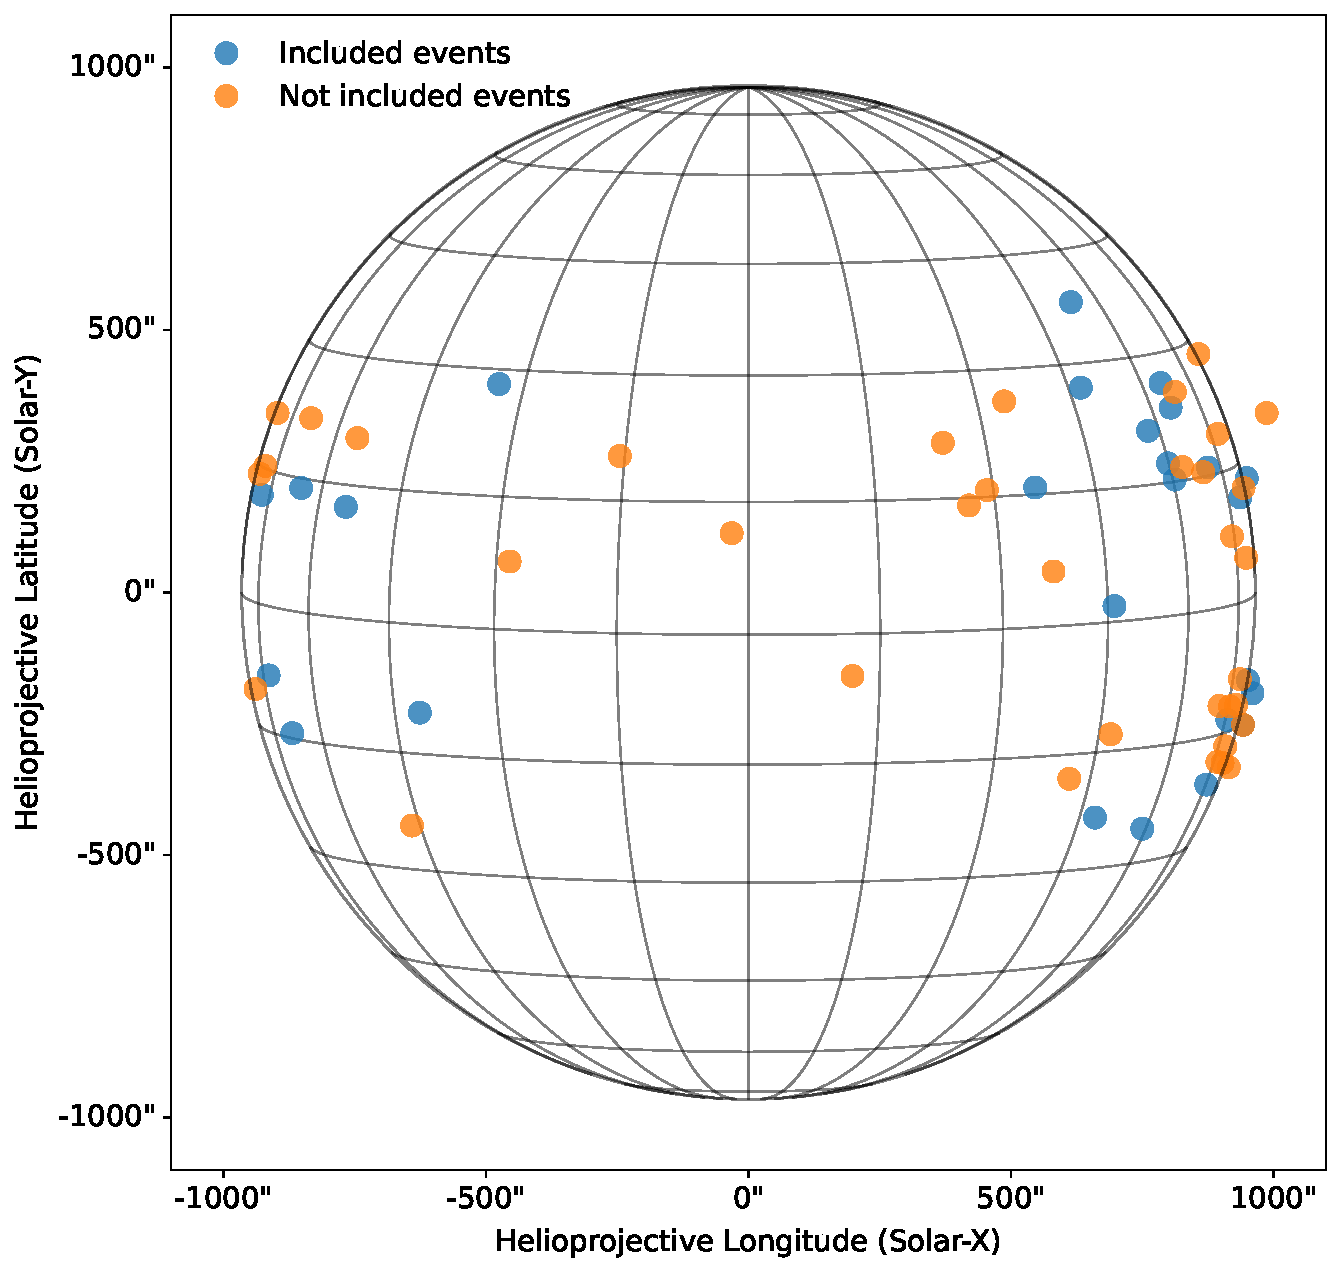
\includegraphics[width=0.7\columnwidth]{chapter2/figs/events_coords.pdf}}
	\caption{Distribution of the source location of the CBFs on the solar disk. The blue dots are the events that we included in Table~\ref{table_1}, while the orange dots are the events that we did not include in the table.}
	\label{fig_solardisk}
\end{figure}

The kinematics are determined through time-height maps, commonly known as J-maps \citep{sheeley_1999}. These maps are generated by stacking columns of pixels in a desired direction from a solar image. The track's shape on J-maps depends on the feature's direction and speed, allowing identification of radial and lateral wave front positions over time. 

Our analysis approximates radial and lateral wavefront positions using J-maps generated for each event. Assuming symmetrical expansion on both flanks, we treat the waves as spheroids defined by major and minor axes. Consequently, the radial direction is represented by a single value, while the lateral direction (parallel to the solar limb) uses two values for measurements in both left and right directions. However, lateral wave signatures may sometimes be visible in only one direction or be absent entirely.
Due to data limitations, our final sample size is 26 events, prioritizing complete datasets that exclude events with missing radial, lateral, or combined measurements.

To extract relevant plasma parameters and perform modeling, we retrieve information on CBFs from the HEK database and consult Nariaki Nitta's catalog of coronal waves  \citep{nitta_2013}\footnote{Nariaki Nitta's Catalog: \url{https://lmsal.com/nitta/movies/AIA_Waves/index.html}} to obtain necessary data. With the event list, we employ the SPREAdFAST framework to calculate kinematics, infer shock parameters, and determine plasma properties. Detailed summary plots of the modeled events can be found on the online SPREAdFAST catalog\footnote{SPREAdFAST Catalog: \url{https://spreadfast.astro.bas.bg/catalog/}}.

\begin{figure}[!htp] % updated!
	\centerline{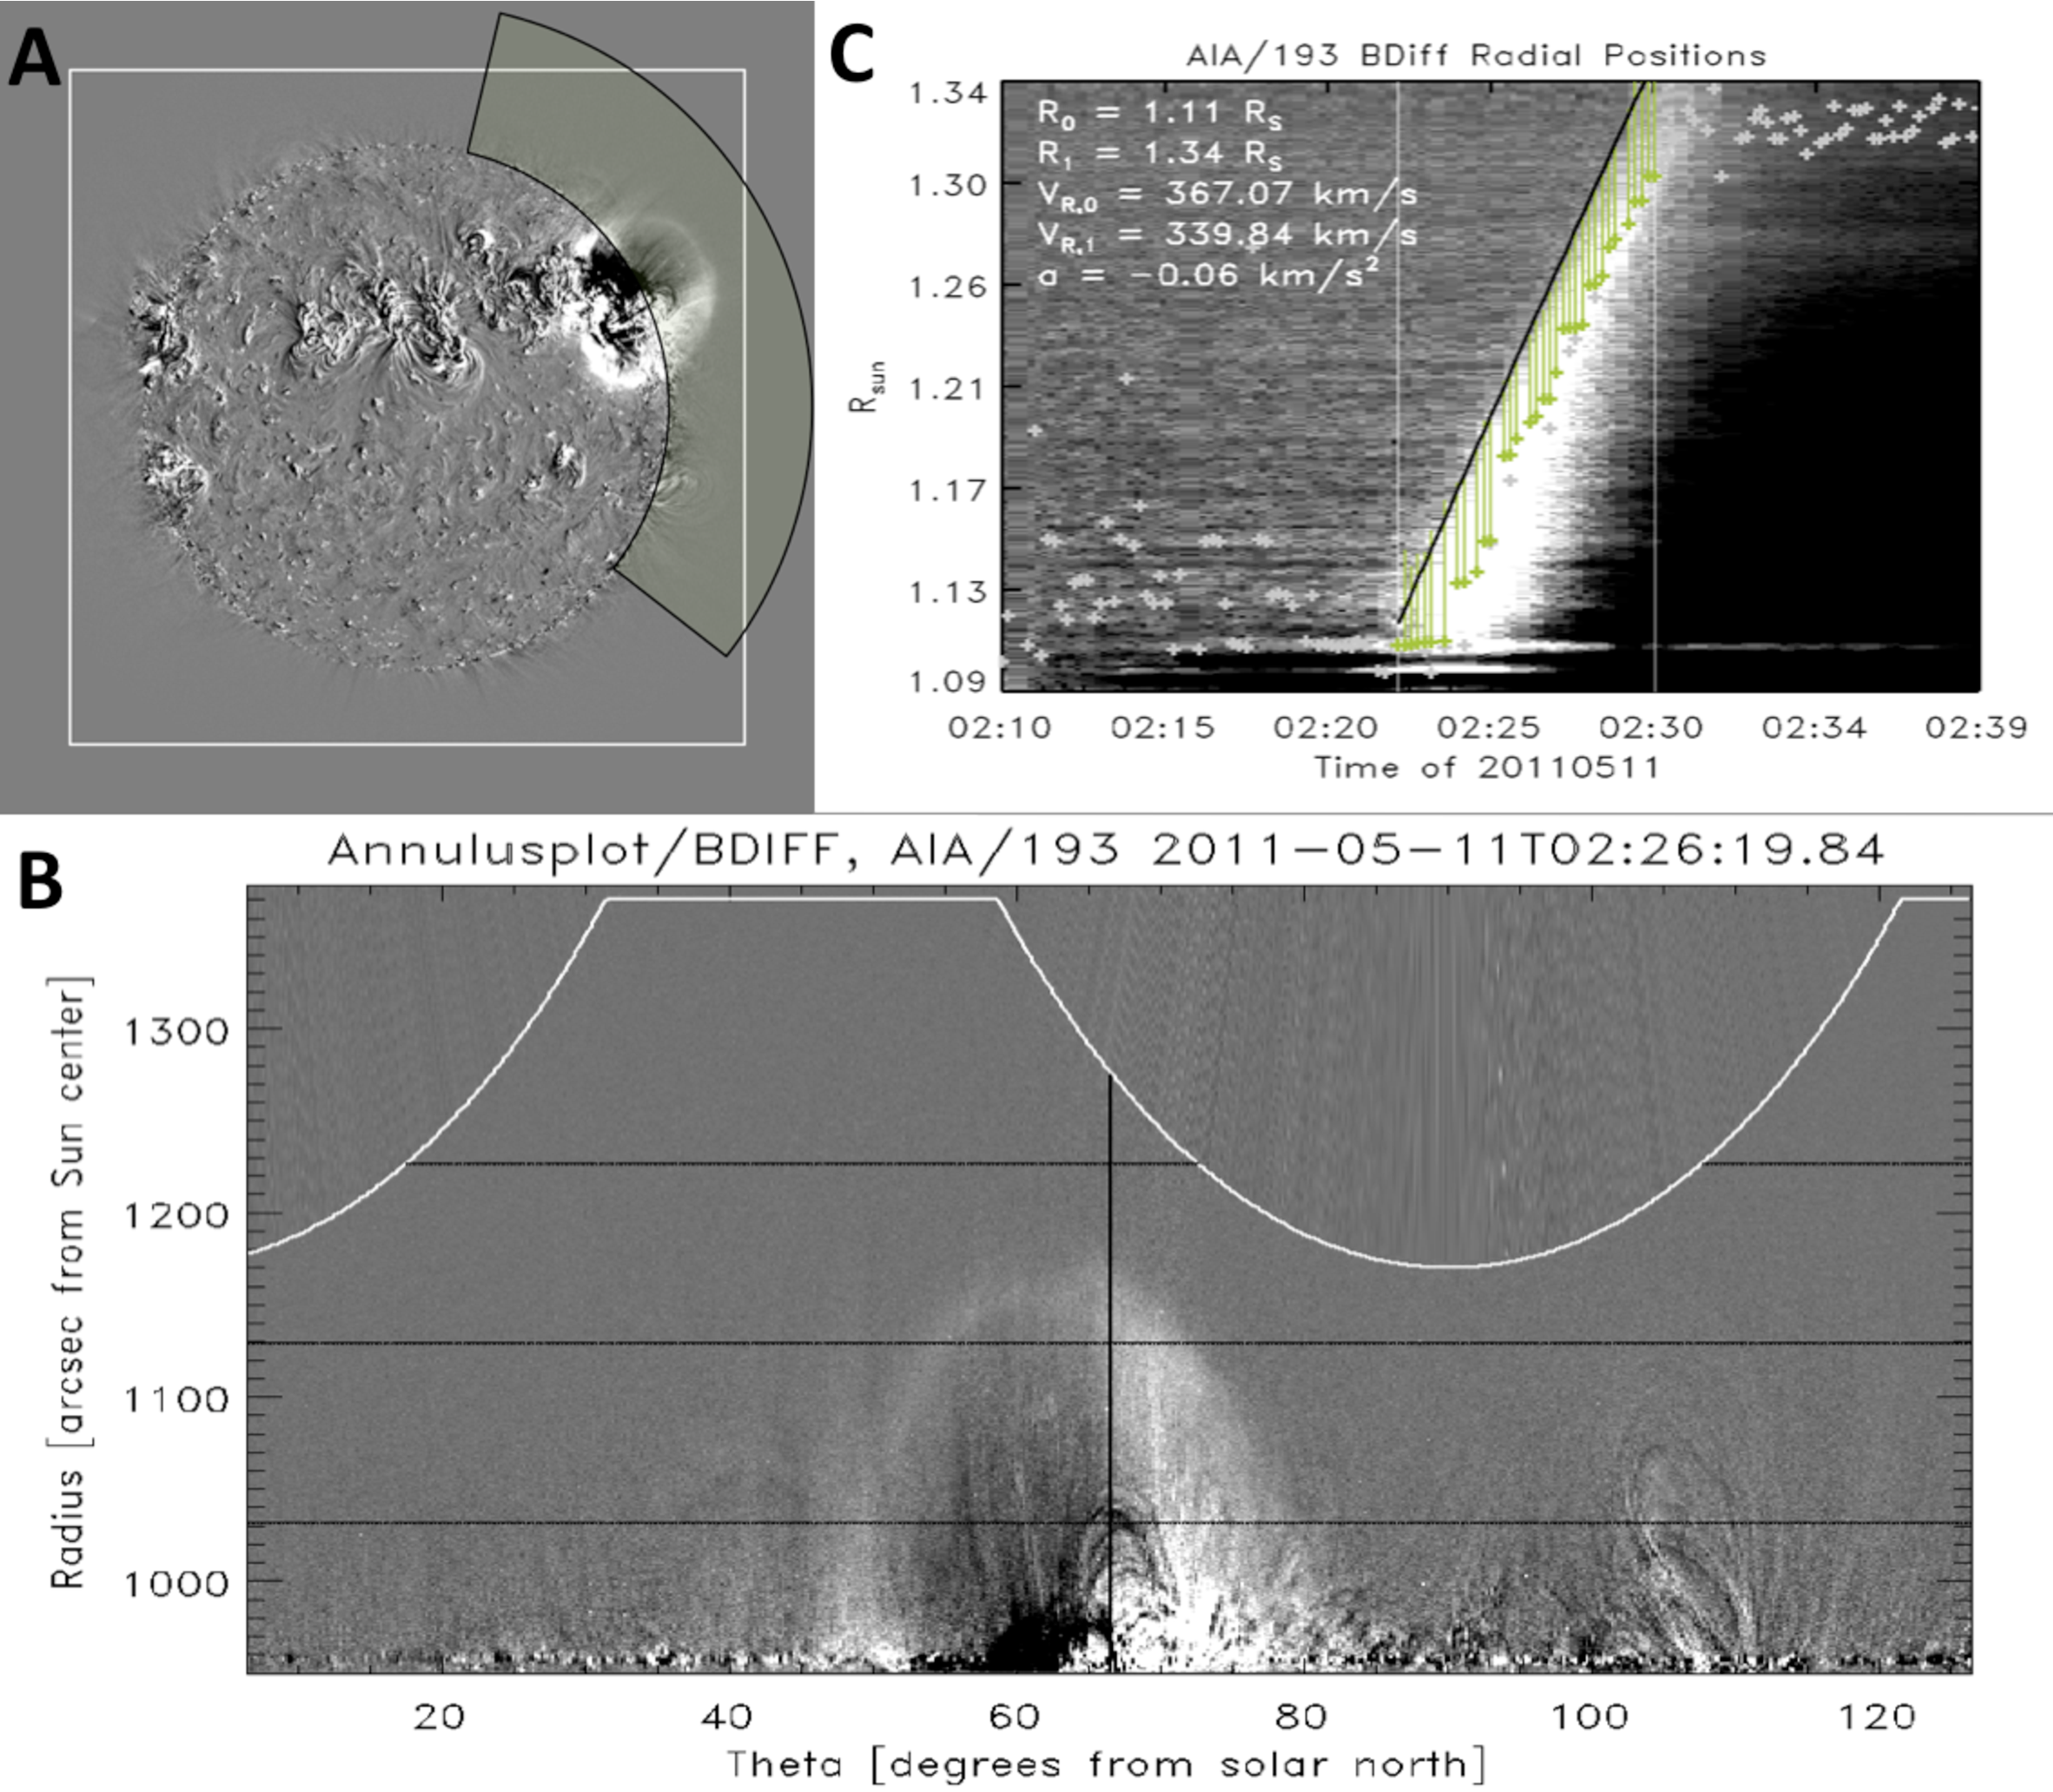
\includegraphics[width=0.9\columnwidth]{chapter2/figs/fig_annplot.pdf}}
	\caption{Illustration for the annulus method used to extract kinematic data from AIA images. (A) shows the full Sun disk with the relevant region highlighted for analysis (green sector). The white box outlines the AIA FOV. (B) displays the extracted annular region mapped onto polar coordinates, with the actual data extent marked by the white curve. Black lines indicate the directions used for measuring radial and lateral motions. (C) shows a stacked plot of intensity along the radial direction, with green markers highlighting intensity peaks and their corresponding distances from the CBF wavefront. The white lines represent the time interval during which the CBF is tracked within the AIA FOV. This figure is curated from \citep{kozarev_2017}.}
	\label{fig_annplot}
\end{figure}

To accurately determine the front, back, and peak of the EUV wave at each time step (Fig.~\ref{fig_jmaps_110511}), we applied several algorithms. Firstly, we utilized Savitzky-Golay filtering \citep{savitzky_1964} to smoothen the data. Next, we employed local minima/maxima ordering and proximity/intensity metrics algorithms. These algorithms enabled us to identify the wave positions and extract relevant parameters.
For each CBF event, we manually specified the starting and ending times, indicated by vertical white lines in Figure~\ref{fig_jmaps_110511}. We also determined the starting and ending height, corresponding to the off-limb portion of the CBF within the AIA FOV.

\begin{figure}[!htp] % updated!
	\centerline{
		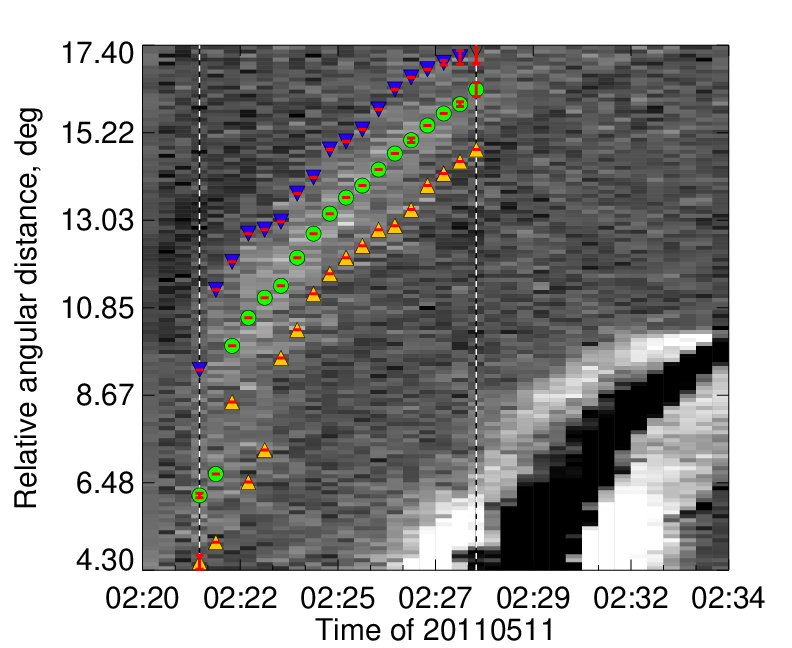
\includegraphics[width=0.32\textwidth,clip=]{chapter2/figs/avg_wave_lat_pos_110511_01_r1_left.png}
		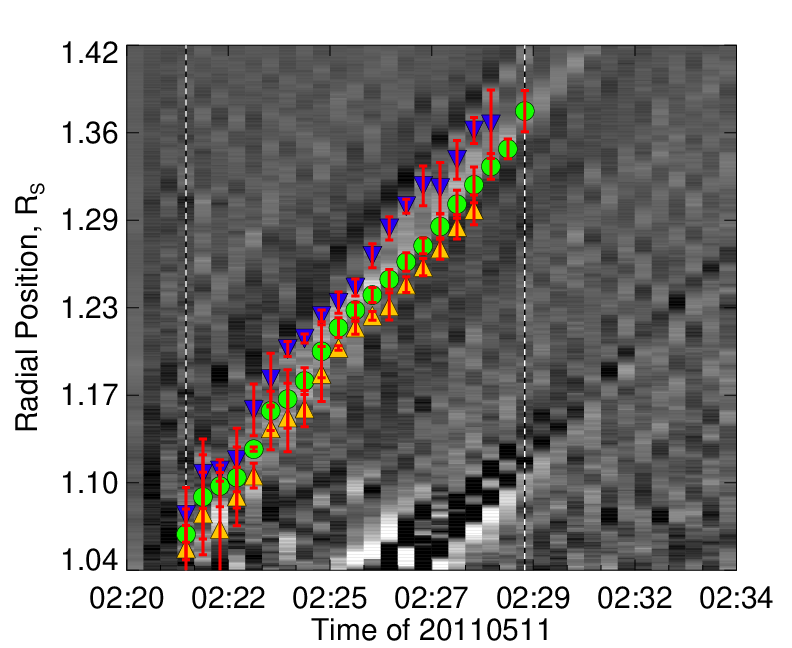
\includegraphics[width=0.32\textwidth,clip=]{chapter2/figs/avg_wave_rad_pos_110511_01.png}
		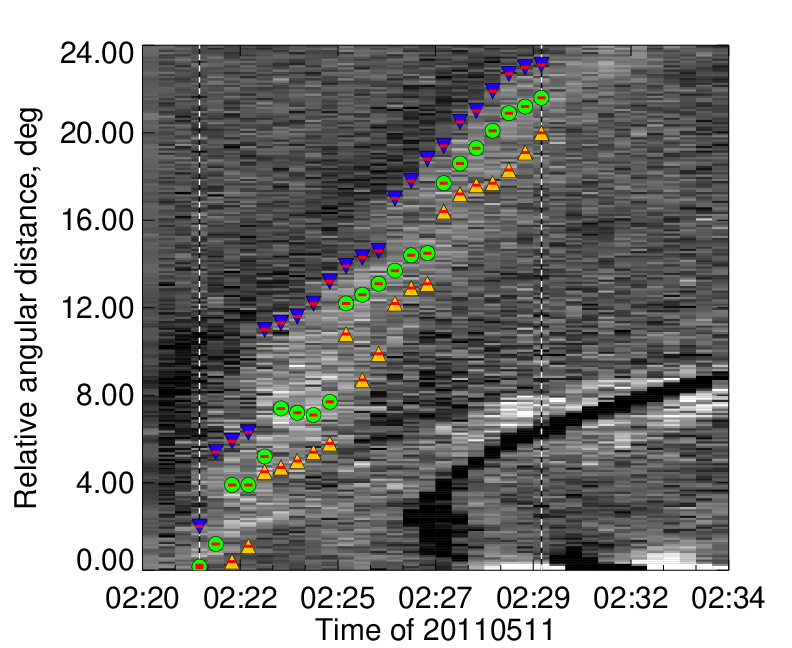
\includegraphics[width=0.32\textwidth,clip=]{chapter2/figs/avg_wave_lat_pos_110511_01_r1_right.png}
	}
	\caption{J-map plots for the event of May 11, 2011, for the radial direction (middle plot) and the left and right flanks of the wave in the lateral heliocentric direction (the left and right plots, respectively). Blue, green, and orange filled symbols are the positions of the CBF front, peak, and back, respectively. The uncertainty of the average measurements is shown as red bars.}
	\label{fig_jmaps_110511}
\end{figure}

By analyzing the intensity values, we defined the CBF positions as the locations with peak intensity at each time step. The front and back of the wave were set at 20\% of the peak intensity.
To obtain more comprehensive information about the CBFs, we applied the Levenberg-Marquardt least squares minimization \citep{markwardt_2009} along with a second-degree bootstrapping optimization technique \citep{efron_1979}. This approach allowed us to fit fourth-order polynomials to the wave positions using Savitzky-Golay fitting. As a result, we obtained measurements for speeds, accelerations, intensities, and thicknesses of the waves in both the radial and lateral directions. The thicknesses and intensities are averages of the values between the peak and back for each time step. Measurements of the heights of CBFs with respect to the solar disk center were obtained\footnote{LASCO CME Catalog: \url{https://cdaw.gsfc.nasa.gov/CME_list/}} for all the events analyzed in this study. These measurements were taken at the fastest segment of the leading edge of each CBFs over time.
We also have measurements of the lateral positions of the CBF front relative to the nose direction. These were obtained in degrees and converted to km depending on the height of the lateral measurement above the solar surface.

\section{Data Analysis and Methods}

%\subsection{The SPREAdFAST Framework}
%The Solar Particle Radiation Environment Analysis and Forecasting-Acceleration and Scattering Transport (SPREAdFAST) framework is a physics-based global modeling framework integrates detailed Extreme Ultraviolet (EUV) observations of Coronal Mass Ejection-driven Shock and Sheath (CBF) events with modeling of the interacting coronal plasma and the subsequent production and interplanetary transport of Solar Energetic Particles (SEPs). The following sections provide a concise overview of the key components utilized in the SPREAdFAST framework for this study.

\subsection{Modeling}
The Solar Particle Radiation Environment Analysis and Forecasting–Acceleration and Scattering Transport \citep[SPREAdFAST]{kozarev_2022} is a physics-based prototype heliospheric SEP forecasting system. It incorporates data-driven models to estimate the coronal magnetic field, dynamics of coronal shock waves, energetic particle acceleration, and scatter-based SEP propagation in the heliosphere. The system is based on the Coronal Analysis of SHocks and Waves framework \citep[CASHeW]{kozarev_2017} and provides timely predictions of SEP arrival times, maximum intensities, and SEP fluxes at various locations in the inner heliosphere. It contributes to space weather requirements, protecting ESA assets, aiding satellite operators, and providing lead times for mitigating impacts on electronics and humans in space activities.

%To extract relevant plasma parameters and perform modeling for the events, our approach involves several steps. First, we retrieve information on coronal wave events from the HEK database\footnote{HEK Database: \url{https://www.lmsal.com/isolsearch}}. Additionally, we consult Nitta's catalog\footnote{Nitta's Catalog: \url{https://lmsal.com/nitta/movies/AIA_Waves/index.html}} of coronal waves \citep{nitta_2013}. These sources provide us with the necessary data to proceed.

%Once we have the event list, we employ the SPREAdFAST framework to calculate kinematics, infer shock parameters, and determine plasma properties. Detailed summary plots of the modeled events can be found on the online SPREAdFAST catalog\footnote{SPREAdFAST Catalog: \url{https://spreadfast.astro.bas.bg/catalog/}}.

%In our analysis, we approximate the radial and lateral wavefront positions over time using J-maps generated with the CASHeW code for each event. To simplify the modeling process, we assume symmetrical expansion of the waves on both sides, treating them as spheroids defined by major and minor axes. Consequently, we represent the radial direction with a single value and the lateral direction (i.e. parallel to the solar limb) with two values, considering measurements in two directions away from the radial direction. However, it is worth noting that lateral wave signatures may sometimes be visible in only one direction or absent entirely. Summary plots of the J-maps, including estimated positions and errors, can be found in the online SPREAdFAST catalog for each event. To create a unified lateral kinematics time series for each event, we average measurements from both lateral flanks. Additionally, we record the CBF mean intensity and thickness in both directions.
%To analyze the kinematic measurements deduced from the AIA FOV, we apply a Savitzky-Golay fit \citep{savitzky_1964}, as described in \citet{kozarev_2019}. Subsequently, we extrapolate the smoothed radial positions up to \almost17\rsun using the analytical CME kinematics models presented by \citet{gallagher_2003} and \citet{byrne_2013}.

Summary plots of the J-maps, including estimated positions and errors, can be found in the online SPREAdFAST catalog for each event. To create a unified lateral kinematics time series for each event, we average measurements from both lateral flanks. Additionally, we record the CBF mean intensity and thickness in both directions.
To analyze the kinematic measurements deduced from the AIA FOV, we apply a Savitzky-Golay fit \citep{savitzky_1964}, as described in \citet{kozarev_2019}. Subsequently, we extrapolate the smoothed radial positions up to $\sim$17\rsun using the analytical CME kinematics models presented by \citet{gallagher_2003} and \citet{byrne_2013}.

Our next step involves developing multiple synthetic geometric shock models, known as the synthetic shock model (S2M) module, to describe the shock surface at a 24-second cadence. These models rely on extrapolated radial and lateral kinematic results, as well as the inferred major and minor axes of the spheroids representing compressive waves. The shock surface is created from the onset of the CBF until its nose reaches 10\rsun and is then propagated up to $\sim$17\rsun. The propagation is based on the Magnetohydrodynamic Algorithm outside a Sphere (MAS) synoptic coronal MHD model's results. Consequently, the shock surface samples plasma parameters from the data cube of the MAS model at discrete points, determined by consecutively crossing magnetic field lines.
The MHD data utilized in this study is represented as a 3D data cube consisting of plasma parameters. To analyze this data, a spheroid model was propagated through the data cube by scanning it without any direct interaction. At each point within the data cube, a search was conducted to identify the nearest four neighbors. By employing trilinear interpolation, the values at these points were estimated.

By sampling the shock surface, we obtain data for approximately 1000 field-crossing lines, potentially more depending on the desired resolution. For each event, the output consists of a set of data structures that describe each shock-crossing field line. These structures include the shock speed $V_{shock}$, plasma density $n$, density jump $r$, shock upstream magnetic field magnitude $B_{mag}$, shock-field angle $\theta_{BN}$, Alfven speed $V_A$, and Alfven Mach number $M_A$.

To estimate the shock density jump, we follow the method of \citet{kozarev_2017} - we calculate the differential emission measure (DEM) before and during the event at each shock crossing and each timestep. The DEM is obtained using the model by \citet{cheung_2015}. We integrate the DEM to obtain the average density, and take the ratio of densities during and before the event.
Typically, the density jump within the AIA FOV is relatively small, usually below 1.2. However, beyond this region where observational information is lacking, we assign a value of 1.2, assuming a weak shock.
For ease of analysis, we divide the synthetic shock model into three segments: the cap (representing the shock nose), Zone 1, and Zone 2 (referring to the shock flanks). This division allows us to examine the distribution of plasma parameters across different sectors of the shock surface. Figure~\ref{fig_segments} illustrates the evolution of the synthetic shock model in nine timesteps, with the cap zone colored blue and the shock flanks colored green and red.

\begin{figure}[!htp] % updated!
	\centerline{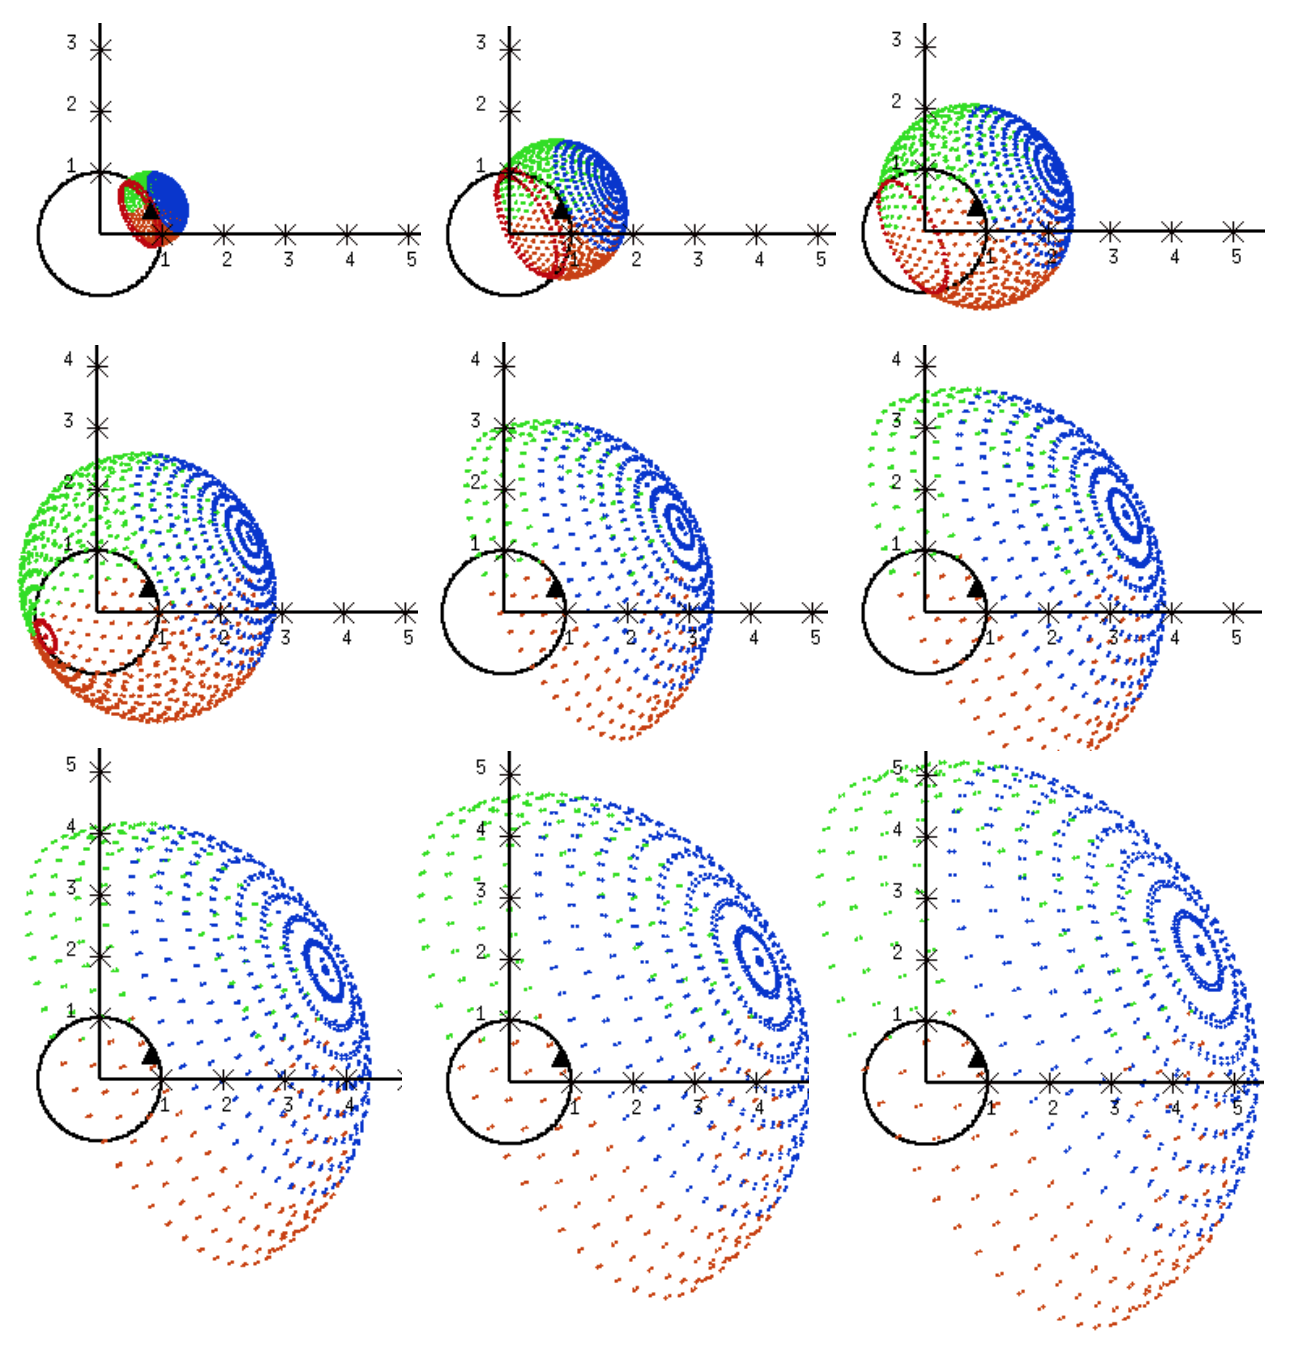
\includegraphics[width=0.7\columnwidth]{chapter2/figs/fig_s2m_segments_geometry.png}}
	\caption{Synthetic shock model divided into three segments; the cap zone in blue and the flank zones are in red and green.}
	\label{fig_segments}
\end{figure}

\section{CBF Kinematics and Geometric Modeling - Case Study May 11, 2011}
In this section, we provide a detailed analysis of the event at the low corona region, demonstrating our method. Additionally, we investigate the plasma parameters along individual shock-crossing magnetic field lines in the AIA FOV.

\subsection{Event Context}
The eruption took place on May 11, 2011, at approximately 02:20 UT (Fig.~\ref{fig_aia_event}). It originated from an active region situated in the northwestern sector (N18W52). The event involved a massive shock wave propelled by a fast partial-halo CME that occurred at 02:48 UT. The CME exhibited a linear speed of 745 \kms, a 2$^{nd}$-order speed at 20\rsun of 776 \kms, an acceleration of 3.3 m s$^{-2}$, an angular width (AW) of 225\degree, a central position angle (PA) of 320\degree, a measurement position angle (MPA) of 283\degree, a mass of 3.5$\times$10$^{15}$ gram, and a kinetic energy of 9.6$\times$10$^{30}$ erg. The mass and kinetic energy were uncertain due to projection effects, as reported by the SOHO-LASCO CME catalog. This was accompanied by a weak solar flare classified as B8.1 and an eruptive filament, as observed by the 193 $\AA$ EUV channel of the SDO/AIA.

\begin{figure}[!htp] % updated!
	\centerline{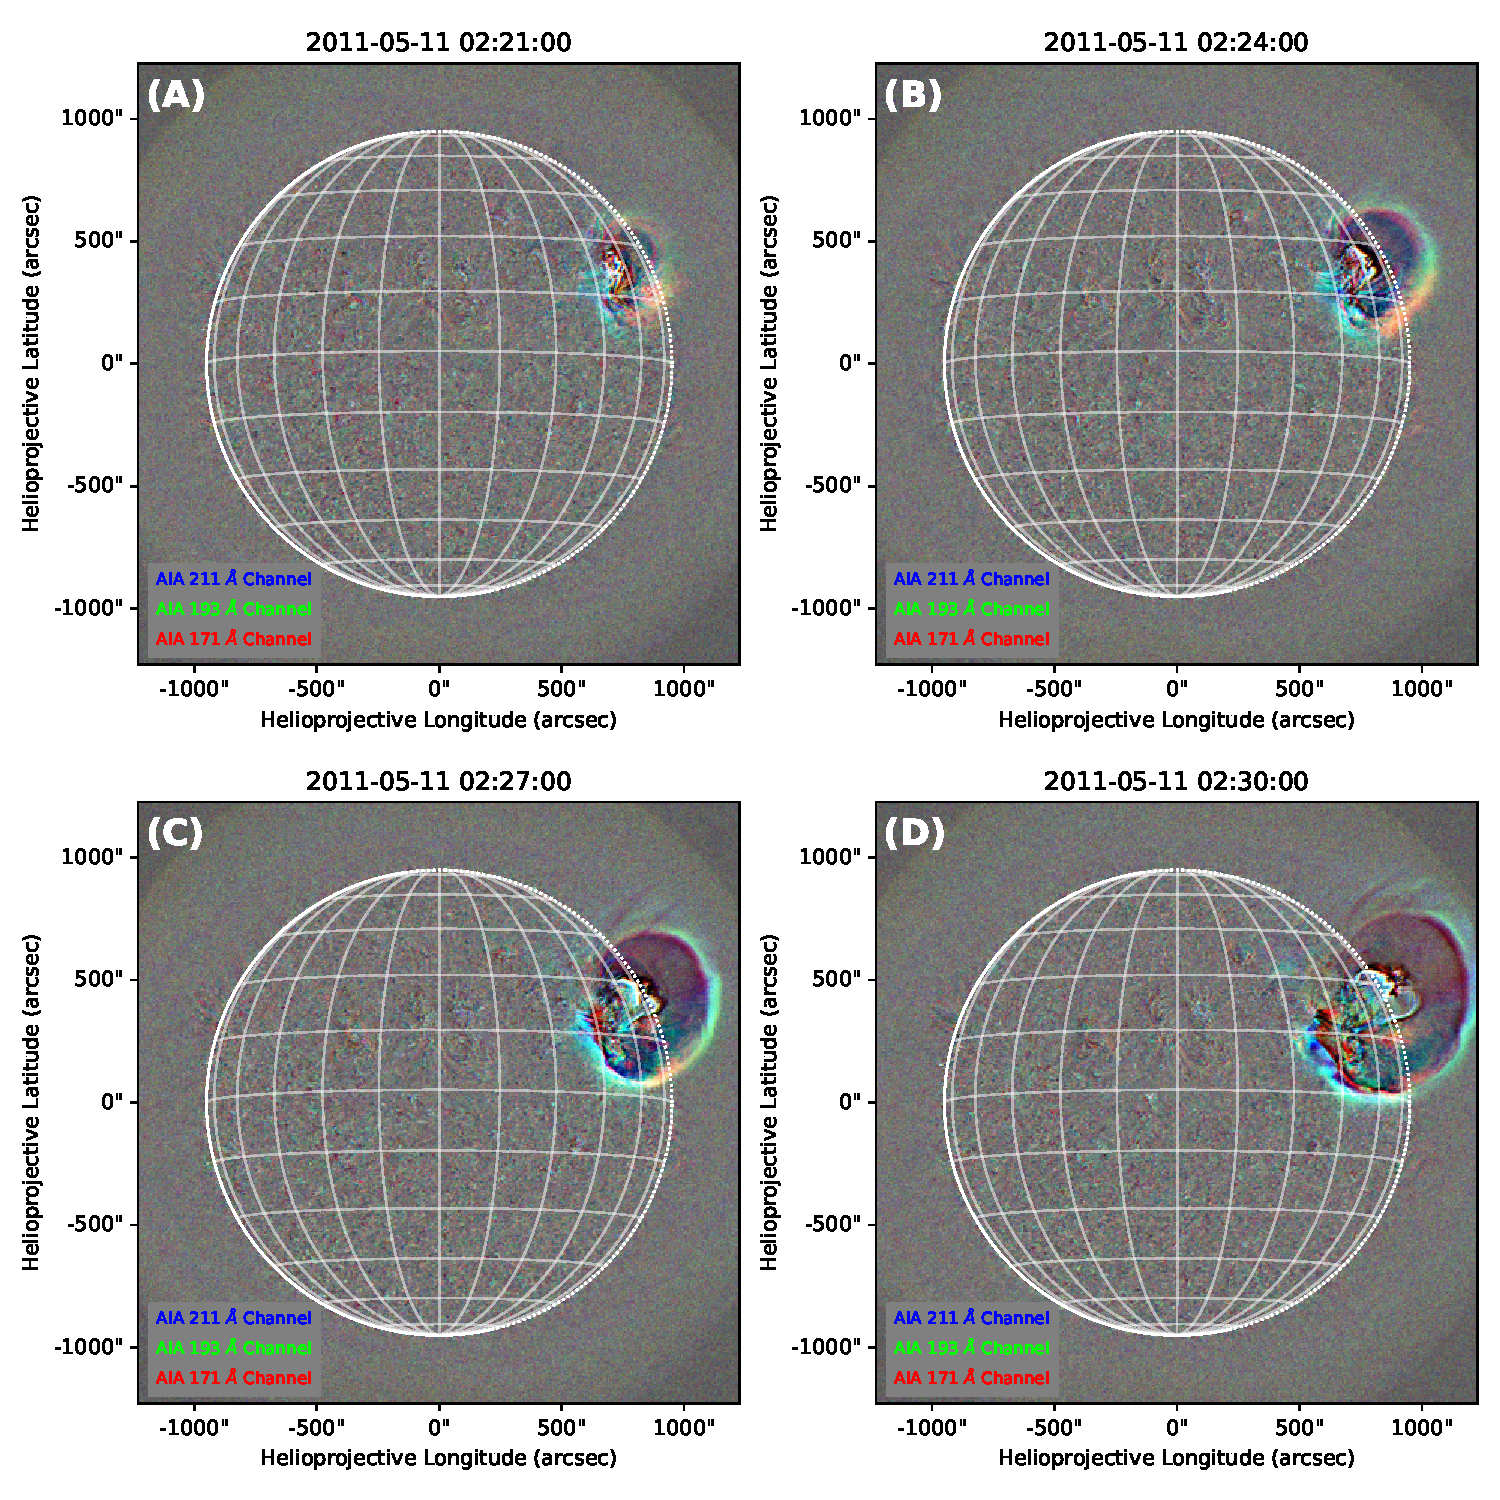
\includegraphics[width=0.8\columnwidth]{chapter2/figs/RGB_panel.pdf}}
	\caption{AIA running-difference images capture a coronal wave evolving over 9 minutes near the Sun's western limb, exhibiting markedly changing intensity and structure as observed in 171, 193, and 211 $\AA$.}
	\label{fig_aia_event}
\end{figure}

Furthermore, the eruption was associated with a type II radio burst, which commenced around 02:20 UT. This was observed by the Learmonth spectrogram (25-180 MHz) maintained by the Australian Space Weather Services and part of the CALLISTO global network. By examining the OMNI database\footnote{OMNIWeb Database: \url{https://omniweb.gsfc.nasa.gov/}}, we found no evidence of a geomagnetic storm occurring within three days from the onset of the eruption. Nevertheless, an increase in proton fluxes across all energy channels near 1 AU was observed using the SOHO/ERNE instrument. According to the Wind/EPACT catalog\footnote{Wind/EPACT Catalog: \url{http://newserver.stil.bas.bg/SEPcatalog/}} \citep{miteva_2016, miteva_2017}, we found an SEP event detected by the SOHO/ERNE instrument at the Earth with onset time of 03:39 UT and a $J_p$ of 0.0133 protons/(cm$^2$ s sr MeV) in the energy channel 17-22 MeV. $J_p$ is the peak proton intensity after subtracting the pre-event level.

\subsection{Low Corona Part}
To investigate the kinematics of the CBF event, we employed the CASHeW module within the SPREAdFAST framework. As we see in Figure~\ref{fig_jmaps_110511}, the J-maps are displayed, illustrating the radial and lateral time-dependent evolution of the CBF in gray-scale. Since the wave is assumed to have a dome-like shape, the lateral direction is divided into left and right flanks. Bright features below the CBF in the J-maps are likely expanding loops. To estimate the uncertainty in the measurements, we varied slightly the radial (nose) direction three times. The corresponding positions are depicted in red, while the start and end times of the CBF are indicated by vertical dashed lines. Additionally, the front, back, and peak of the CBF are represented by blue down-pointing triangles, yellow up-pointing triangles, and green-filled circles, respectively.

Figure~\ref{fig_kinematics_110511} presents the time series kinematic results of the shock wave parameters within the SDO/AIA field of view (up to 1.3\rsun). The kinetics of the wavefront, peak, and back are color-coded as red, green, and blue, respectively. The subpanels from top to bottom display the estimated heliocentric distance, speed, acceleration, intensity, and thickness of the wave. These parameters are presented for both the radial (middle panel) and lateral directions (left and right panels).

\begin{figure}[!htp] % updated!
	\centerline{
		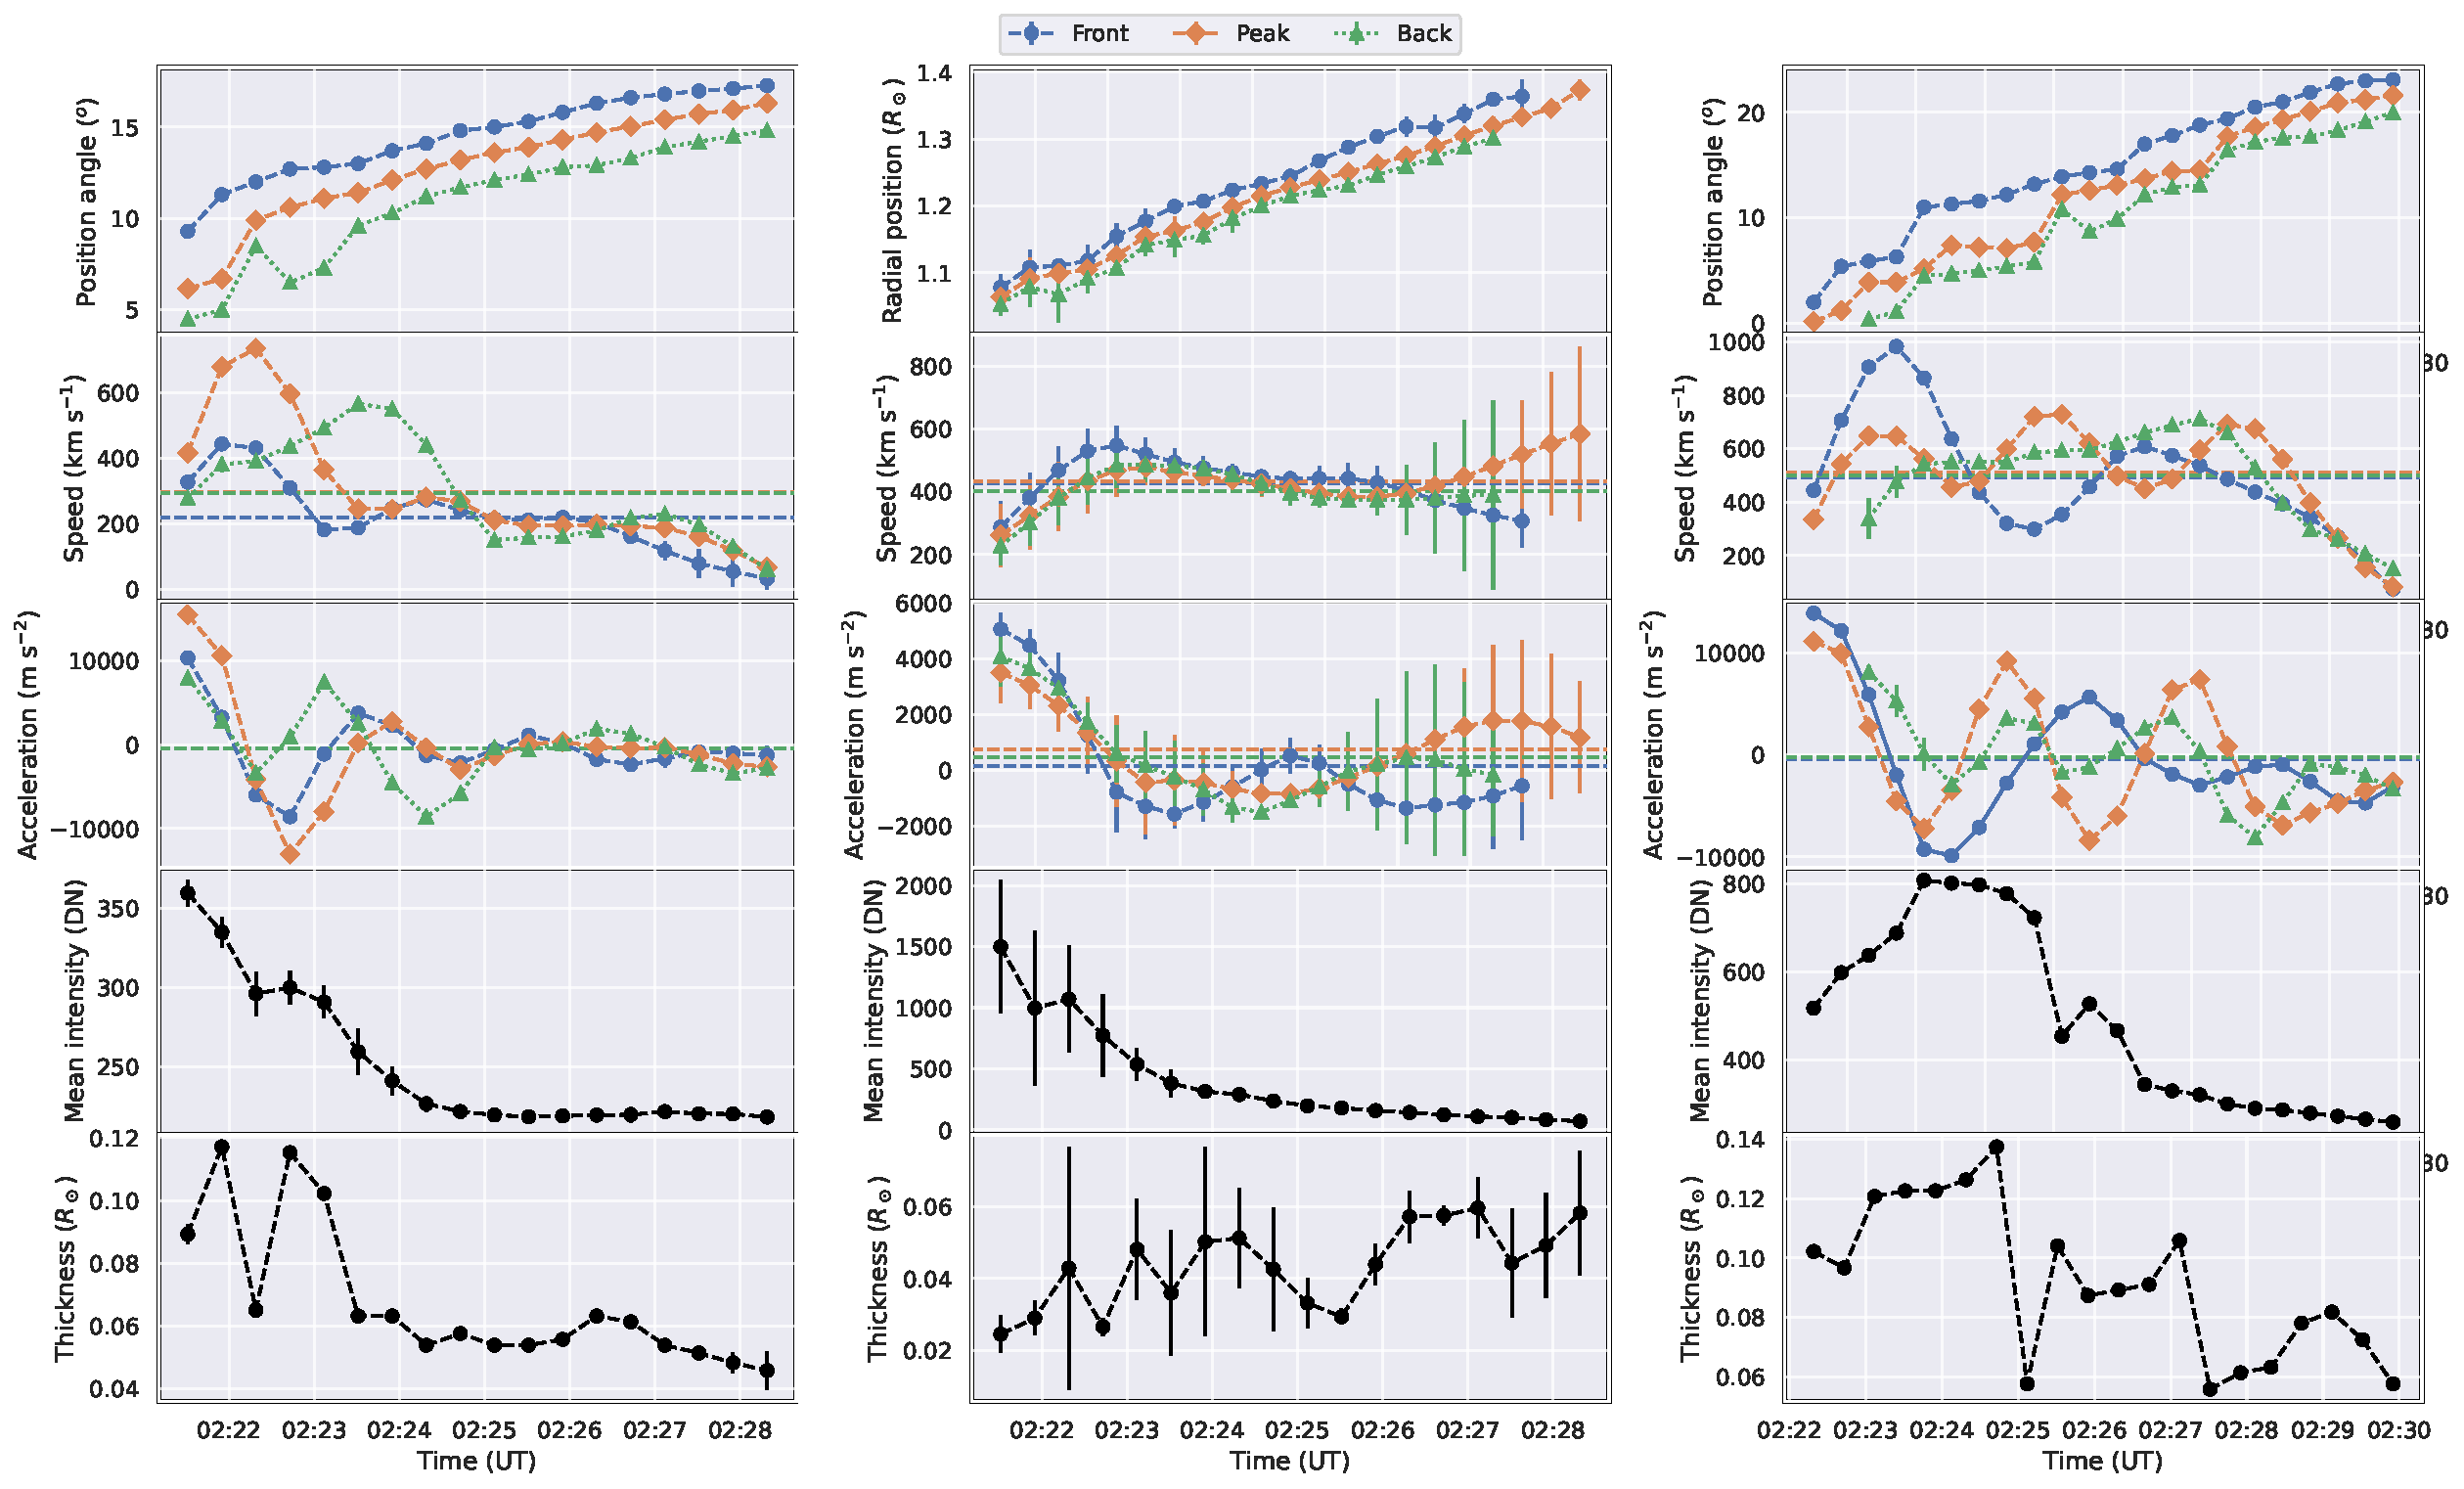
\includegraphics[width=1\textwidth,clip=]{chapter2/figs/euvwave_kinematics_110511_01.pdf}
	}
	\caption{Time-series kinematics of the CBF parameters for the front, peak, and back positions in the AIA FOV, with measurement uncertainties shown as small bars over the data points. The horizontal lines in the speed and acceleration panels denote the mean speeds and accelerations for the wave front, peak, and back with respective colors. The left and right columns represent the lateral kinematic measurements in the left and right flanks of the wave, respectively. The middle column represent the kinematic measurements in the radial direction.}
	\label{fig_kinematics_110511}
\end{figure}

Analysis of Figures~\ref{fig_jmaps_110511} and~\ref{fig_kinematics_110511} reveals that the coronal wave was asymmetric in shape. The time-dependent evolution of the angular distance differed slightly between the left and right flanks. In Figure~\ref{fig_jmaps_110511}, the right flank (towards the solar equator) of the wave appeared for a little bit longer time, allowing the algorithm to capture it with a higher number of measurements until approximately 02:29 UT, same as for the radial direction. In contrast, the left flank (towards the solar pole) had fewer measurements available.

The coronal wave's initial appearance was slightly elongated, with an aspect ratio of 0.5. This indicates a longer major axis, creating a degree of asymmetry. At 02:25:31 UT, a striking change occurred: the wave became perfectly circular, achieving an aspect ratio of 1. This signifies equal lengths for both axes, resulting in a symmetrical shape. However, this transformation was short-lived. The wave's morphology shifted again, becoming increasingly flattened. This signifies a growing minor axis compared to the major one, leading to an \textit{over-expansion} of the wave along its minor axis.
In this study, the aspect ratio is defined as the minor axis divided by the major axis of the wave's geometric surface. A value of 1 represents a perfectly symmetrical wave, while values greater than 1 indicate over-expansion along the minor axis. Conversely, values less than 1 point towards elongation along the major axis, reflecting a more radial expansion.

Regarding the radial direction, the event duration spanned from approximately 02:21 to 02:28 UT. The shock wave exhibited an average speed of approximately 420.46 \kms, while the average acceleration was around 463.92 m s$^{-2}$, calculated as the mean of the front, peak, and back sides of the wave. For the left flank in the lateral direction, the event duration spanned from around 02:21 to 02:28 UT. The average speed and acceleration were approximately 270 \kms and -400.62 m s$^{-2}$, respectively. For the right flank in the lateral direction, the event duration spanned from around 02:21 to 02:30 UT, lasting for one minute longer than the left flank. The average speed and acceleration were approximately 500.97 \kms and -297.18 m s$^{-2}$, respectively.

Comparing the lateral directions, the wave's sheath on the right flank was approximately six times the thickness observed on the left flank, while the radial direction exhibited a thickness roughly half that of the left flank. Notably, the peak speed in the radial direction was lower than that in the lateral direction; right flank, suggesting that the shock wave experienced compression in the direction of propagation, while expanding laterally to a greater extent than radially. Table~\ref{T_110511} provides a summary of the statistical results.

To further explore the shock and plasma parameters at different sections of the coronal wave, we divided the shock surface into three segments: the Cap zone (shock nose), Zone 1, and Zone 2 (the shock flanks). This division is illustrated in Figure~\ref{fig_segments}.

\begin{table}[!htp] % updated!
	\centering
	\caption{Mean values and their standard deviation of the wave parameters in the radial direction and the lateral direction for the left and right flanks, at the front, peak, and back sides of the wave for the event occurred on May 11, 2011, in the SDO/AIA FOV.}
	\label{T_110511}
	\resizebox{\textwidth}{!}{%
		\begin{tabular}{lc|c|c|c}
			\hline
			Parameter                              & Direction  & Front              & Peak                   & Back                 \\ \hline
			\multirow{3}{*}{$<speed>$ \kms}        & Lat. Left  & 218.46 $\pm$ 9.04  & 297.46 $\pm$ 5.45      & 293.94 $\pm$ 9.04    \\ \cline{2-5}
			& Radial     & 427.46 $\pm$ 51.85 & 433.11 $\pm$ 82.86     & 400.81 $\pm$ 83.78   \\ \cline{2-5} 
			& Lat. Right & 494.69 $\pm$ 0.00  & 509.25 $\pm$ 1.02      & 498.97 $\pm$ 9.21    \\ \hline
			\multirow{3}{*}{$<accel.>$ m s$^{-2}$} & Lat. Left  & -414.62 $\pm$ 227.23 & -401.46 $\pm$ 164.62 & -385.77 $\pm$ 227.23 \\ \cline{2-5}
			& Radial     & 147.41 $\pm$ 1009.19 & 758.97 $\pm$ 1287.65 & 485.38 $\pm$ 1365.80 \\ \cline{2-5} 
			& Lat. Right & -415.04 $\pm$ 0.00   & -209.81 $\pm$ 22.32  & -266.68 $\pm$ 250.80 \\ \hline
			\multirow{3}{*}{$<intensity>$ DN}      & Lat. Left  & \multicolumn{3}{c}{250.60 $\pm$ 5.90}               \\ \cline{2-5}
			& Radial     & \multicolumn{3}{c}{403.34 $\pm$ 143.30}             \\ \cline{2-5}
			& Lat. Right & \multicolumn{3}{c}{489.04 $\pm$ 2.86}               \\ \hline
			\multirow{3}{*}{$<thickness>$\rsun}   & Lat. Left  & \multicolumn{3}{c}{0.07 $\pm$ 0.00}                 \\ \cline{2-5}
			& Radial     & \multicolumn{3}{c}{0.04 $\pm$ 0.01}                 \\ \cline{2-5}
			& Lat. Right & \multicolumn{3}{c}{0.09 $\pm$ 0.00}                 \\ \hline
		\end{tabular}%
	}
\end{table}

\begin{table}[!htp] % updated!
	\centering
	\caption{Mean, median, and standard deviation of the shock parameters output, from the interaction of the S2M spheroid with the MAS MHD model results, for the shock's cap and flanks and for the whole shock surface, for the event on May 11, 2011.}
	\label{T_sh_param_110511}
	\begin{tabular}{lcccc}
		\hline
		\multirow{2}{*}{Segment} & \multirow{2}{*}{Parameter} & \multicolumn{3}{c}{Statistics} \\
		&                         & Mean & Median & Stdv \\ \hline
		All & $V_{SHOCK}$ \kms    & 577.77 & 578.39 & 72.79 \\ 
		& $\theta_{BN}$ \degree   & 70.06 & 0.63 & 44.83 \\ 
		& $B_{MAG}$ G             & 0.046 & 0.038 & 0.070 \\ 
		& Density Jump            & 1.193 & 1.188 & 0.185 \\ \hline
		
		Cap & $V_{SHOCK}$ \kms    & 555.18 & 550.86 & 42.46 \\ 
		& $\theta_{BN}$ \degree   & 19.37 & 3.61 & 25.51 \\ 
		& $B_{MAG}$ G             & 0.046 & 0.036 & 0.070 \\ 
		& Density Jump            & 1.193 & 1.188 & 0.015 \\ \hline
		
		Zone 1 & $V_{SHOCK}$ \kms & 613.69 & 609.32 & 59.42 \\ 
		& $\theta_{BN}$ \degree   & 6.46 & 0.21 & 50.92 \\ 
		& $B_{MAG}$ G             & 0.045 & 0.045 & 0.066 \\ 
		& Density Jump            & 1.190 & 1.187 & 0.008 \\ \hline
		
		Zone 2 & $V_{SHOCK}$ \kms & 631.37 & 614.23 & 73.07 \\ 
		& $\theta_{BN}$ \degree   & 0.10 & 0.51 & 10.61 \\ 
		& $B_{MAG}$ G             & 0.046 & 0.029 & 0.071 \\ 
		& Density Jump            & 1.194 & 1.188 & 0.016 \\ \hline
	\end{tabular}
\end{table}

We summarize the results for the three segments in Table~\ref{T_sh_param_110511} to further investigate the shock and plasma parameters in different sections of the coronal wave. Notably, the mean shock speed at the flanks was higher than that at the Cap zone. We did not observe significant variations in the magnetic field across the different segments, indicating a relatively homogeneous magnetic structure. The shock density jump exhibited consistent values across all three segments.

In \citet{kozarev_2022} we investigated shock-crossing magnetic field lines during this event, and key plasma parameters were analyzed up to 10\rsun. The study, utilizing DEM analysis, revealed consistent results with weak coronal shocks. Notably, the density jump within the AIA FOV was generally small, below 1.2, aligning with previous research. Beyond this view, lacking observational data, the density jump was set to 1.2.
By inspecting the parameter evolution over all shock-crossing field lines, we found that the shock-field angle ($\theta_{BN}$) and magnetic field amplitude ($|B|$) consistently decreased over time and radial distance.

The crucial parameter for diffusive shock acceleration (DSA), $\theta_{BN}$, was further detailed, highlighting its time-dependent distribution across the entire spheroid surface. Notably, there was a significant decrease in $\theta_{BN}$ angle within the first 50 minutes of the event. Additionally, dividing the spheroid into distinct regions revealed nuanced variations, with the cap/nose region exhibiting the lowest $\theta_{BN}$ values, while zone 2 consistently displayed higher values above 60\degree. All dynamic spectra for individual events are accessible on the SPREAdFAST catalog webpage\footnote{SPREAdFAST Catalog: \url{https://spreadfast.astro.bas.bg/catalog/}}.

\subsection{Middle/Outer Corona Part}
We collected complementary measurements from the SOHO/LASCO instrument\footnote{LASCO CME Catalog: \url{https://cdaw.gsfc.nasa.gov/CME_list/}} in order to expand the analysis of EUV waves' kinematics in the middle/outer corona. These measurements specifically provide the radial distance of the CME leading edge associated with the coronal wave over time, which is referred to as the height-time profile of the CME.

Figure~\ref{fig_height_profile_aialasco_110511} displays the extended measurements of the EUV in the LASCO/SOHO FOV, reaching approximately 17\rsun. To analyze the height measurements, we applied the models of CME kinematics proposed by \citet{byrne_2013} and \citet{gallagher_2003}. Through a comparison, we determined that the model by \citet{gallagher_2003} provided a better fit with a $\chi^2$ value of 0.13. Examining the bottom panel of the figure, we observe the residuals (i.e. the differences between the actual measurements and the fits) for both models. It becomes apparent that the residuals are generally lower for the Gallagher model when compared to the Byrne model.
The efficacy of the Gallagher fitting model in accommodating both AIA and LASCO measurements is underscored by Figure~\ref{fig_height_profile_aialasco_110511}. This alignment underscores the model's proficiency in capturing the early stages of the solar event, particularly near the Sun.

Further insights can be gained by examining Figure~\ref{fig_rad_kinematics_aialasco_110511}, which demonstrates that the wave experienced a period of rapid acceleration between approximately 02:25 and 03:15 UT within a distance of approximately 5\rsun from the Sun. This behavior aligns with the fluctuations in wave acceleration depicted in Figure~\ref{fig_kinematics_110511}. At the same time, the wave speed had a sharp decrease from around 727 \kms to 570 \kms within an hour. Subsequently, the wave speed gradually increased over the following 3 hours, covering a distance of around 15\rsun and they it plateaued at approximately 723 \kms.

\begin{figure}[!htp] % updated!
	\centerline{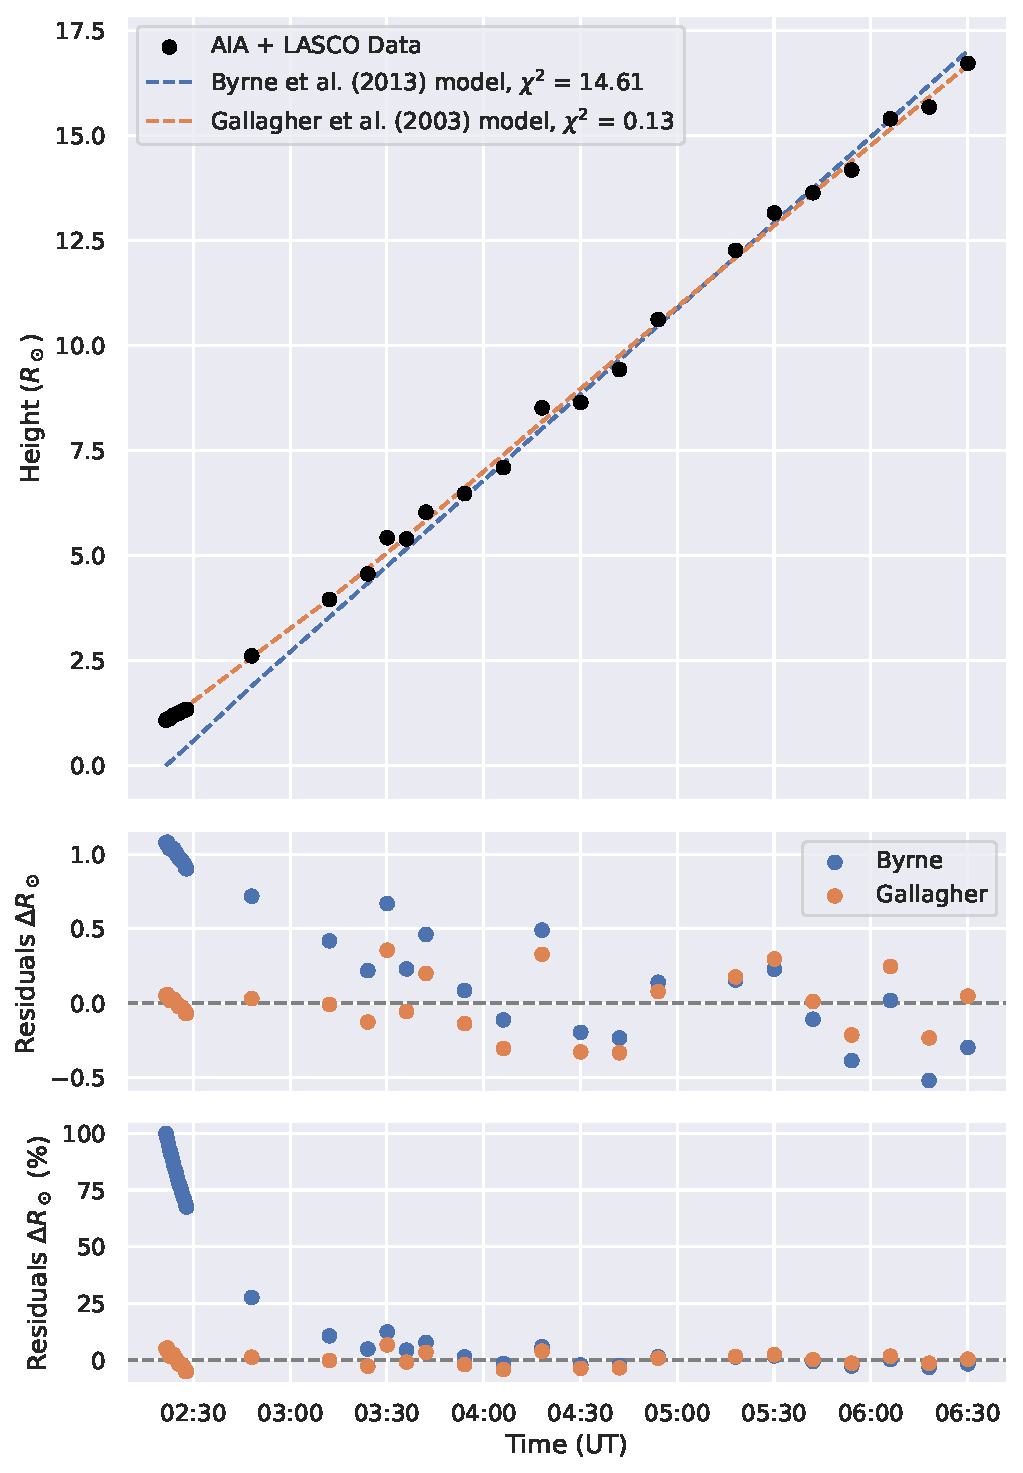
\includegraphics[width=0.7\columnwidth]{chapter2/figs/height_profile_residuals_aia_lasco_110511_01.pdf}}
	\caption{Top panel -- Height-time profile compiled from AIA and LASCO measurements for the event occurred on May 11, 2011, fitted with two CME kinematics models from the photosphere up to 17\rsun. Middle panel -- Difference between the fitting and the real observations. Bottom panel -- Relative residuals in \%.}
	\label{fig_height_profile_aialasco_110511}
\end{figure}

\begin{figure}[!htp] % updated!
	\centerline{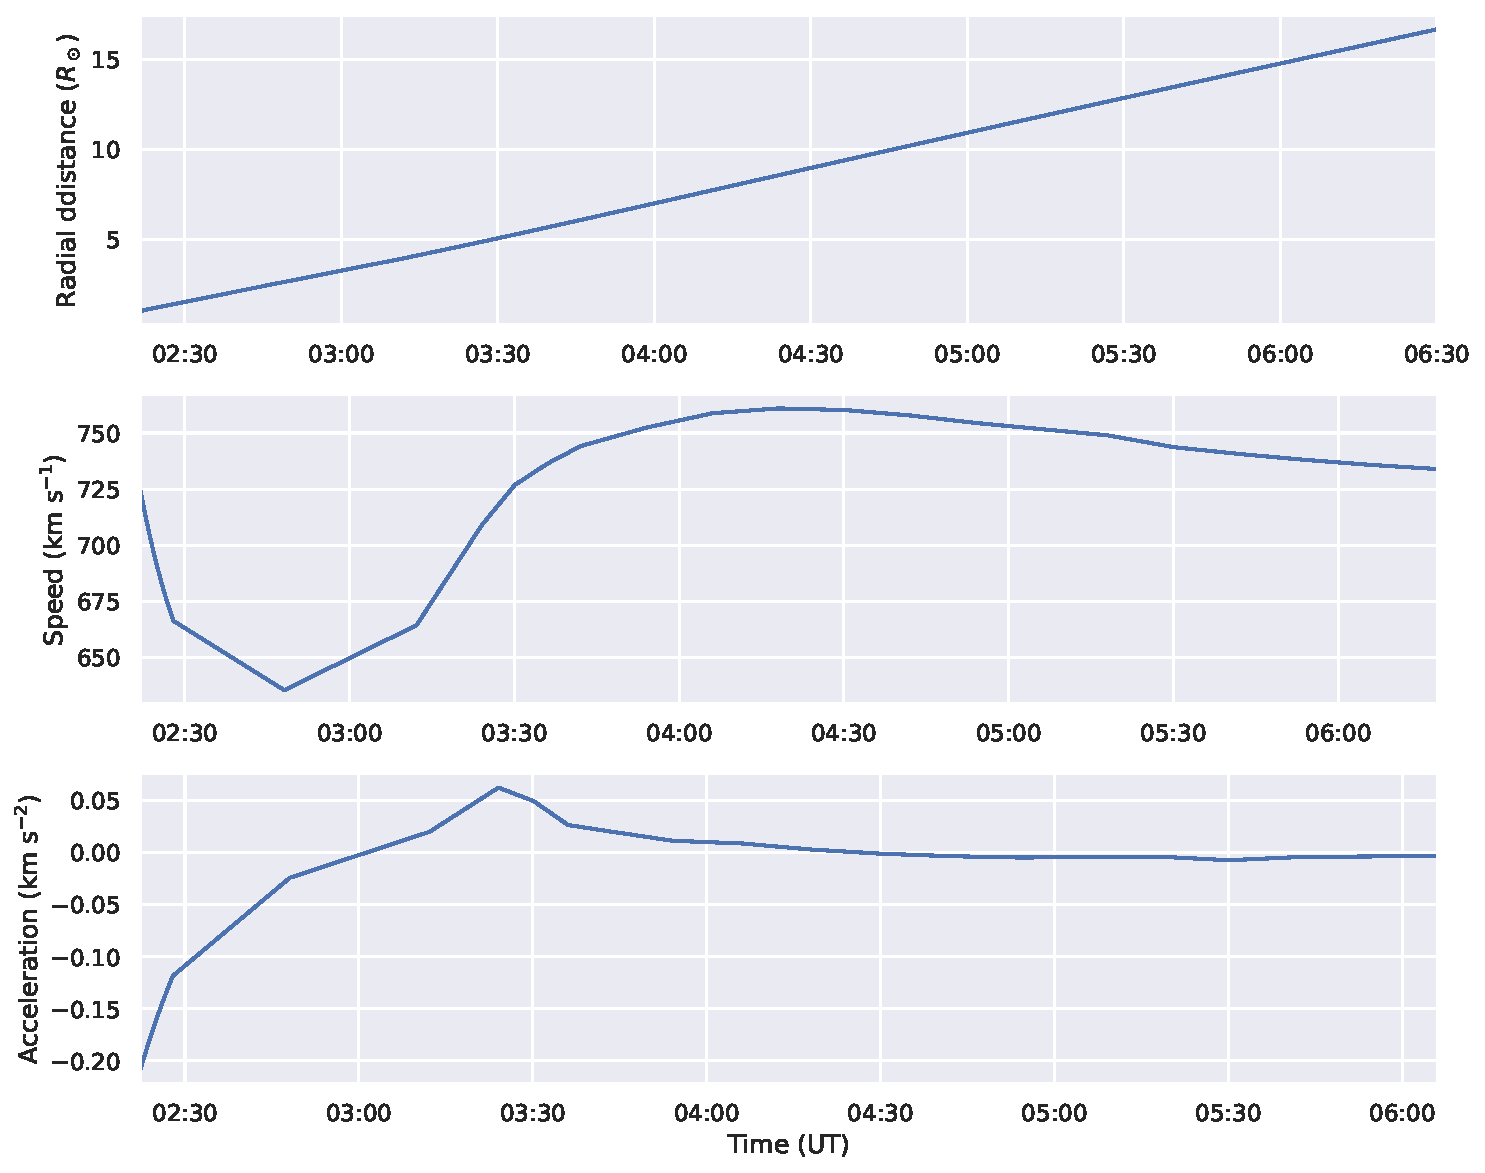
\includegraphics[width=0.8\columnwidth]{chapter2/figs/radial_kinematics_aia_lasco_110511_01.pdf}}
	\caption{Extrapolated radial kinematics for the event occurred on May 11, 2011, based on the ballistic model of \cite{gallagher_2003} up to 17\rsun.}
	\label{fig_rad_kinematics_aialasco_110511}
\end{figure}

\section{Statistical Study}
We present a comprehensive statistical analysis of the kinematic characteristics and plasma parameters of coronal wave events observed in the AIA and LASCO FOVs.

An overview of the statistical parameters related to shock characteristics, including wave speed, intensity, and thickness in the AIA FOV, is presented in Table~\ref{T_sh_param_all}. The wave speeds are expressed in \kms, wave accelerations are in km s$^{-2}$, wave intensity in arbitrary units, and wave thickness in\rsun, as the data have undergone multiple stages of processing.

Upon analyzing the data, we observed that the waves generally exhibited higher speeds, higher acceleration, lower mean intensities, and lower thickness in the radial direction compared to the lateral direction. This suggests that the waves were somewhat elongated in their early stages near the Sun, potentially due to the coronal conditions, including plasma densities and magnetic field strength and structure.

To illustrate the evolution of EUV waves' kinematics in the AIA FOV, we present Figure~\ref{fig_kinematics_spect_hist}, which provides a cumulative view of dynamic spectra for all events. The figure showcases the parameter distribution as a function of distance for shock speed, acceleration, wave intensity, and wave thickness for the radial direction (the middle column) and the lateral directions; the left and right flanks in left and right columns, respectively. The colors in the figure represent the total count in each bin at each radial position step, or each position angle step.

Consistent with our expectations, the speed and intensity panels exhibit a decline in values as a function of distance. As the waves propagate away from the Sun, the wave drivers lose momentum through interactions with the medium, leading to a decrease in speed. Additionally, plasma densities decrease with distance, resulting in a corresponding decrease in wave intensity.

\begin{table}[!htp] % updated!
	\centering
	\caption{Statistics of the EUV wave kinematics in the SDO/AIA FOV for the 26 events. LL and LR refer to the lateral left and right flanks, respectively. Rad refer to the radial front direction.}
	\label{T_sh_param_all}
	\resizebox{\textwidth}{!}{%
		\begin{tabular}{lccccccccccccc}
			\hline
			&              & \multicolumn{3}{c}{Speed (\kms)}  & \multicolumn{3}{c}{Accel. (km s$^{-2}$)} & \multicolumn{3}{c}{Intensity (DN)} & \multicolumn{3}{c}{Thickness (\rsun)} \\ \hline
			& Aspect ratio & LL      & Rad     & LR     & LL      & Rad     & LR     & LL       & Rad      & LR      & LL       & Rad      & LR      \\ \hline
			Max    & 2.00         & 1574.81 & 2053.73 & 983.58 & 28.19   & 81.01   & 13.89  & 1348.87  & 2431.95  & 1498.45 & 9.600    & 0.185    & 6.100   \\ \hline
			Min    & 0.84         & 2.11    & 40.30   & 2.30   & -35.24  & -81.01  & -9.89  & 0.53     & 0.17     & 150.30  & 0.027    & 0.018    & 0.022   \\ \hline
			Mean   & 1.87         & 316.17  & 413.60  & 264.50 & -0.15   & 0.98    & 0.13   & 438.99   & 681.46   & 442.46  & 0.715    & 0.059    & 0.231   \\ \hline
			Median & 2.00         & 284.77  & 349.32  & 216.32 & 0.03    & 0.37    & 0.11   & 337.96   & 425.23   & 389.06  & 0.102    & 0.055    & 0.076   \\ \hline
			Stdv.  & 0.33         & 261.01  & 336.11  & 191.13 & 5.53    & 11.08   & 2.05   & 292.26   & 592.78   & 227.10  & 1.721    & 0.030    & 0.776   \\ \hline
		\end{tabular}%
	}
\end{table}

\begin{figure}[!htp] % updated!
	\centerline{
		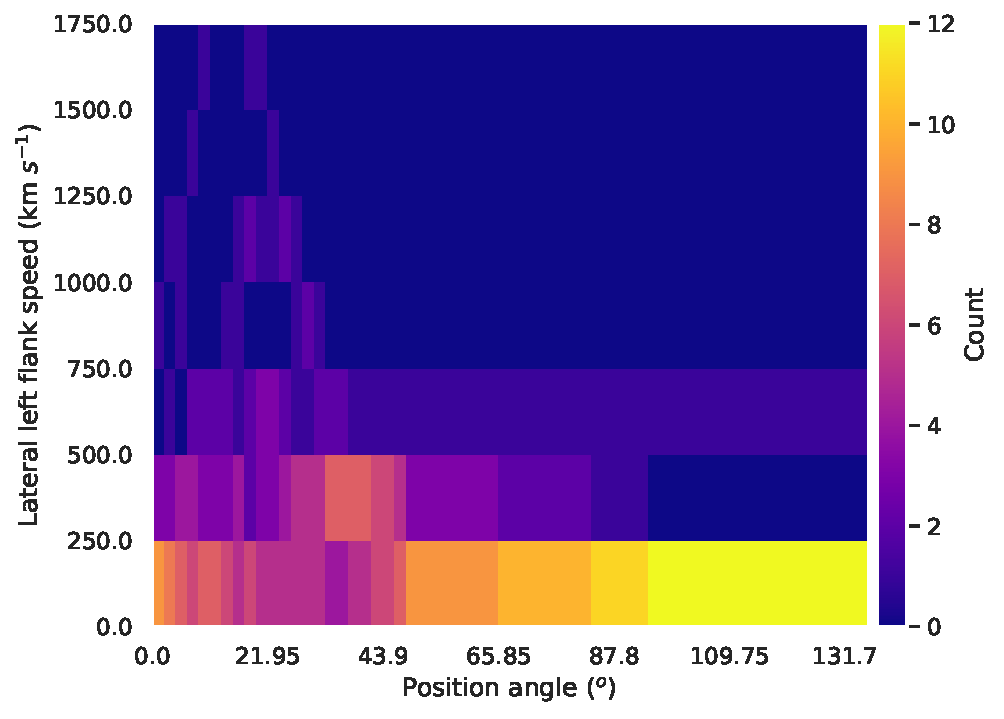
\includegraphics[width=0.32\textwidth,clip=]{chapter2/figs/latleftspd_vs_latleftpos.pdf}
		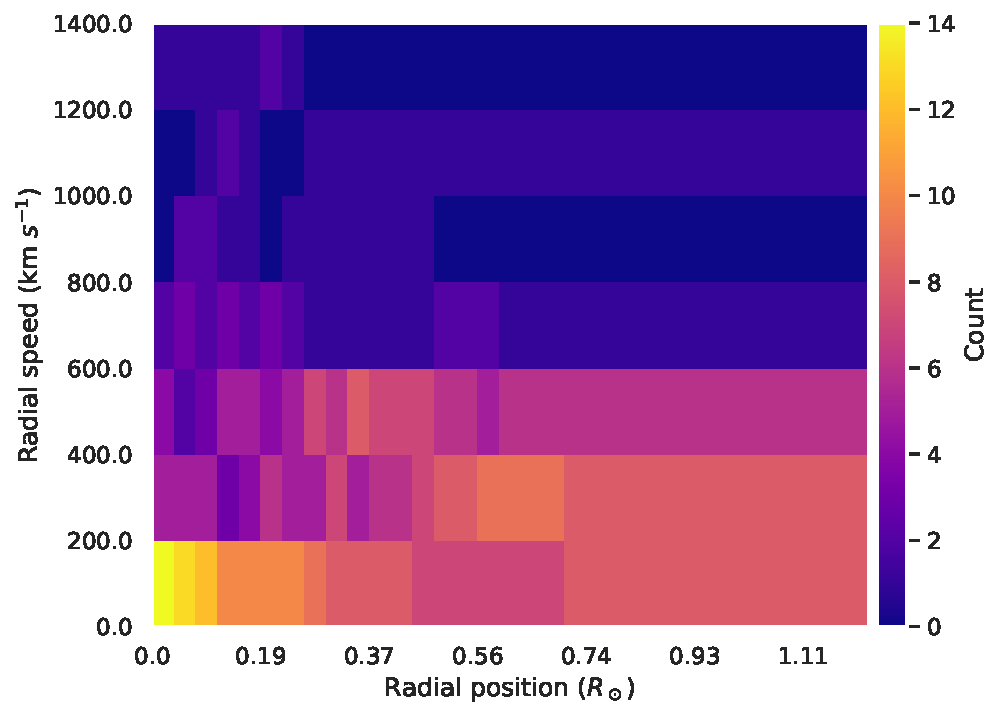
\includegraphics[width=0.32\textwidth,clip=]{chapter2/figs/radspd_vs_radpos.pdf}
		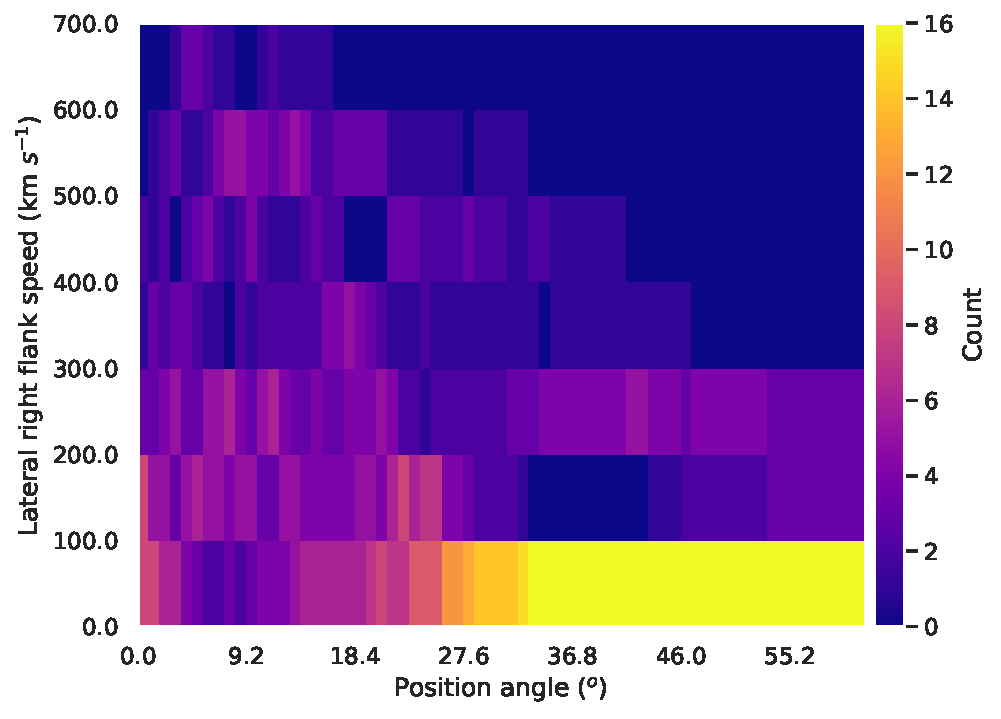
\includegraphics[width=0.32\textwidth,clip=]{chapter2/figs/latrightspd_vs_latrightpos.pdf}
	}
	\centerline{
		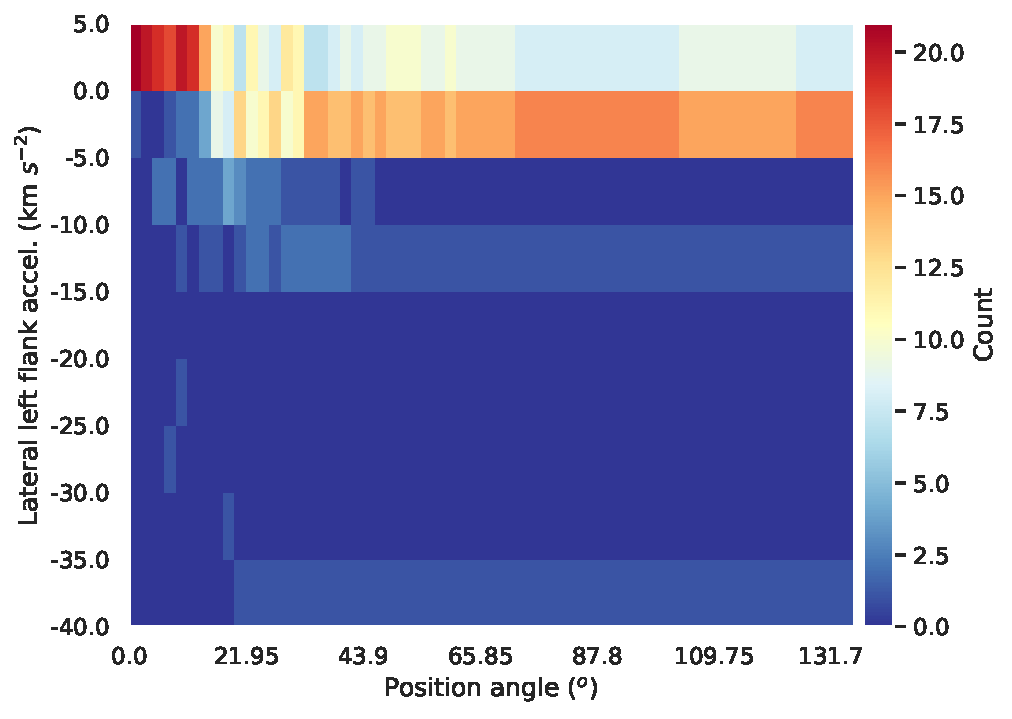
\includegraphics[width=0.32\textwidth,clip=]{chapter2/figs/latleftaccel_vs_latleftpos.pdf}
		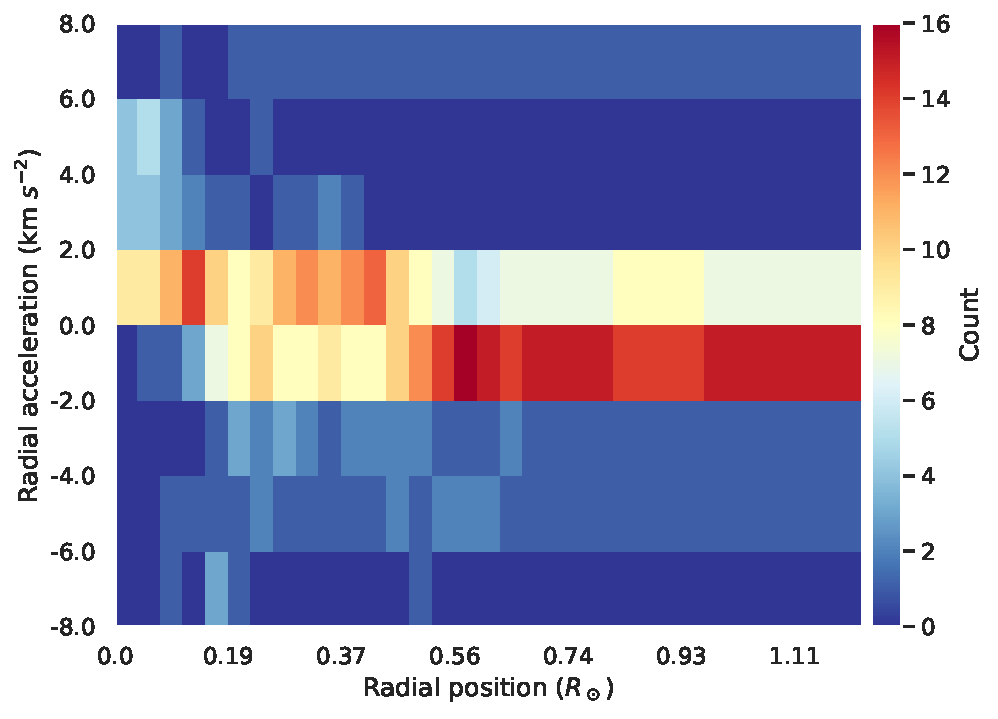
\includegraphics[width=0.32\textwidth,clip=]{chapter2/figs/radaccel_vs_radpos.pdf}
		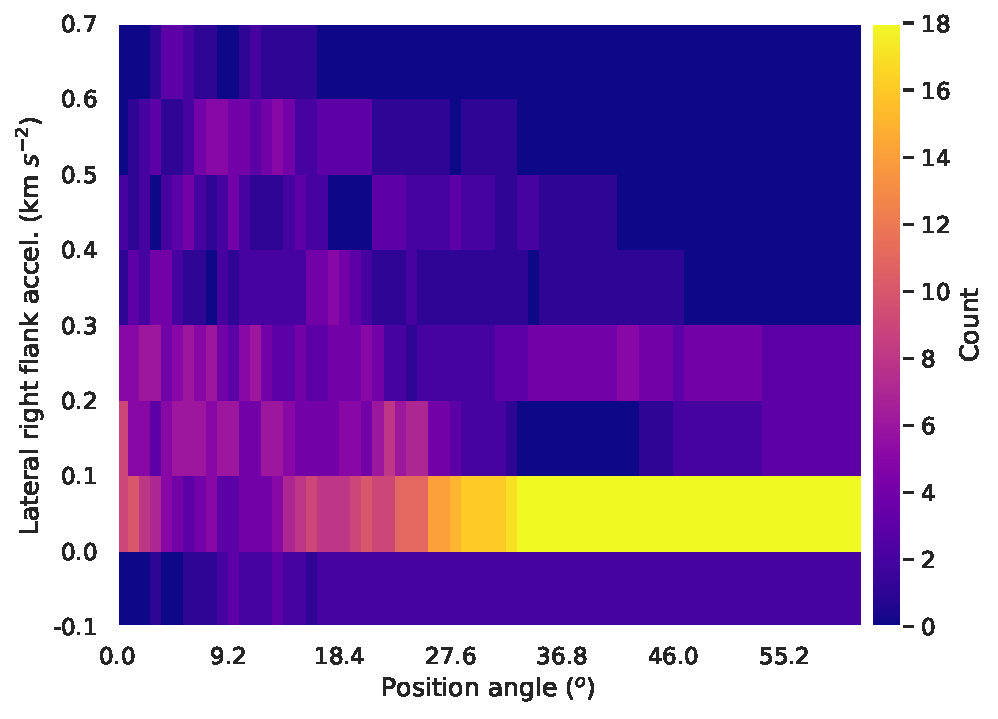
\includegraphics[width=0.32\textwidth,clip=]{chapter2/figs/latrightaccel_vs_latrightpos.pdf}
	}
	\centerline{
		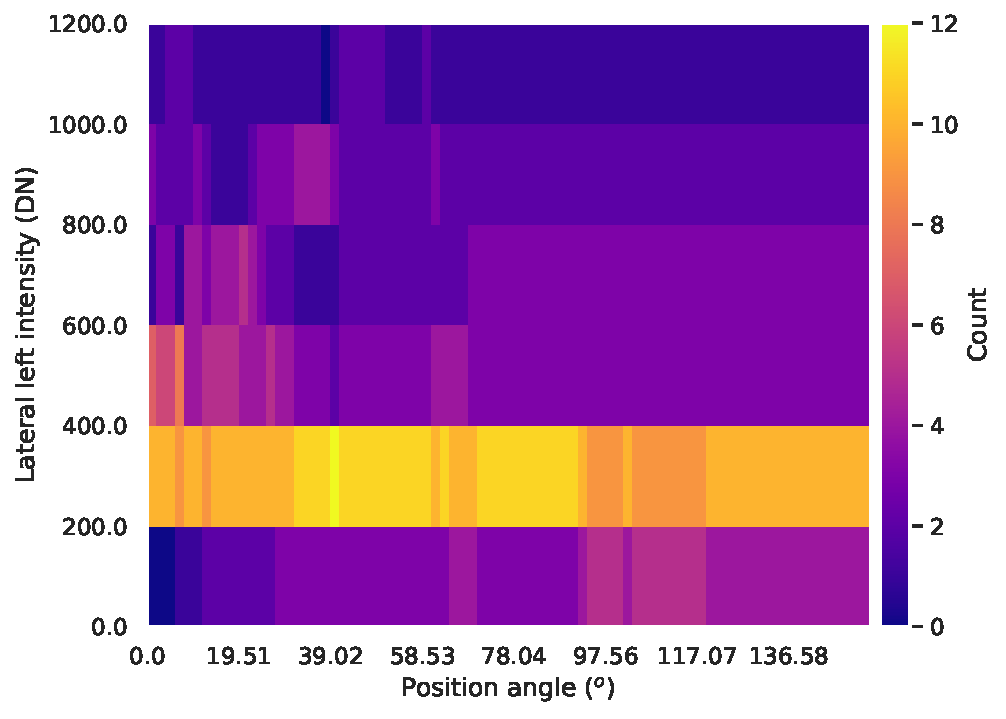
\includegraphics[width=0.32\textwidth,clip=]{chapter2/figs/latleftint_vs_latleftpos.pdf}
		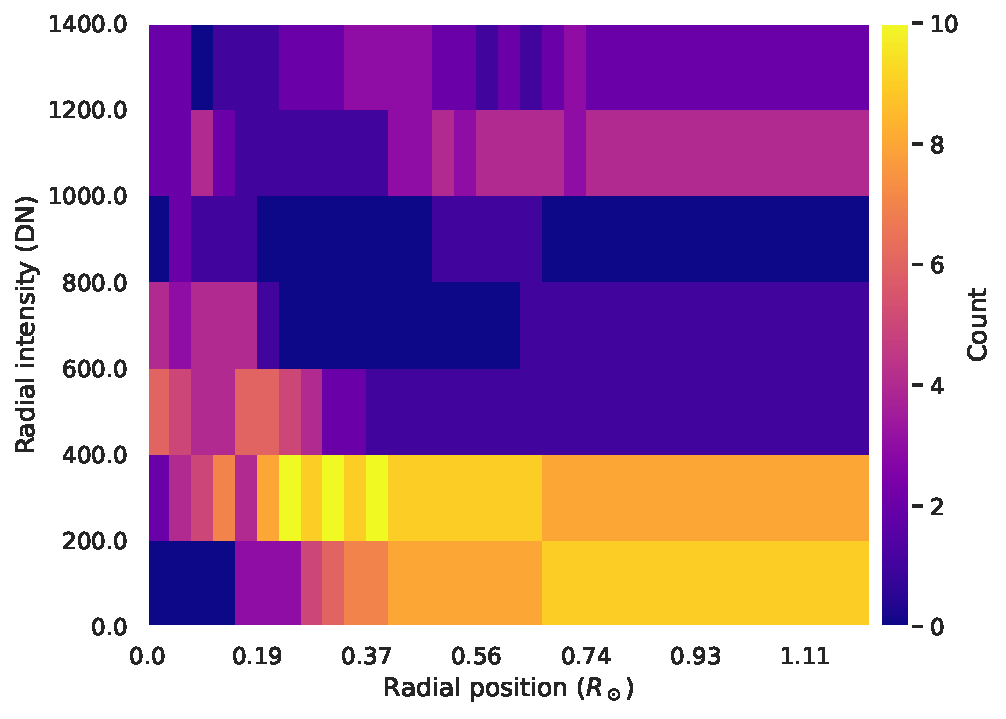
\includegraphics[width=0.32\textwidth,clip=]{chapter2/figs/radint_vs_radpos.pdf}
		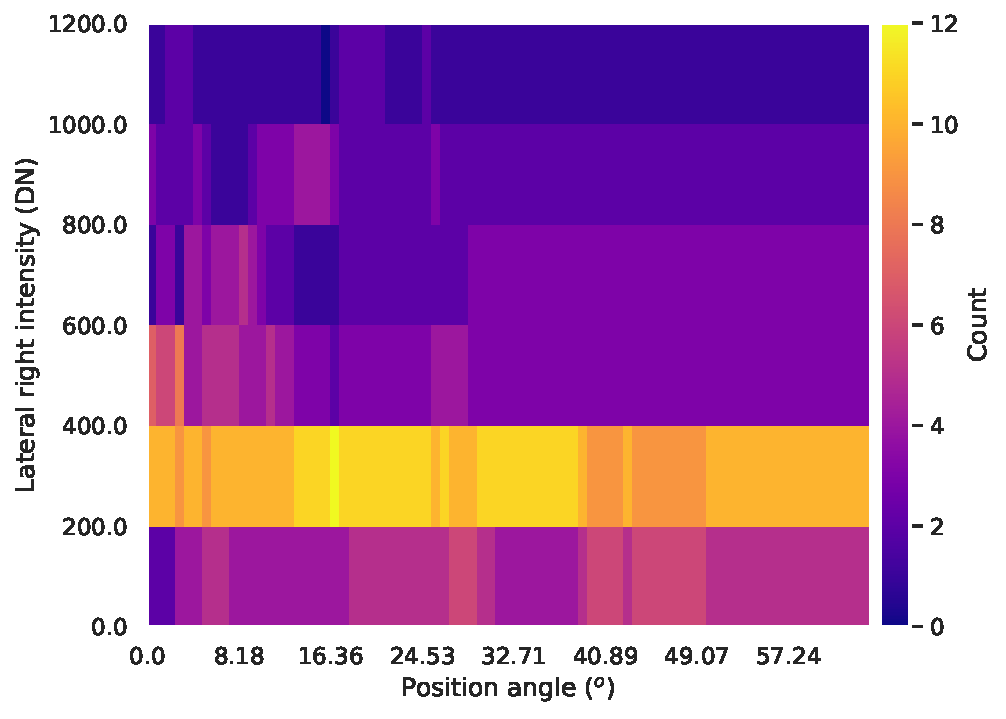
\includegraphics[width=0.32\textwidth,clip=]{chapter2/figs/latrightint_vs_latrightpos.pdf}
	}
	\centerline{
		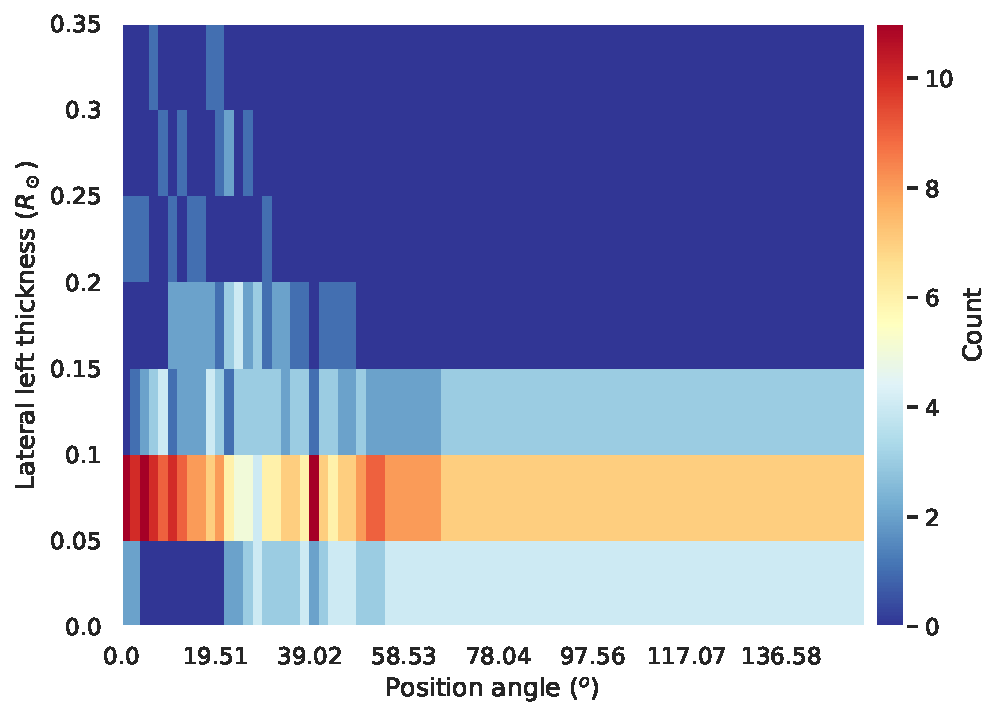
\includegraphics[width=0.32\textwidth,clip=]{chapter2/figs/latleftthick_vs_latleftpos.pdf}
		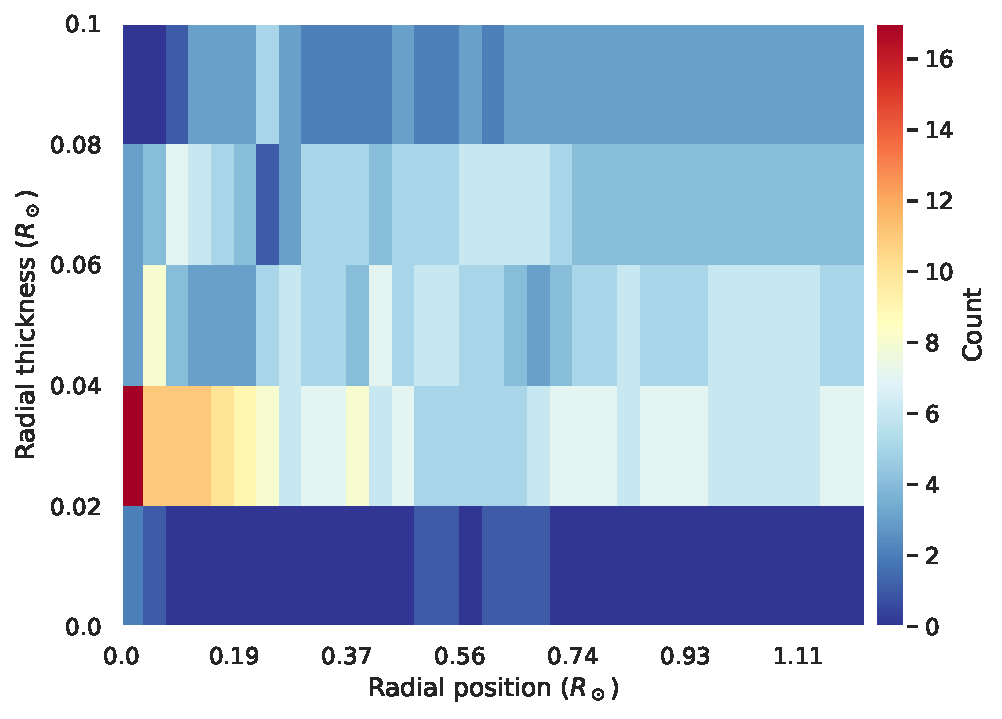
\includegraphics[width=0.32\textwidth,clip=]{chapter2/figs/radthick_vs_radpos.pdf}
		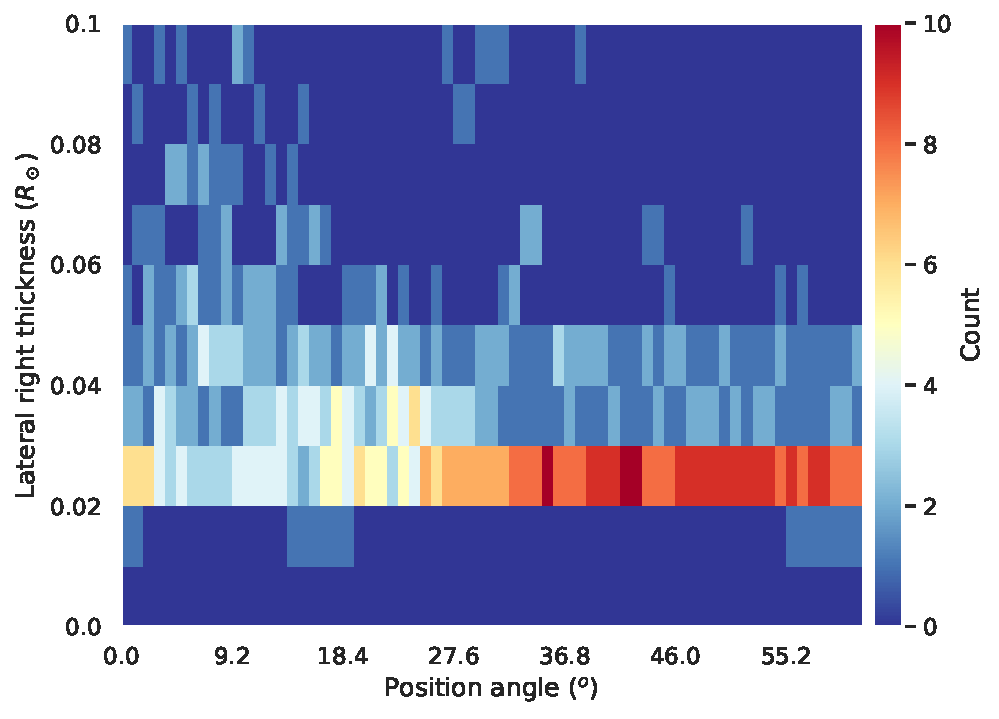
\includegraphics[width=0.32\textwidth,clip=]{chapter2/figs/latrightthick_vs_latrightpos.pdf}
	}
	\caption{Dynamic spectra of the EUV waves kinematics in the AIA FOV. The panels from the top to the bottom are the wave speeds, acceleration, mean intensity, and thickness. The left column is for the lateral left flank, the central column is for the radial direction, and the right column is for the lateral right flank.}
	\label{fig_kinematics_spect_hist}
\end{figure}

To investigate the bulk behavior of the modeled plasma above and at the shock surface, we sampled over 1000 field lines from the 26 events. The resulting histograms, shown in Figures~\ref{fig_hist_plasma_param_corr}, reveal correlations between various pairs of parameters. 
We investigated the correlations between five parameters -- the shock-field angle (\textbf{THBN}), the coronal magnetic field (\textbf{BMAG}), the plasma density (\textbf{DENSITY}), the Alfven speed (\textbf{VA}), the shock speed (\textbf{VSHOCK}), and the shock density jump (\textbf{SHOCKJUMP}).

The histograms show that there are weak to moderate correlations between some of the parameters.
For example, there is a moderate positive correlation between \textit{BMAG} and \textit{DENSITY}, and a moderate positive correlation between \textit{BMAG} and \textit{VA}. These correlations suggest that there may be some underlying physical processes that connect these two parameters.
The positive correlation between \textit{BMAG} and \textit{DENSITY} could be due to the fact that stronger magnetic fields can compress the plasma, leading to higher densities.
The negative correlation between \textit{BMAG} and \textit{VA} could be due to the fact that stronger magnetic fields tend to speed up the Alfven waves.

In addition to the anticipated correlations between the Alfven speed with magnetic field and density, we discovered a highly skewed correlation between magnetic field values and the modeled shock density jump, as well as between magnetic field magnitude and density.
The negative correlation between \textit{BMAG} and \textit{SHOCKJUMP} indicates that stronger coronal magnetic fields are associated with smaller density jumps across the shock surface. In other words, weak magnetic field correlates well with stronger shocks.
This could be due to several possible mechanisms. For instance, stronger magnetic fields exert higher pressure, potentially resisting the compression of plasma by the shock wave, leading to a smaller density increase across the shock front.
In addition, as mentioned earlier, stronger magnetic fields might lead to faster Alfven waves, allowing the plasma ahead of the shock to react and reduce the density jump.
These correlations will be further explored to establish a more definitive connection and to parameterize the shock density jump.

\begin{figure}[!htp] % updated!
	\centerline{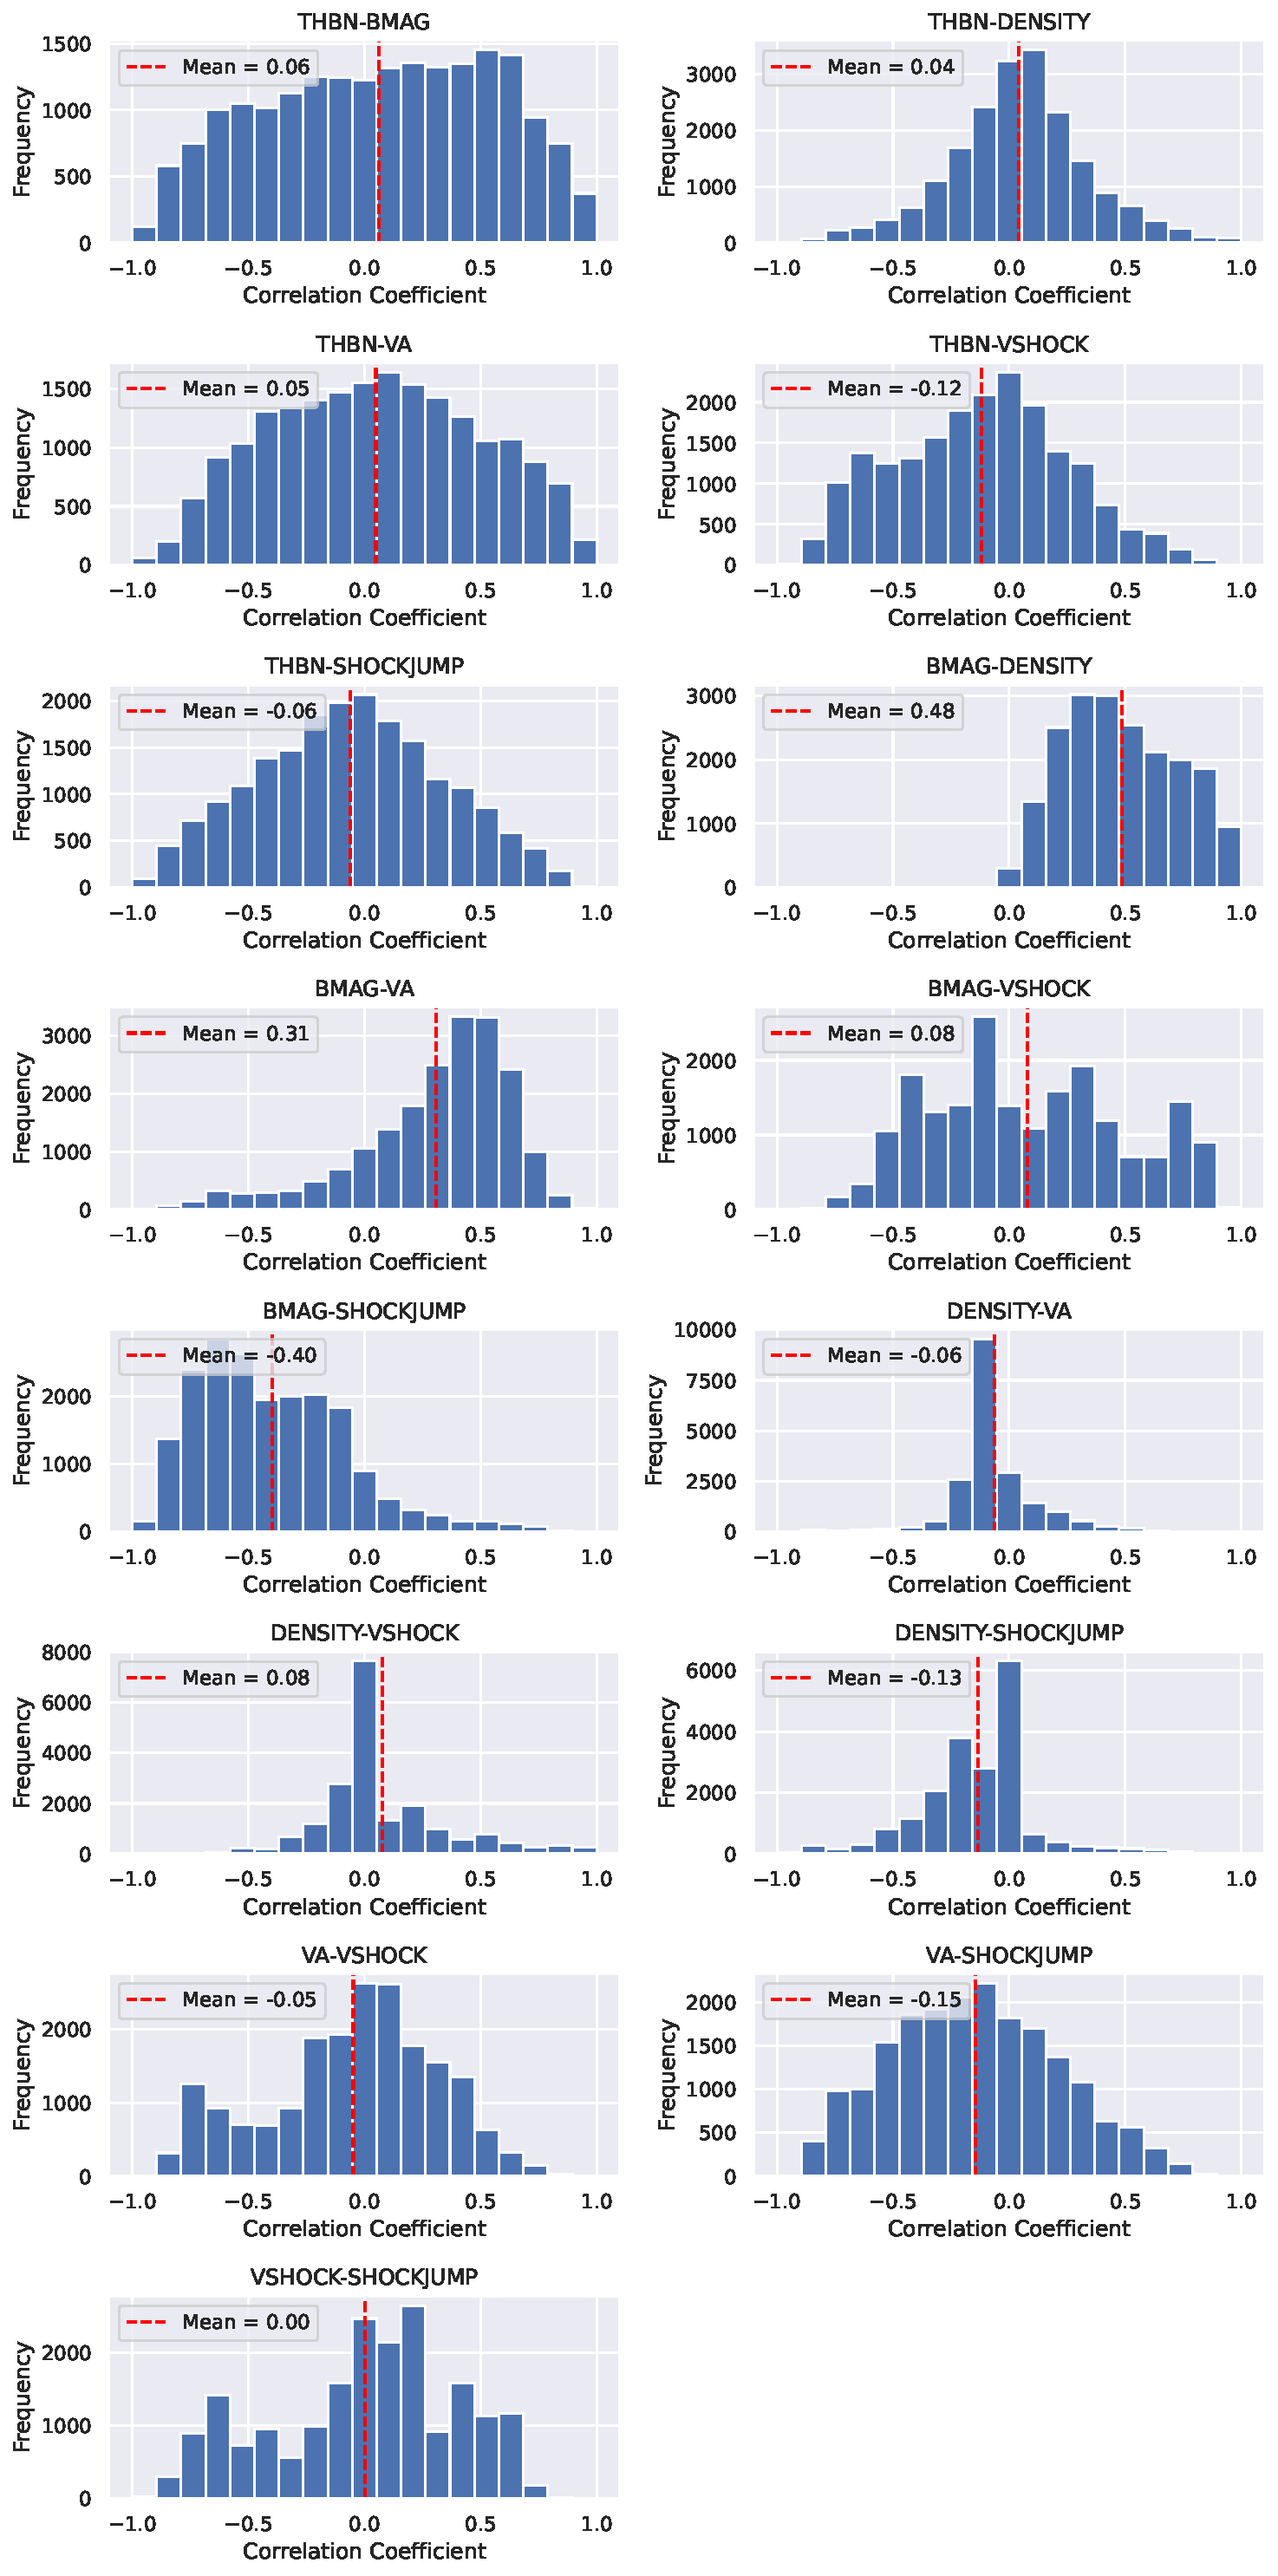
\includegraphics[width=0.7\columnwidth]{chapter2/figs/wp3_d2_Fig16.pdf}}
	\caption{Histograms of along-field-lines model plasma parameters in the solar corona for all the 26 events. The vertical dashed red lines are the mean values.}
	\label{fig_hist_plasma_param_corr}
\end{figure}

We also aim to investigate the event-averaged modeled plasma parameters and establish the observed connections between these parameters throughout entire events. To achieve this, we computed the mean, maximum, and summed values of the parameters for each event. The analysis revealed a set of parameter pairs that exhibit promising relationships suitable for parameterization. Among these pairs, we selected six representative cases for further examination.

The scatter plots presented in Figure~\ref{fig_scatterplot_plasma_param} depict the chosen modeled parameter pairs. From left to right, top to the bottom, we plotted the logarithm of the summed values of the shock-field angle $\theta_{BN}$ versus the logarithm of the summed values of the absolute coronal magnetic field (A), the logarithm of the summed values of $\theta_{BN}$ versus the mean values of the shock speed (B), the logarithm of the summed values of $\theta_{BN}$ versus the logarithm of the summed values of the shock speed (C), the logarithm of the summed values of $\theta_{BN}$ versus the logarithm of the summed values of the shock density jump (D), the mean values of the absolute magnetic field versus the mean values of the shock speed (E), the logarithm of the summed values of the Alfven speed versus the mean values of the shock speed (F), the mean values of the shock speed versus the mean values of the density jump (G), and finally the logarithm of the summed values of the Alfven speed versus the mean values of the density jump (H).

To determine the best-fitting equations, we tested several models and found that power fits yield the most accurate results in this particular case. The graphs illustrating the fit parameters and the $\chi^2$ are provided for reference.

%The scatter plot analysis reveals strong correlations among all parameter pairs, indicating the presence of hidden connections between these parameters. It is important to note that some outliers exist, but they do not undermine the overall correlation patterns.
%In the subsequent phase of our project, we will focus on developing and testing parameterizations for these identified connections. Our ultimate objective is to establish a set of synoptic MHD parameters that correspond one-to-one with the parameters we measure, such as shock density jump and shock speed. By accomplishing this, we will enhance the representation of shock parameters in the \textit{S3M} synoptic model, even in the absence of actual compressive waves.

The analysis of eight figures examining shock dynamics in EUV wave events revealed significant findings. In Figure (A), a weak positive correlation between coronal magnetic field strength and shock-field angle was observed, suggesting a nuanced relationship influenced by factors beyond magnetic fields. Figure (B) showcased a weak negative correlation between shock-field angles and mean shock speeds, hinting at a connection between complex shock geometries and slower wave speeds. In Figure (C), there appears to be a weak negative correlation between the logarithm of the shock-field angle and the logarithm of the sum of shock speeds, which is indicated by the faintly downward-sloping trendline. This hints at a slight tendency for larger shock-field angles to be associated with slower shock speeds. Figure (D) displayed a moderate positive correlation between shock density jump and shock-field angles, suggesting potential interactions between shock wave geometry and density variations.

Meanwhile, Figures (E), (F), (G), and (H) delved into relationships between solar coronal magnetic field strength, shock speeds, Alfven speeds, and shock density jumps, revealing negative, lack of clear, and lack of consistent correlations, respectively. These findings emphasize the intricate nature of solar coronal shock dynamics, with multiple influencing factors contributing to observed correlations and scattering in the data. The comprehensive analyses underscore the need for more events and a nuanced understanding of various factors when interpreting the complexities of shock phenomena in the solar corona.

It is important to note that some outliers exist, but they do not undermine the overall correlation patterns. In future work, we will focus on developing and testing parameterizations for these identified connections in order to establish a set of synoptic MHD parameters that correspond one-to-one with the parameters we measure, such as shock density jump and shock speed. By accomplishing this, we will enhance the representation of shock parameters even in the absence of actual compressive waves.

\begin{figure}[!htp] % updated!
	\centerline{
		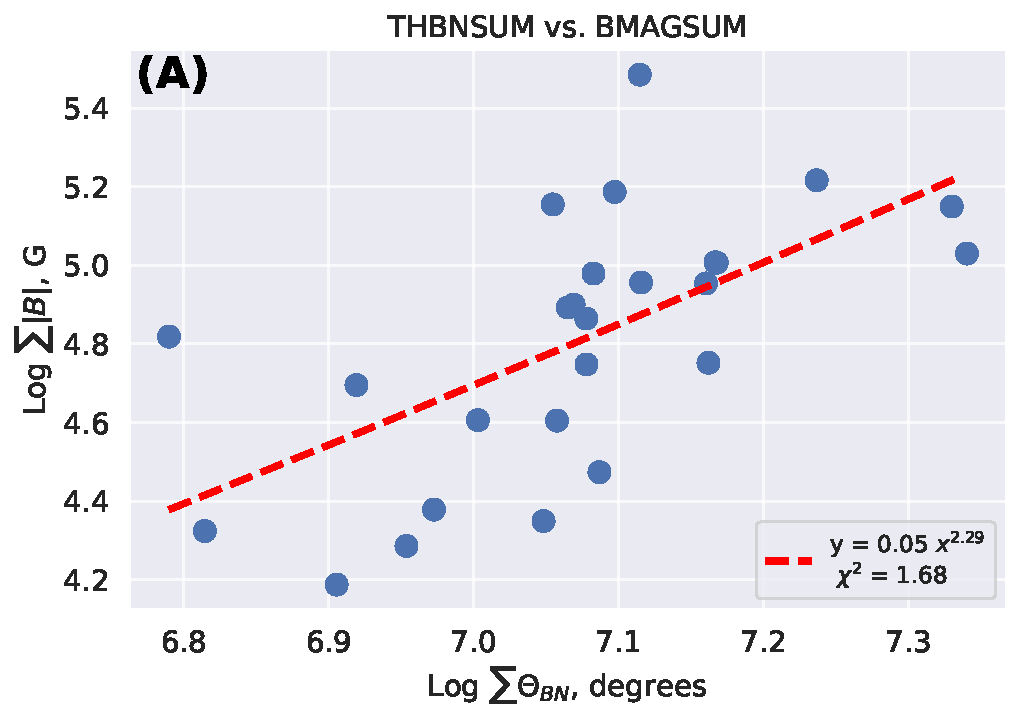
\includegraphics[width=0.45\textwidth]{chapter2/figs/THBNSUM_BMAGSUM.pdf}
		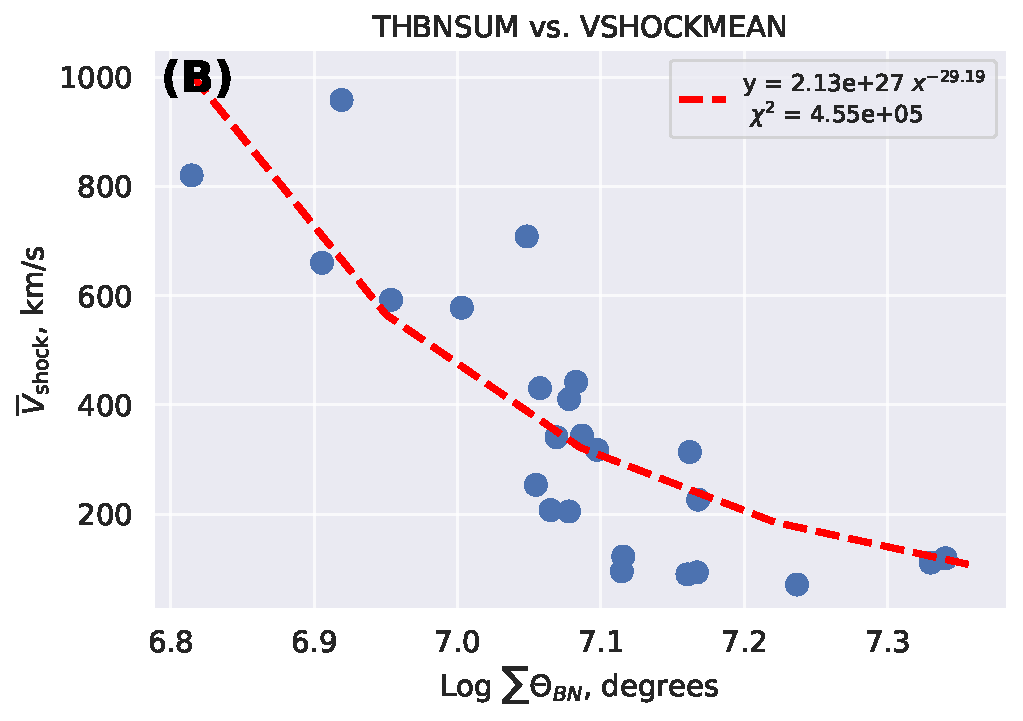
\includegraphics[width=0.45\textwidth]{chapter2/figs/THBNSUM_VSHOCKMEAN.pdf}
	}
	\centerline{
		\includegraphics[width=0.45\textwidth]{chapter2/figs/THBNSUM_VSHOCKSUM.pdf}
		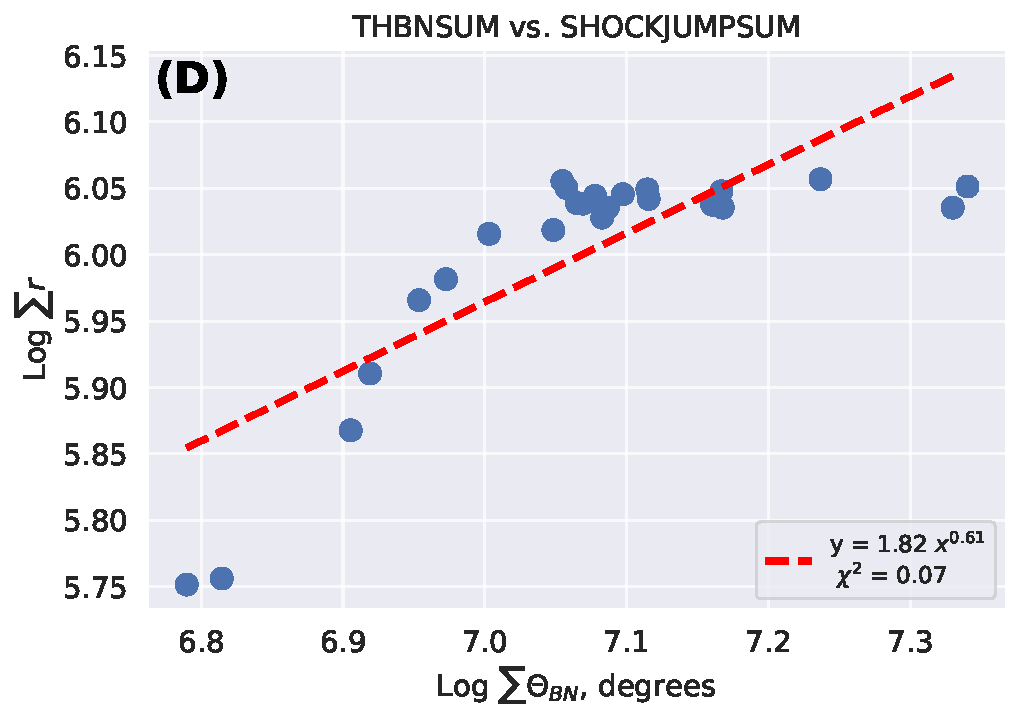
\includegraphics[width=0.45\textwidth]{chapter2/figs/THBNSUM_SHOCKJUMPSUM.pdf}
	}
	\centerline{
		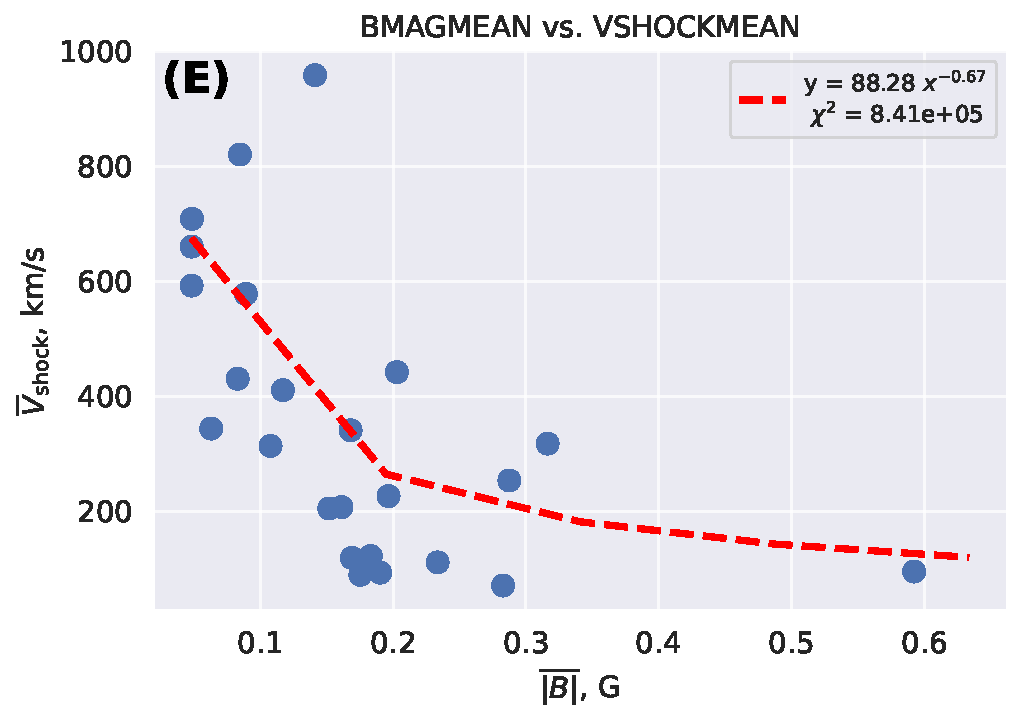
\includegraphics[width=0.45\textwidth]{chapter2/figs/BMAGMEAN_VSHOCKMEAN.pdf}
		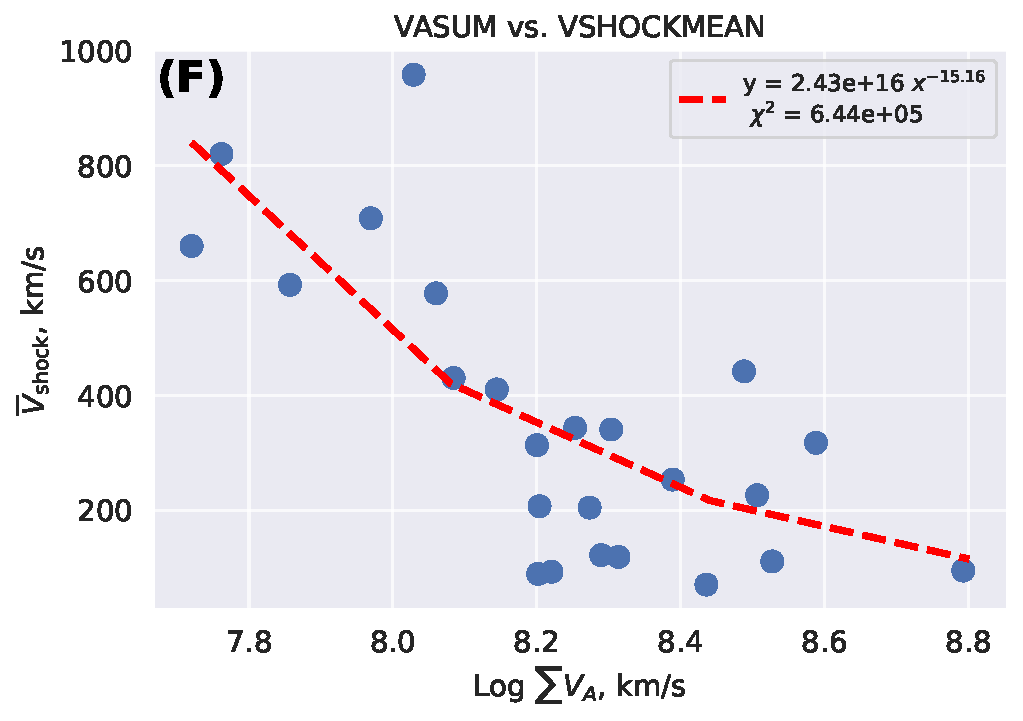
\includegraphics[width=0.45\textwidth]{chapter2/figs/VASUM_VSHOCKMEAN.pdf}
	}
	\centerline{
		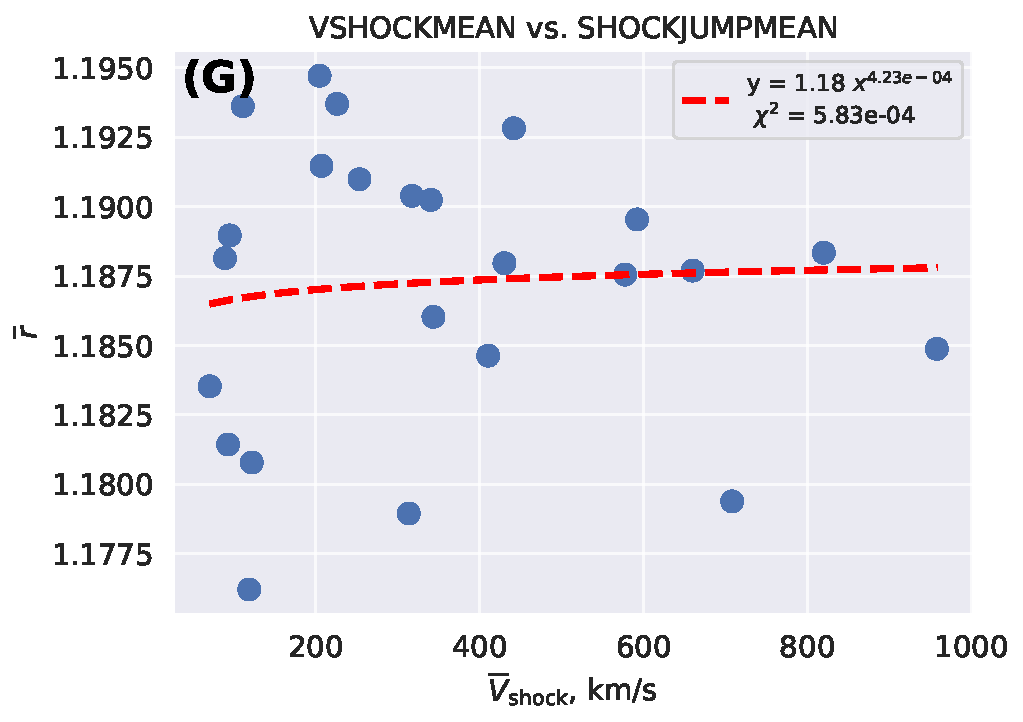
\includegraphics[width=0.45\textwidth]{chapter2/figs/VSHOCKMEAN_SHOCKJUMPMEAN.pdf}
		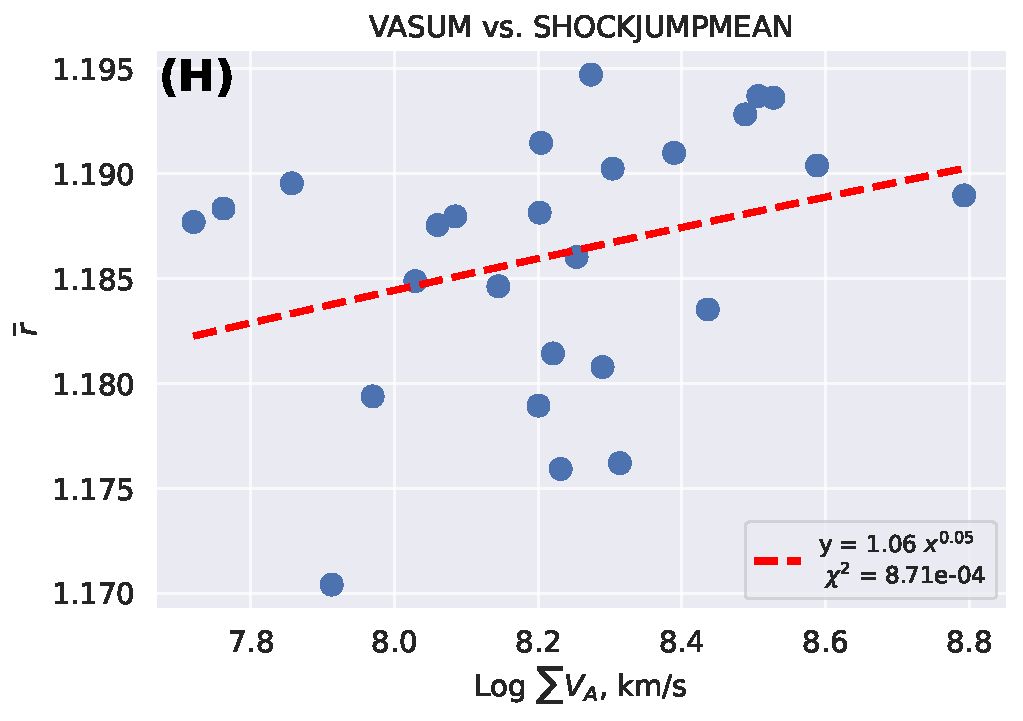
\includegraphics[width=0.45\textwidth]{chapter2/figs/VASUM_SHOCKJUMPMEAN.pdf}
	}
	\caption{Scatter plots of 8 coronal plasma-parameter pairs that exhibit parameterizable relationships. The \textit{VSHOCKMEAN} is filtered to take only events with speeds $<$4000 \kms.}
	\label{fig_scatterplot_plasma_param}
\end{figure}

%%% From Kozarev paper ...
%To characterize the kinematics of CBFs, we implement the methodology of the Coronal Analysis of Shocks and Waves (CASHeW) framework, as proposed by \citet{kozarev_2017}, within the SPREAdFAST framework. This methodology has been further refined and updated. Our approach aligns with the techniques presented by \citet{long_2021} and \citet{downs_2021}, where we track the leading edge of the CBF front across consecutive AIA images. Additionally, we compute the kinematics of the peak and back edge of the CBFs over time, enabling the estimation of their time-dependent mean intensity and thickness.

%Figure~\ref{fig_cbf_110511} exemplifies the application of this methodology to the CBF event on May 11, 2011. Panel A displays a mid-event AIA 193-channel base difference image, clearly illustrating the CBF. Radial and lateral lines of measurement are overlaid on the image. The kinematics of the CBF are identified using the J-maps, as explained in the previous section. The radial direction measurements (Panel B) are taken along the line passing through the solar center and the CBF nose (predominant direction of motion). Lateral wave front signatures are measured in two directions away from the radial direction (Panels C and D), parallel to the solar limb. The lateral measurements in both directions are averaged to form a single lateral kinematics time series for each event. The resulting CBF width and mean intensity in both directions are also recorded.

%\begin{figure}[htp]
%	\centering
%	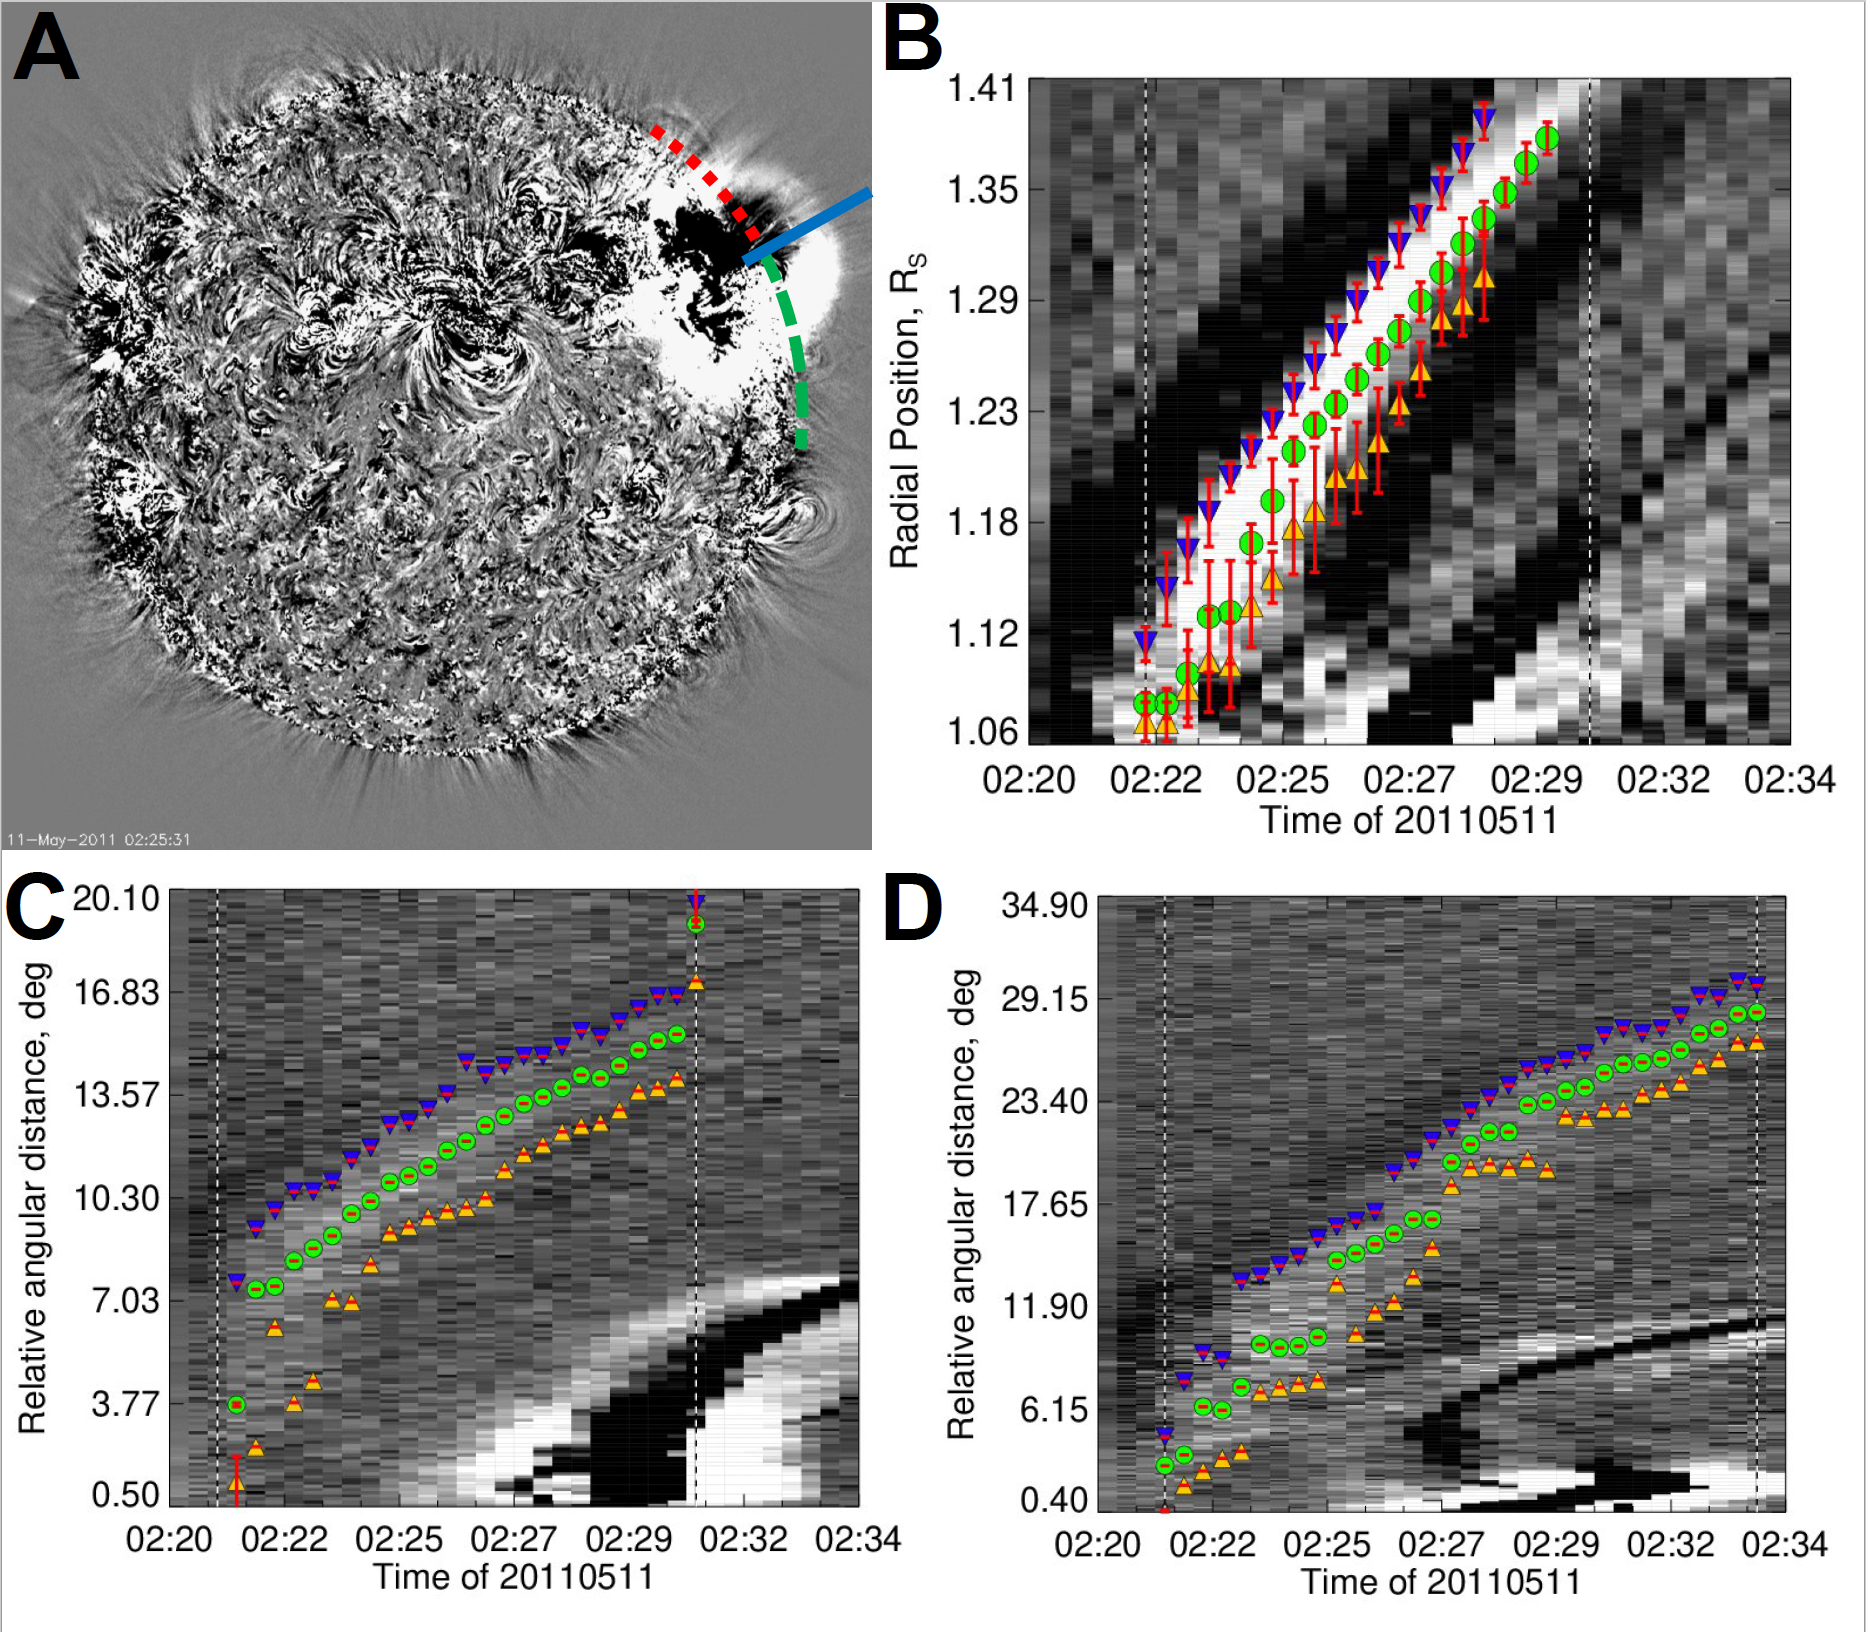
\includegraphics[width=0.9\hsize]{chapter2/figs/fig_110511_kinematics.jpg}
%	\caption{Kinematic analysis of the CBF associated with the May 11, 2011 solar eruption. (A) SDO/AIA 193\AA base difference image displaying the erupting CBF. The blue solid line shows radial measurement direction; red dotted and green dashed arcs indicate lateral directions. (B) Radially measured CBF kinematics, including time-distance J-map and average front, peak, and back positions, quantifying expansion rate. (C) Northward and (D) southward lateral kinematic measurements and J-maps. Credit goes to \citet{kozarev_2022}.}
%	\label{fig_cbf_110511}
%\end{figure}

%To obtain the kinematics in the AIA FOV, a Savitzky-Golay fit is applied, following the method proposed by \citet{kozarev_2019}. The smoothed positions are then extrapolated to 10\rsun using the analytical model of \citet{byrne_2013}. Based on the measured front positions over time, a three-dimensional, time-dependent geometric spheroid model named Synthetic Shock Model (S2M) is developed for all compressive fronts. This model, consisting of over 1000 points, is utilized to estimate the dynamic shock upstream coronal parameters. Figure~\ref{fig_segments} illustrates 9 time steps of the S2M for an eruption near the northwest limb of the Sun.

%The spheroid, centered on the eruption source, maintains its aspect ratio throughout the event. Once the S2M wraps around the Sun, points behind the plane passing through the eruption source point, and perpendicular to the radial direction at that point, are removed from consideration. The S2M is divided into a cap and two side zones, denoted by blue, green, and red points in Figure~\ref{fig_segments}. This division allows for the investigation of variations in the plasma environment as the CBF traverses in the radial and lateral directions.

%The \textit{nose} of the shock model is defined as the collection of all model points on the spheroidal cap subtending a half-angle of $\pi$/7 from the semi-major axis of the spheroid at each time step. The remaining points on the shock surface are divided into two flanks or zones, with the dividing plane parallel to the Sun-Earth line. Plasma parameters at points on these three surfaces can be examined separately, providing insights into the differences in the plasma environment through which the CBF passes, as demonstrated in Figure~\ref{fig_segments}.

Figure~\ref{fig_mean_densjump_all} depicts the temporal evolution of the mean shock density jump ($r$) for the 26 events within the studied sample. Each data point represents the average value across all shock-crossing points for the respective timestep and event. All modeled events were constrained to 50 timesteps, each lasting 24 seconds. Consequently, the graph illustrates the mean aspect ratio for all events at each timestep. The profile exhibits an initial relatively low value of 1.2, gradually rising to nearly 1.4 before gradually returning to 1.2. The semi-transparent blue shading denotes the standard deviation error at each timestep.

\begin{figure}[!htp] % updated!
	\centerline{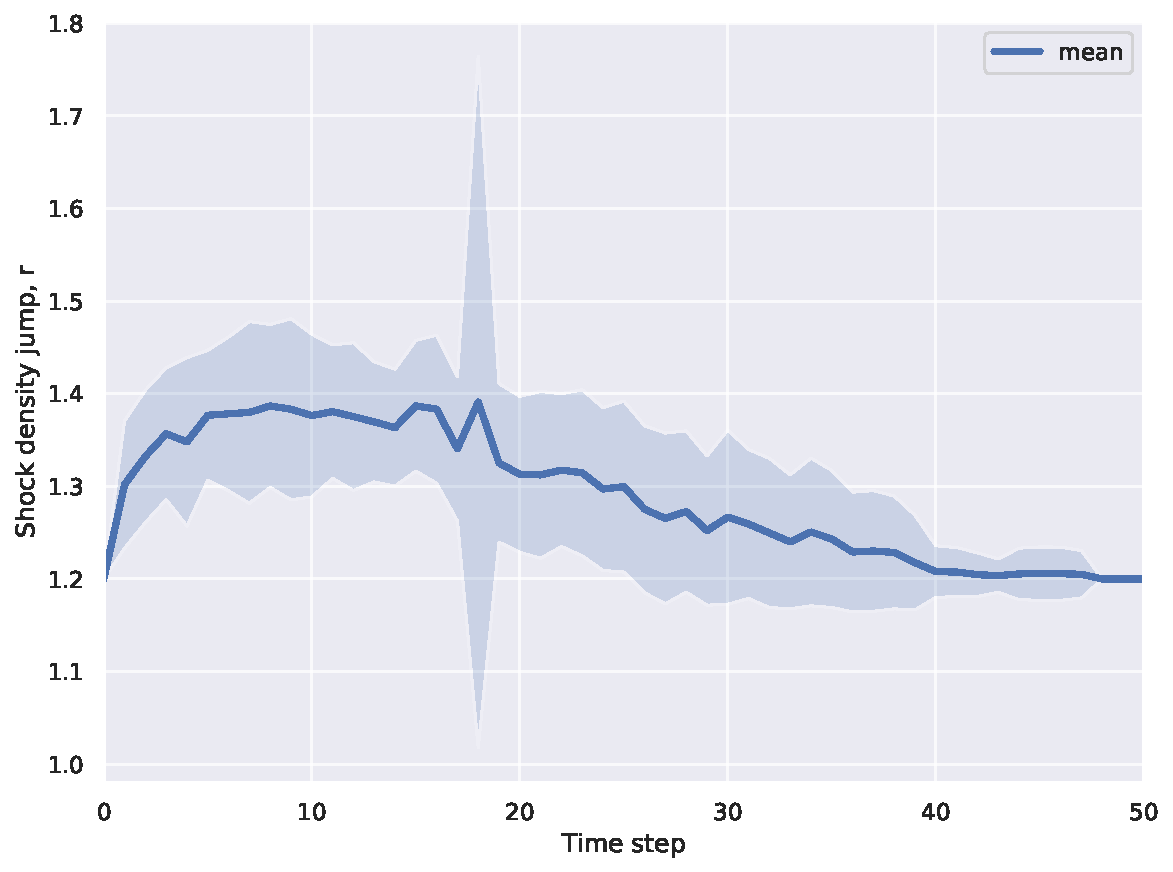
\includegraphics[width=0.8\columnwidth]{chapter2/figs/mean_densityjump_stat.pdf}}
	\caption{Time profile of the mean shock density jump for the 26 in-sample historical events studied with SPREAdFAST.}
	\label{fig_mean_densjump_all}
\end{figure}

Finally, in Figure~\ref{fig_mean_aspectratio_all}, I present the computed mean value of time-dependent aspect ratios for all events within our study. The analysis encompasses events confined to 50 timesteps, each lasting 24 seconds. Consequently, the graph illustrates the average aspect ratio across all events at each timestep, revealing a noticeable decrease in aspect ratio. This profile serves as a foundational reference for subsequent modeling phases in SPREAdFAST.

\begin{figure}[!htp] % updated!
	\centerline{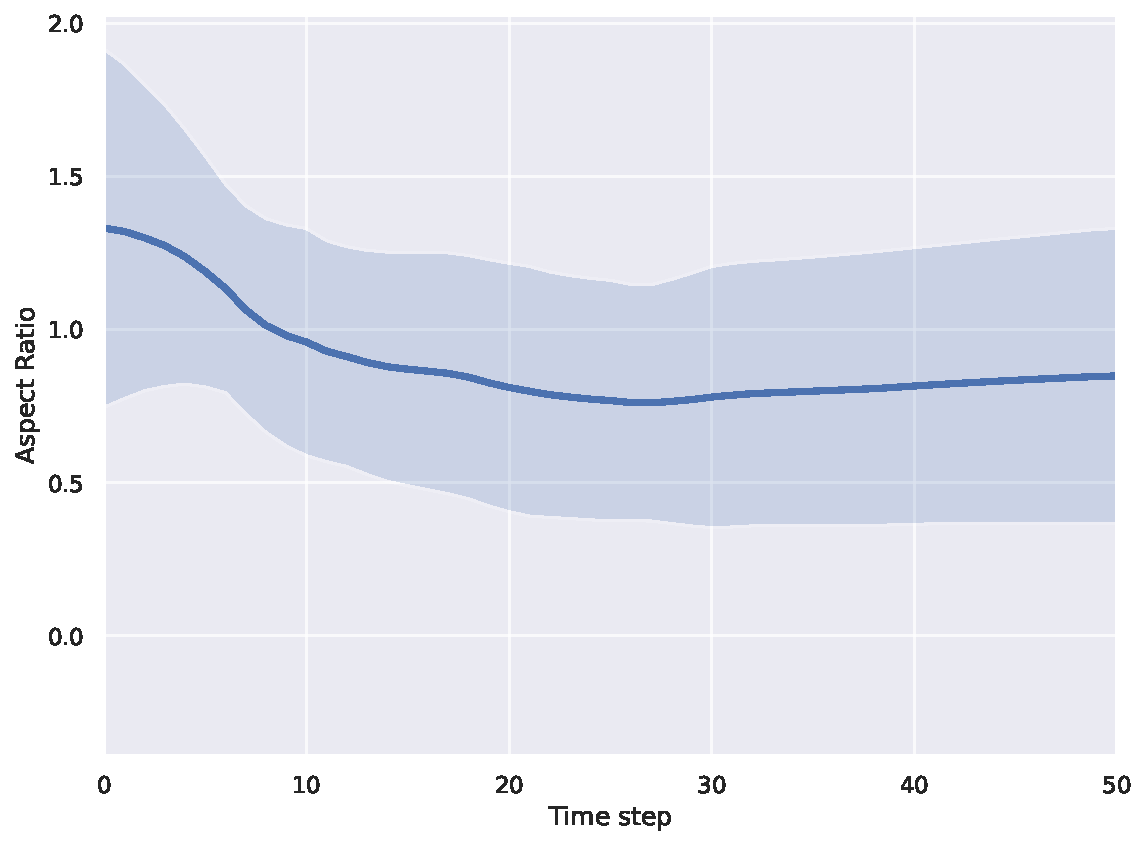
\includegraphics[width=0.8\columnwidth]{chapter2/figs/mean_aspectratio_stat.pdf}}
	\caption{Time profile of the mean aspect ratio of the 26 historical events studied with SPREAdFAST.}
	\label{fig_mean_aspectratio_all}
\end{figure}

%%%%%%%%%%%%%%%%%%%%%%%%%%%%%%%%%%%%%%%%%%%%%%%%%%%%%%%%%%%%%%%%%%%%%%%%%%%%%%%%%%%%%%%%

\section{Wavetrack: A Flexible Framework for Automated Recognition and Tracking of Wave-Like Events in Solar Imagery}
\subsection{Overview}
Solar eruptive events encompass a myriad of intricate phenomena, including flares, filament eruptions, coronal mass ejections (CMEs), and CME-driven shock waves. The principal drivers of solar energetic particles (SEPs) are acknowledged to be CME-driven shocks within the corona and interplanetary space. This acceleration primarily occurs through the diffusive shock acceleration (DSA) and shock drift acceleration (SDA) processes \citep{reames_2021}. Efforts have been devoted to characterizing and modeling SEP acceleration under ideal conditions \citep{vainio_2008, sokolov_2009, kozarev_2013}. Recent endeavors have shifted towards the development of more realistic CME-shock and SEP acceleration models, incorporating observational data \citep{vourlidas_2012, kwon_2014, kozarev_2015, kozarev_2019}.

Understanding the efficiency and spatial distribution of SEP acceleration necessitates a comprehensive grasp of CME-shock interactions with three-dimensional coronal fields \cite{rouillard_2016}. The modeling of DSA requires the deduction of shock front shapes from observations, given the profound impact of the local magnetic field-shock angle on acceleration \cite{guo_2013}. Moreover, the lateral over-expansion of CMEs early in their evolution modifies the compressive front \cite{bein_2011, temmer_2016}, necessitating improvements to the idealized shock surface descriptions used in modeling \citep{vourlidas_2012, kwon_2014, rouillard_2016}.

The utilization of extreme ultraviolet (EUV) imaging, facilitated by instruments such as STEREO/EUVI \citep{wuelser_2004} and SDO/AIA \citep{lemen_2012}, enables the characterization of shocks. The high resolution and multi-wavelength coverage of these instruments permit the time-dependent modeling of SEP acceleration \citep{kozarev_2016, kozarev_2017, kozarev_2019}. With the burgeoning demand for Big Data, solar feature detection has become more automated, employing fundamental techniques reviewed by \citet{aschwanden_2010} and applied to features at various heights \citep{perez_Suarez_2011}. Some of these techniques are tailored to detect specific solar features, such as sunspots and active regions \citep{curto_2008}.

EUV wave recognition and tracking pose challenges due to their weak intensity in proximity to other features. While algorithms for this purpose exist, their complexity is notable \citep{podladchikova_2005, verbeeck_2014, long_2014, ireland_2019}. Specifically, CorPITA \citep{long_2014} and AWARE \citep{ireland_2019} fit shapes to flare-centered wave sectors but are constrained to the solar disk.

This study, led by \citet{stepanyuk_2022}, introduces Wavetrack, a flexible, object-oriented Python library designed for general solar feature detection and tracking. Wavetrack integrates multiscale representation \citep{starck_2002}, \'A trous wavelets \citep{akansu_1991, holschneider_1989}, and filtering at its core. Notably, Wavetrack has the capability to generate training sets for machine learning-based recognition.

Machine learning applications are gaining prominence in solar physics, spanning areas such as EUV irradiance mapping \citep{szenicer_2019}, solar flare prediction \citep{li_2013}, and magnetic flux generation \citep{kim_2019}. However, the potential of data-driven CME tracking is hindered by limited training sets. Wavetrack addresses this limitation by facilitating the conversion of results into annotated sets.

Central to Wavetrack is a method for general feature recognition and tracking, implemented as an accessible, open-source Python library. Its modular structure allows the configuration of applications by adjusting a few threshold parameters. The calculation scheme integrates multiscale data representation \citep{starck_2002} and the \'A trous wavelet transform \citep{akansu_1991, holschneider_1989}, supplemented by image filtering techniques for noise removal and edge enhancement.

Wavetrack distinguishes itself from existing algorithms by offering a flexible framework for detecting various solar features in EUV, white light, and other observations. Its modular design facilitates the generation of training sets for machine learning approaches, supporting automated analysis for deriving new insights from the extensive solar data. The \'A trous wavelet transform' employed by Wavetrack enables the isolation of features at different scales, effectively separating noise from the signal and enhancing edges. Wavelet coefficients encode the multiscale structure efficiently, with thresholding suppressing noise by zeroing insignificant values. Further refinement of the signal is achieved through filtering techniques. Morphological operations, such as opening, eliminate artifacts and smooth edges, while contrast enhancement sharpens edges and boundaries. The resulting output highlights features while suppressing noise.

Wavetrack strategically applies these techniques to recognize faint features like EUV waves and tracks them by identifying significant coefficients across wavelet scales. This approach avoids pre-processing steps, such as difference images, that may introduce false signals. The adaptability of Wavetrack is a key feature, allowing users to build specific applications by adjusting parameters such as thresholds and filters. Importantly, the original data remains unaltered, with only processed copies utilized for feature detection to prevent information loss.

Wavetrack, offered as an open-source tool, invites community involvement, enabling users to contribute modules, optimizations, and new techniques. This collaborative effort is poised to enhance solar data analysis capabilities in the era of Big Data, facilitating the discovery of new knowledge to deepen our understanding of the dynamic Sun.

%\subsection{Methods}
In the realm of solar image processing and analysis, diverse techniques contribute significantly to understanding solar phenomena. This section delineates the methods employed, encompassing wavelet transform, image filtering, feature detection algorithms, machine learning, and solar feature tracking.

\begin{itemize}
	\item \textbf{Wavelet Transform}:
	The application of the \'A trous wavelet transform' constitutes a fundamental multi-scale data representation concept widely employed in solar image analysis. This method facilitates the extraction of features at various decomposition and intensity levels, contributing to the comprehensive understanding of solar events.
	
	\item \textbf{Image Filtering}:
	Various image filtering techniques play a crucial role in enhancing and extracting specific features within solar images. These techniques, adept at detecting and tracking phenomena like CME shock waves and filaments, contribute significantly to the analysis of solar dynamics.
	
	\item \textbf{Feature Detection Algorithms}:
	Automated algorithms, leveraging image processing techniques, are instrumental in detecting and identifying diverse solar features, including sunspot groups, active regions, and eruptive fronts. These algorithms enhance the efficiency of solar feature identification across different types of observations.
	
	\item \textbf{Machine Learning}:
	The integration of machine learning methods, such as Convolutional Neural Networks (CNNs) and Generative Adversarial Networks (GANs), signifies a contemporary approach in solar image analysis. These methods find application in tasks ranging from predicting solar flares to generating magnetic flux distributions, enriching the analytical capabilities of solar researchers.
	
	\item \textbf{Solar Feature Tracking}:
	An essential facet of image analysis involves tracking the evolution of solar features over time. Tracking algorithms, instrumental in monitoring the movement and changes in features like CMEs, filaments, and EUV waves, contribute significantly to understanding dynamic solar processes.
\end{itemize}

The present study leveraged observations from the Atmospheric Imaging Assembly (AIA) instrument on the Solar Dynamics Observatory (SDO). The AIA instrument, functioning as an extreme ultraviolet (EUV) imager, offers high-resolution and high-temporal observations, particularly useful for detecting and characterizing large-scale shocks known as EUV waves or Coronal Bright Fronts (CBFs). Focusing specifically on the AIA channels centered on 193Å and 211Å wavelengths, the study utilized a standard AIA pipeline with the SunPy package to process the 193\AA data.

The processing involved the creation of base images through the averaging of a series of images preceding the eruption. Subsequent construction of base difference images, achieved by subtracting the base images from the current raw image sequence, facilitated the enhancement of intensity changes caused by CBFs while mitigating static details and reducing noise. Given the typically dim nature of CBFs in EUV images, the study pre-selected a segment of the dynamic range where the shock wave is revealed from the base difference image of the sequence. The observations obtained from the SDO/AIA telescope were instrumental in studying and tracking the CBFs and their temporal evolution, providing essential data for analyzing the spatial and temporal relationships of CBFs and other solar dynamic features.

\subsection{Image Filtering Techniques}
Specific image filtering techniques, including thresholding, wavelet decomposition, and segmentation, formed the cornerstone of the method. Initial thresholding applied to the absolute values of pixels in the base difference images narrowed the dynamic range, concentrating on the segment containing the object of interest.

Subsequent to thresholding, the base difference images underwent \'A trous wavelet decomposition into multiple scales. Each wavelet coefficient underwent relative thresholding based on the statistical distribution of pixel intensities at each decomposition level. The segmentation process yielded object masks for each time step, subsequently multiplied by the original data to reveal the intensity of different parts of the object.

Given the variations in statistical distributions of pixel intensities in base and running difference images, tailored approaches were applied. In base difference images, pixel intensities were constrained to a specific segment, focusing on the object of interest, such as a CBF. Running difference images, employed to identify eruption initiation, depended on the specific features and objects under observation.

The \'A trous wavelet transform, constituting a multi-scale data representation, significantly contributed to the recognition and tracking of solar images. This hierarchical decomposition enabled the extraction of specific objects and their masks from imaging observations, facilitating their tracking and temporal evolution. The \'A trous wavelet decomposition enhanced the clarity and intensity of faint features like EUV waves, offering a flexible framework applicable to various solar phenomena across different wavelengths. This method emerges as a valuable tool for comprehensively analyzing and understanding the dynamics of solar features, including CME shock waves and filaments.

The study introduced the Wavetrack package, designed for automated detection and tracking of dynamic coronal features in solar observations. Utilizing wavelet decomposition, feature enhancement and filtering, and object recomposition, Wavetrack identified and tracked features such as CBFs and eruptive filaments. This object-oriented Python framework, adaptable to both on-disk and off-limb features, enables tracking of features that bifurcate over time.

\subsection{Wavetrack for Coronal Wave Tracking}
In tracking coronal waves, Wavetrack utilized wavelet decomposition, feature enhancement, and filtering techniques. The \'A trous wavelet decomposition method enhanced faint features like EUV waves, capturing different scales of features through convolutions. Automated feature recognition, incorporating intensity thresholding, image posterization, median filtering, segmentation, and intensity level splitting, identified and isolated coronal wave features. The output comprised time-dependent pixel masks, representing the tracked coronal wave, applicable to generating final feature maps for both on-disk and off-limb features.

\subsection{Wavetrack for Filament Tracking}
For filament tracking, Wavetrack followed a process involving wavelet decomposition, feature recognition, object mask generation, and image recomposition. The \'A trous wavelet decomposition identified different scales of features, and subsequent processing enhanced the features for ease of tracking. Object masks generated for each time step isolated filament features, and image recomposition from weighted wavelet scales produced final feature maps. The choice of images, such as inverted AIA 193Å images, depended on source data and filament velocity.

\subsection{Fourier Local Correlation Tracking (FLCT) Model}
To determine the plane-of-sky velocity and speed of solar features, the study employed the FLCT model, utilizing the Fourier Local Correlation Tracking (FLCT) method. Through the analysis of consecutive solar images and the tracking of feature motion over time, the FLCT algorithm was applied to object masks derived from the Wavetrack methodology. The resultant output furnished detailed maps of instantaneous velocity, contributing to a deeper understanding of the expansion and evolution of solar features such as Coronal Bright Fronts (CBFs) and erupting filaments.

The overall methodology of the study integrated advanced image processing techniques, incorporating wavelet transform, image filtering, feature detection algorithms, and machine learning. This comprehensive approach facilitated an in-depth analysis of solar observations. Notably, the Wavetrack package emerged as a versatile tool, specifically valuable in the tracking of dynamic coronal features. Its application provided significant insights into the intricate dynamics governing the solar environment.

\subsection{Results}
The study presents several examples and case studies that demonstrate the application of the Wavetrack package. Here are some of the examples mentioned:

\begin{enumerate}
	\item \textbf{May 11, 2011 event}:
	The Wavetrack algorithm was used to track both an erupting filament and the coronal bright front it drives. The relationship between the driver and wave was studied using the segmented features from AIA 193 $\AA$ observations.
	
	\item \textbf{September 29, 2013 event}: Wavetrack was applied to a large-scale filament in a slow eruption. The segmented filament feature was overlaid on the solar corona, and the on-disk feature was consistently tracked during the eruption.
	
	\item \textbf{December 12, 2013 event}: Wavetrack was used to track the evolution of driven and non-driven regions of the CBF. The method revealed the relation between the CBF and eruptive features. These examples demonstrate the versatility of Wavetrack in recognizing and tracking various solar features, both on the solar disk and off the solar limb.
	
	\item \textbf{June 07, 2011 event}: For this event, the variation in speed between the geometric center and center of mass is up to 300 \kms in the radial direction. The angle between the geometric center and center of mass changes quite a lot as different parts of the compressive front brighten and dim. However, the angle remains relatively stable, changing only slightly during this event.
\end{enumerate}

Here, I will just focus on the first event since it was accompanied with a coronal bright front.

The Wavetrack methodology was applied to analyze three previously investigated eruptive events observed by the AIA telescope \citep{kozarev_2015, kozarev_2017}. In the first event on May 11, 2011, an erupting filament induced a relatively bright CBF on the northwest region of the solar disk near the limb. The second event, occurring on June 07, 2011, originated close to the southwest limb and featured a large and luminous CBF. On December 12, 2013, the third event, also originating near the southwest limb, was examined.

Figure 4 illustrates the successfully extracted Wavetrack CBF objects for the three events, observed at four time points, each separated by 3 minutes. Wavetrack object masks, when applied to base difference images, were visualized using a blue-green color map overlaid on the original AIA 193 $\AA$ observations in grayscale to emphasize the CBFs. Across all three events, Wavetrack adeptly delineated the extent of the CBF in consecutive time steps, demonstrating its ability to track the evolution of CBFs both on the solar disk and off the limb. This capability was maintained despite the distinct pixel distributions and intensities in these two regions. The application of Wavetrack facilitated the detailed study of the time-dependent shapes and changing intensity distributions of CBFs, separate from the broader corona. Moreover, Wavetrack effectively selected CBF objects under different coronal activity states. For instance, despite increased coronal activity on December 12, 2013, Wavetrack successfully segmented the CBF. Importantly, the segmentation of the CBF in the last event highlighted Wavetrack's capability to track multiple separate parts of the same feature.

\begin{figure}[!htp]
	\centering
	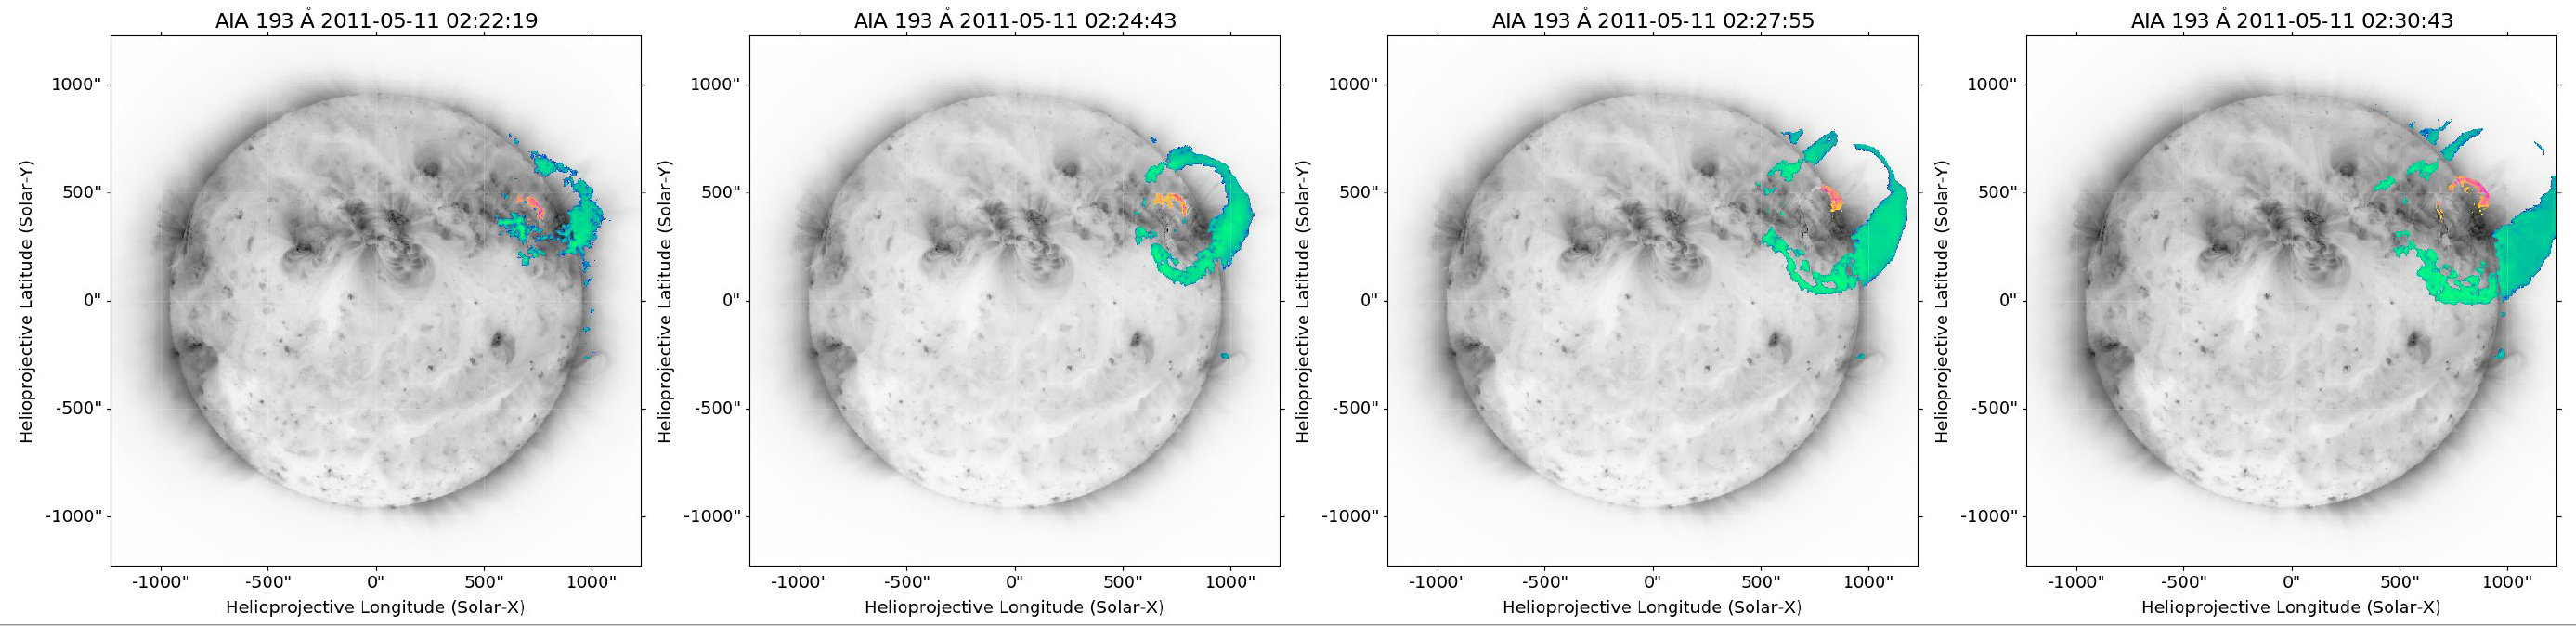
\includegraphics[width=0.9\hsize]{chapter2/figs/fig_1105011_wave_filament_fourpanel_plot.png}
	\caption{Wavetrack images showing progression of a CBF and filament on May 11, 2011. Three snapshots captured \almost2 minutes apart track the CBF and filament over time. Credit goes to \citet{stepanyuk_2022}.}
	\label{fig_wavetrack_cbf_filament}
\end{figure}

\begin{figure}[!htp]
	\centering
	\includegraphics[width=0.7\hsize]{chapter2/figs/wavetrack_figure_110511.png}
	\caption{Wavetrack images of a May 11, 2011 eruption, with CBF mask applied. Four image pairs shown, separated by 2 minutes, to track CBF over time. Credit goes to \citet{stepanyuk_2022}.}
	\label{fig_wavetrack_cbf_center}
\end{figure}

The Wavetrack code was further applied to isolate and study the kinematics of CBFs and filaments in detail. The Fourier Local Correlation Tracking (FLCT) method, extensively utilized for estimating horizontal flows in photospheric magnetograms, was employed for this purpose. Initially proposed as a cross-correlation technique for precise motion measurement, FLCT calculates a 2D flow field that best resembles the scalar field between two consecutive 2D maps.

Figure~\ref{fig_wavetrack_cbf_center} displays four pairs of consecutive AIA images from the May 11, 2011 event, used as input for the FLCT algorithm. Each pair, separated by 24 seconds, is strategically chosen to observe the CBF progression over 6 minutes. The corresponding FLCT results, presented in Figure~\ref{fig_flct_110511}, show the instantaneous plane-of-sky direction of motion and speed of each CBF region. Notably, the results reveal the uneven expansion of the CBF from the central source. In this event, the thinnest part of the CBF, strongly driven by the erupting filament, exhibited the fastest motion compared to other regions on the disk and off the limb. This nuanced information, not discernible from intensity observations alone, underscores the value of our combined Wavetrack and FLCT approach in elucidating the dynamic behavior of coronal features.

\begin{figure}[!htp]
	\centering
	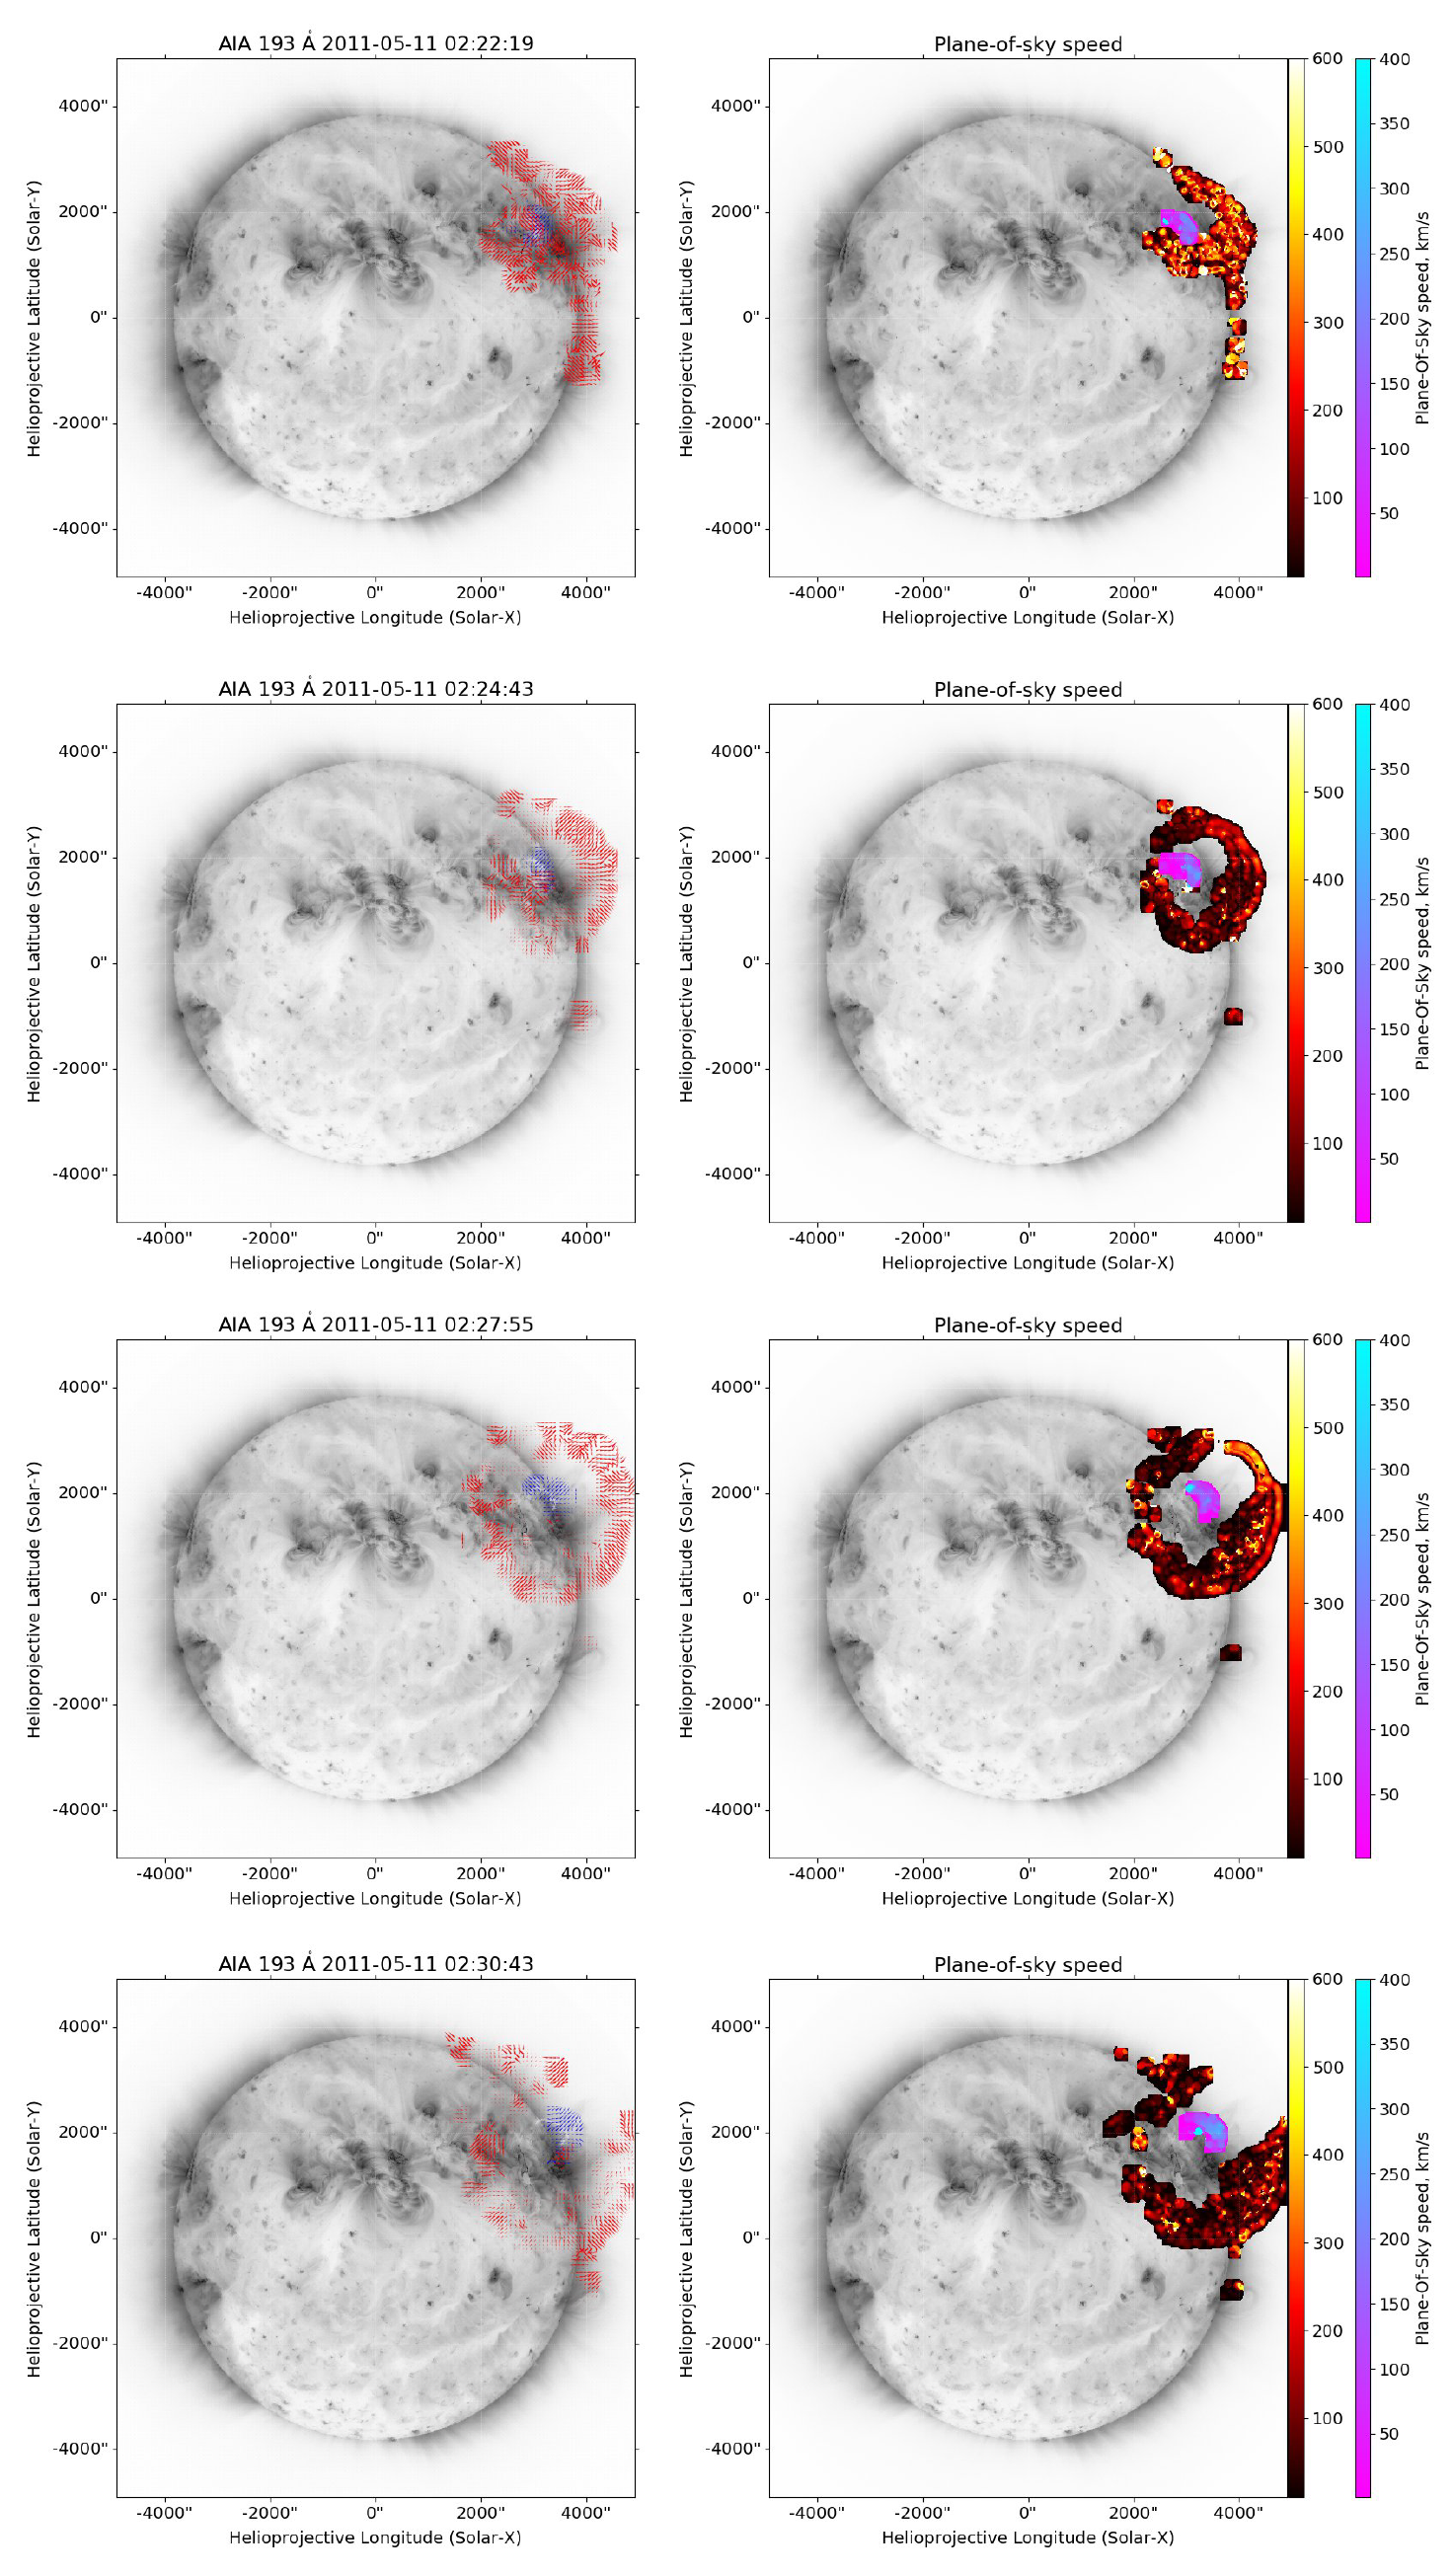
\includegraphics[width=0.7\hsize]{chapter2/figs/flct_wave_filament_doubleplot_figure_110511.png}
	\caption{FLCT model output for four image pairs from Fig. 3. Left: the plane-of-sky velocity vectors. Right: plane-of-sky speed. Credit goes to \citet{stepanyuk_2022}.}
	\label{fig_flct_110511}
\end{figure}

In Figure~\ref{fig_wavetrack_center_of_mass}, the kinematics of the centers of mass (CM) and geometric centers (GC) of the Coronal Bright Front (CBF) were thoroughly analyzed. The research provided detailed metrics over time, including X-axis and Y-axis positions measured from the projected solar center in solar radii, radial distances in \rsun, and radial speeds of the GC and CM points in kilometers per second. The angle between the position vectors of GC and CM, denoted as $\theta(GC-CM)$, was also calculated in degrees. The results illustrated a clear split between the radial positions of GC and CM, with a noticeable shift to the south of the CM after 02:26 UT. This shift was supported by the evolution of the angle $\theta(GC-CM)$, indicating a gradual increase in the wave's thickness in the southwest of the front. Despite these positional changes, the speeds of the GC and CM points varied only slightly, ranging from 0 to 100 \kms. Additionally, the kinematics of the center of mass and geometric centers for the May 11, 2011 event are depicted, showcasing the X-, Y-, and R-positions, distance magnitudes, and angle variations between the two points over time. These findings offer valuable insights into the dynamic behavior and evolution of the CBF during the specified solar event.

\begin{figure}[!htp]
	\centering
	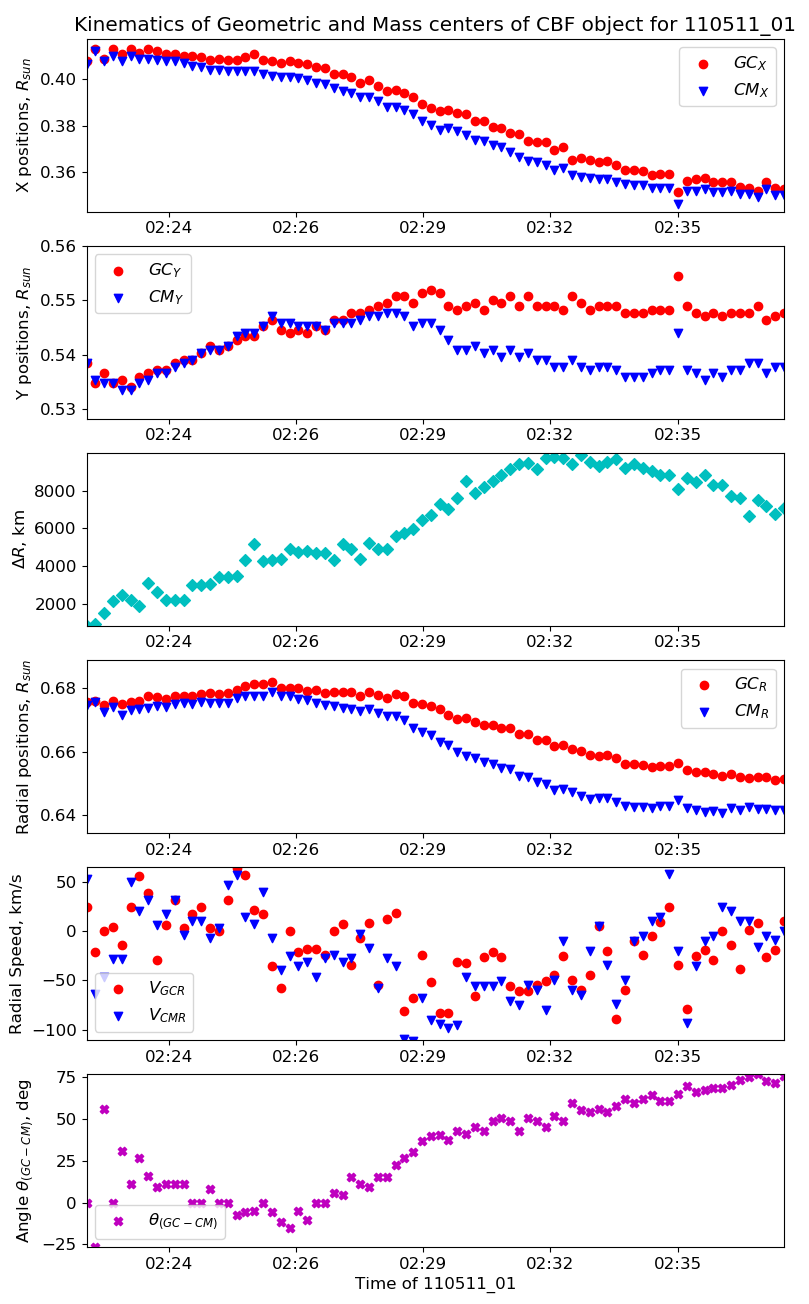
\includegraphics[width=0.7\hsize]{chapter2/figs/event_110511_01_centers_of_mass.png}
	\caption{Analysis of the center of mass and geometric centers' motion during the May 11, 2011 event. The different rows present the X-, Y-, and R- positions for both GC and CM, the distance between GC and CM in kilometers, and the angle between these two points over time. Credit goes to \citet{stepanyuk_2022}.}
	\label{fig_wavetrack_center_of_mass}
\end{figure}

%%%%%%%%%%%%%%%%%%%%%%%%%%%%%%%%%%%%%%%%%%%%%%%%%%%%%%%%%%%%%%%%%%%%%%%%%%%%%%%%%%%%%%%%

\section{Geomagnetic Storms: CME Speed De-Projection vs. In Situ Analysis}
This study, led by \citet{miteva_2023}, examines the relationship between the intensity of geomagnetic storms (GS) and parameters of solar and interplanetary phenomena. We utilize the recently developed PyThea framework to reconstruct the 3D geometry of geo-effective CMEs and compare on-sky and de-projected values, focusing on the reliability of the de-projection capabilities. Spheroid, ellipsoid, and graduated cylindrical shell models are used. We collected parameters of the GS-associated phenomena. Considerable variation in 3D de-projections of CME speeds was obtained depending on the reconstruction model chosen and subjective observations. Fast CME speeds combined with frontal magnetic structure orientation when reaching Earth's magnetosphere proved the best indicator of GS strength. More accurate estimations of geometry, direction, and de-projected speeds are critical for operational GS forecasting in space weather prediction schemes.

\subsection{Overview}
Solar eruptive events like CMEs and solar flares (SFs) can generate disturbances that propagate through interplanetary space and impact Earth's magnetosphere, leading to space weather effects \citep{fletcher_2011, webb_2012, klein_2017, temmer_2021}. The electromagnetic radiation from SFs arrives at Earth first, followed by energetic particles. The plasma clouds of CMEs take longer, from tens of hours up to a few days, to impact Earth's environment \citep{malandraki_2018, gopalswamy_sun_sw_2022}. The temporary disruption of Earth's magnetosphere and atmosphere due to these solar events are known as geomagnetic storms (GSs) \citep{gonzalez_1994, saiz_2013, lakhina_2016}.

The coupling between solar wind plasma and Earth's magnetosphere occurs through magnetic reconnection, enabled when the interplanetary (IP) magnetic field turns southward (negative $B_z$ component) and impacts Earth at high speed, as during CMEs \citep{dungey_1961, akasofu_1981, echer_2022}. This leads to increased particle injection into the magnetosphere and atmosphere, causing bright auroral displays. Drifting electrons and protons also drive the westward ring current responsible for decreases in the horizontal magnetic field measured by the disturbance storm time (Dst) index \citep{gonzalez_1994, saiz_2013, lakhina_2016}.

Fast CMEs propagating through IP space (ICMEs) cause the most intense GSs, with sudden Dst decreases, compared to gradual storms from corotating interaction regions (CIRs) \citep{tsurutani_1997, zhang_2007, wu_2016, borovsky_2006}. ICME shock waves and magnetic ejecta produce cascading effects in near-Earth space that can disrupt technology \citep{pulkkinen_2007}.

Earth-directed fast ejecta with strong southward magnetic fields inside are the most geoeffective. However, single spacecraft observations are limited by projection effects, leading to uncertain CME speed estimations \citep{paouris_2021, kouloumvakos_2022}. Previous studies found no clear relationship between GS intensity and solar flare parameters or CME properties like projected speed and angular width \citep{samwel_2023}. Furthermore, CME magnetic structure cannot be derived from remote sensing data. Reliable solar or near-Sun measurements that provide early warnings for potential GS strength remain lacking.

Accurately predicting when an incoming disturbance will impact Earth requires determining the arrival time and speed of CMEs. Different portions of these large structures, such as the apex or flanks, can hit Earth upon arrival at 1 AU. Flank hits may only involve the CME sheath while apex hits include both sheath and ejecta, leading to different magnetospheric effects \citep{kay_2018}. Therefore, deducing CME directionality and 3D geometry is important. To maximize forecast lead time, these parameters should be estimated as early as possible when the CME emerges in coronagraph fields of view. In images, CMEs appear as line-of-sight integrated brightness enhancements projected onto the observing plane \citep{vourlidas_2003, jackson_2010}.

Further developing reconstruction techniques to correct for projection effects can improve CME propagation understanding and impact forecasting \citep{thernisien_2009, mierla_2010, wood_2010, thernisien_2011}. Several CME propagation models exist \citep{odstrcil_2004, xie_2004, vrvsnak_2013, pomoell_2018}. A study found 2D CME speeds underestimate 3D speeds by \almost20\% while 2D widths overestimate 3D widths \citep{jang_2016}. Another study showed observer bias in 3D modeling using graduated cylindrical shells, even for experienced observers \citep{verbeke_2022}. CME structure interpretation differs, and line-of-sight integration leads to non-unique solutions.

This study focuses on deducing CME directionality and near-Sun speeds using new tools like PyThea \citep{kouloumvakos_2022}. We analyze geo-effective cycle 24 CMEs using multiple reconstruction techniques by two team members. Comparisons are made between derived parameters and Dst. CME speed correlations with ICME and IP shock speeds evaluate 3D de-projection value for arrival forecasting. Other IP parameters are also examined, including shock speed, plasma jumps, and magnetic fields near L1. We examine the correlation between the intensity of geomagnetic storms and parameters of solar and interplanetary phenomena. More specifically, we focus on the speed and geometry of CMEs, as well as interplanetary shocks, as these factors are known to play a significant role in the occurrence and intensity of geomagnetic storms. The objective of the study is to analyze the correlations between the intensity of GS and parameters of solar and IP phenomena. The study also aims to perform 3D geometry reconstructions of geo-effective CMEs using the PyThea framework and compare the de-projected CME speeds with in situ data.

%\subsection{Data Analysis and Methods}
The event selection process for this investigation commenced with the identification of significant GSs within Solar Cycle 24 (SC24). These storms were characterized by a Dst index exceeding 100 nT, as per the classification outlined in \citet{gonzalez_1994}. A total of 25 GSs were identified, with Dst indices ranging from 101 to 234 nT. Previous studies have explored the solar and IP origins of these GSs in SC24 \citep{gopalswamy_gs_2022, qiu_2022, besliu_2022, abe_2023}. However, the comprehensive review of all pertinent literature falls beyond the purview of this study. It is noteworthy that SC24 exhibited a reduced number of GSs in comparison to preceding solar cycles \citep{selvakumaran_2016}.

In our investigation, distinct from prior analyses, our objective was to establish a causal connection between the identified GSs and potential IP and/or solar phenomena. This approach mirrors methodologies employed by other researchers \citep{zhang_2007, gonzalez_2007, gopalswamy_2008, echer_2013, manu_2022}. To delineate the solar and IP drivers, we employed an association procedure widely acknowledged in the field of Space Weather (SW) research. The methodology involves searching for the IP and solar origins of a GS storm within a specific timeframe preceding the reported GS occurrence at Earth. The sequential steps of our approach are delineated below:

\begin{enumerate}
	\item \textbf{Temporal Association with IP and ICME Events}:
	We initiated the analysis with a temporal association between the GS and recorded IP shocks in the vicinity of Earth. This association was established within a 1-day period preceding the reported minimum Dst of the GS. A parallel procedure was employed for the association with ICMEs reported in proximity to Earth. Additionally, animations from the \textit{helioweather} archive\footnote{\helioweatherurl} (accessed on 5 April 2023) were utilized to validate potential ICME and IP shock candidates.
	
	\item \textbf{Association with CMEs}:
	Subsequently, we extended the association to include CMEs within a 3-to-5 day window prior to the IP (or GS) timing. Information from available solar and IP event catalogs, as well as animations from the \textit{helioweather} archive\footnotemark[\value{footnote}] (accessed on 5 April 2023), was employed for this purpose.
	
	\item \textbf{Completion of the Association with SFs}:
	The final step involved associating the GS with the identification of a SF linked to the previously associated CME. This association was based on timing (within one hour between the SF onset and CME timing) and location constraints (the SF location had to align with the solar quadrant reported in the measurement position angle, MPA, of the CME).
\end{enumerate}

All utilized databases, catalogs, and publicly available lists pertinent to the analysis are summarized as follows:

\begin{itemize}
	\item GS database (Kyoto)\footnote{\url{https://wdc.kugi.kyoto-u.ac.jp/dstdir/index.html}} (accessed on 5 April 2023);
	\item SF database (GOES)\footnote{\url{http://ftp.swpc.noaa.gov/pub/warehouse/}} (accessed on 5 April 2023);
	\item CME catalog (SOHO-LASCO)\footnote{\url{CME catalog (SOHO-LASCO)}} (accessed on 5 April 2023);
	\item ICME Wind database\footnote{\url{https://wind.nasa.gov/ICME_catalog/ICME_catalog_viewer.php}} (accessed on 5 April 2023);
	\item ICME ACE database\footnote{\url{https://izw1.caltech.edu/ACE/ASC/DATA/level3/icmetable2.htm}} (accessed on 5 April 2023);
	\item IP shock database (Wind)\footnote{\url{http://www.ipshocks.fi/database}},\footnote{\url{https://lweb.cfa.harvard.edu/shocks/wi_data/}} (accessed on 5 April 2023).
\end{itemize}

\subsection{GSs and IP Phenomena}
The findings pertaining to GSs and their associated ICMEs and IP shocks are succinctly presented in Table 1 in \citet{miteva_2023}. The initial column designates the event number (\#), a consistent reference utilized throughout this paper. Columns (2) and (3) detail the GS date, hour (mm-dd/hr), and the corresponding Dst index (in nT). Subsequently, columns (4)–(6) expound upon the ICME parameters \citep{nieves_2018}, drawing from the Wind database accessible at this website\footnote{\url{https://wind.nasa.gov/ICME_catalog/ICME_catalog_viewer.php}}. The sheath duration (D, in hours), representing the temporal span between the initiation times of the ICME and the magnetic structure, is computed from the available timings within the plots offered by the aforementioned Wind database, and is presented in column (7). The ICME in situ measured speed is extracted from both the Wind and ACE databases, with the exception of E11 where no ICME is reported.

Column (8) integrates the minimum Bz component throughout the ICME duration, as ascertained from the data available at this website\footnote{\url{https://cdaweb.gsfc.nasa.gov/}}, thereby enhancing the comprehensiveness of the dataset. In Column (9), we conduct a qualitative assessment of the ICME arrival orientation. Specifically, we visually inspect the intersection point between the ICME structure and Earth using ecliptic plane animations accessible at this website\footnote{\helioweatherurl}. The orientations are denoted as either \textit{hit} (nose) or \textit{f} (flank) arrivals. Instances of discrepancies among diverse data sources, such as the presence of solar wind streams or CIRs visible in animations contradicting ICME arrivals identified through in situ data, are marked as 'u' (uncertain) in the same column. This classification signifies situations where a distinct ICME structure propagating through the IP space could not be conclusively observed. Noteworthy is the occurrence of swift solar wind flows and/or CIRs recorded near Earth during ICME and/or shock wave events. For instance, in the cases of E11 and E18, a CIR was identified as their IP origin by \citet{qiu_2022}; however, in contrast to these findings, our methodology does not differentiate between ICME and sheath origins.

The final columns, (10)–(13), enumerate the properties of the IP shock, incorporating timing, speed, magnetic field, density, temperature jump at the shock interface, and the Mach number (Mms). These details are sourced from Wind satellite data, available at this website\footnote{\url{http://www.ipshocks.fi/database}}, with the exception of E24, where the median shock speed is derived from this website\footnote{\url{https://lweb.cfa.harvard.edu/shocks/wi_data/}}. Notably, for E17, E18, and E25, no IP shocks are reported in either database.

\subsection{GSs and Solar Phenomena}
In the context of five cases denoted as E05, E11, E17, E18, and E22, our attempts to identify SFs or Coronal Mass Ejections (CMEs) were unsuccessful. Furthermore, in an additional six cases, the specification of SFs proved unattainable. The ensuing presentation provides details on the parameters of the remaining cases, specifically focusing on the solar origins associated with GSs, as outlined in Table~\ref{tab_GS_sol}.

Columns (2)–(5) of Table~\ref{tab_GS_sol} elucidate the properties of the GS-associated SFs, while columns (6) to (9) furnish the parameters of the GS-associated CMEs. The identified SFs exhibit a range of magnitudes from C1.2 to X5.4 and are predominantly positioned proximate to the solar disk center, with the exception of E02 and E03. The CMEs associated with these events possess on-sky projected speeds, denoted as 2D, spanning from 126 to 2684 \kms, extracted from the SOHO-LASCO CDAW catalog. Notably, the majority of the GS-associated CMEs (15 out of 20) exhibit a halo configuration, while three others are in close proximity to halo.

It is imperative to note that events with uncertain CME origins have been excluded from the subsequent 3D analyses. Specifically, in the case of E07, the unique orientation of the double CME rendered the de-projection procedure unfeasible for the same CME structure, leading to its exclusion from the 3D analyses. Additionally, for seven other cases (E12, E14–E16, E19, E23, E25), the online tool utilized for analyses failed to retrieve data simultaneously from both spacecraft. Consequently, these cases have also been omitted from the 3D analyses.

For the remaining 12 cases, successful 3D CME speed reconstructions were achieved from each model. The mean values, based on 2 or 4 available fits (as detailed in the subsequent subsection), are presented in the concluding columns (10)–(12) of Table~\ref{tab_GS_sol}. This comprehensive overview provides a foundation for the subsequent analytical discussions, offering a detailed characterization of the solar events associated with the studied GSs.

\subsection{PyThea 3D De-Projection Tool}
The de-projection methodology employed in this investigation relies on the innovative PyThea online tool designed for the 3D reconstruction of CMEs and shock waves \citep{kouloumvakos_2022}. All three available models within PyThea, namely spheroid, ellipsoid, and the graduated cylindrical shell (GCS), are applied in this study. The fitting procedure is conducted independently by two observers within our team. Figure~\ref{fig_3D_fit} presents an illustrative example of the fits for event E03.

\begin{figure}[!htp]
	\centering
	\begin{subfigure}[b]{0.3\textwidth}
		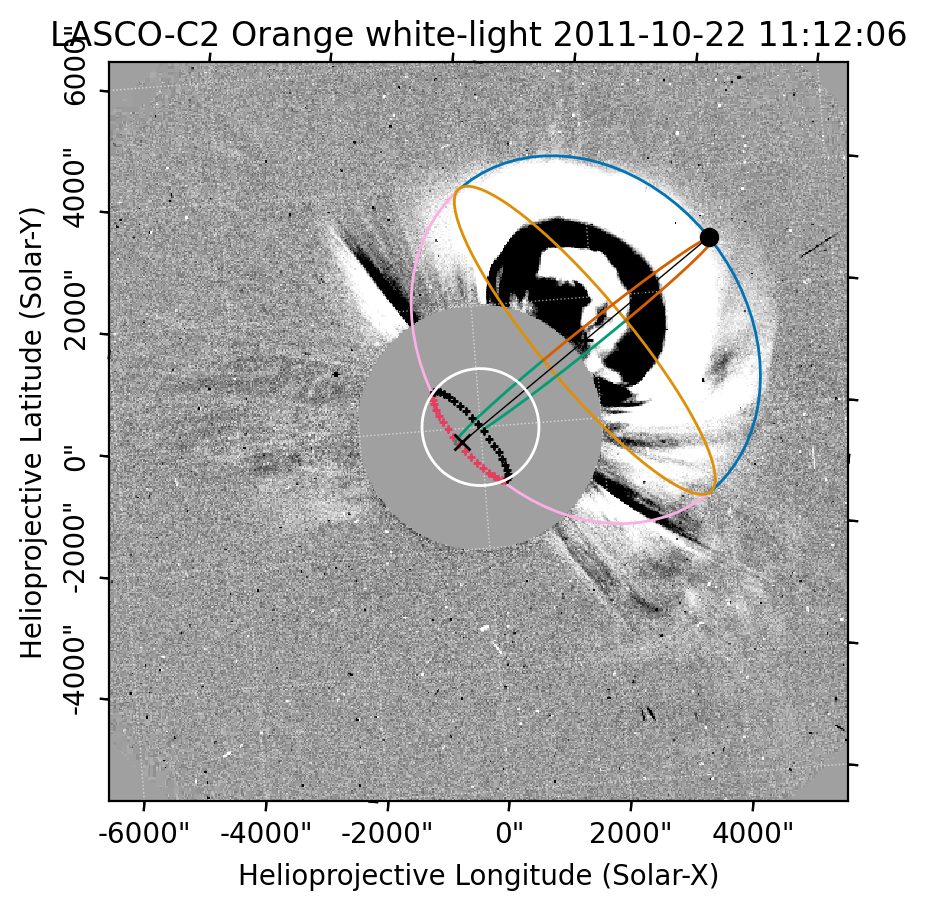
\includegraphics[width=\textwidth]{chapter2/figs/Fig_s1.png}
	\end{subfigure}
	\hfill
	\begin{subfigure}[b]{0.3\textwidth}
		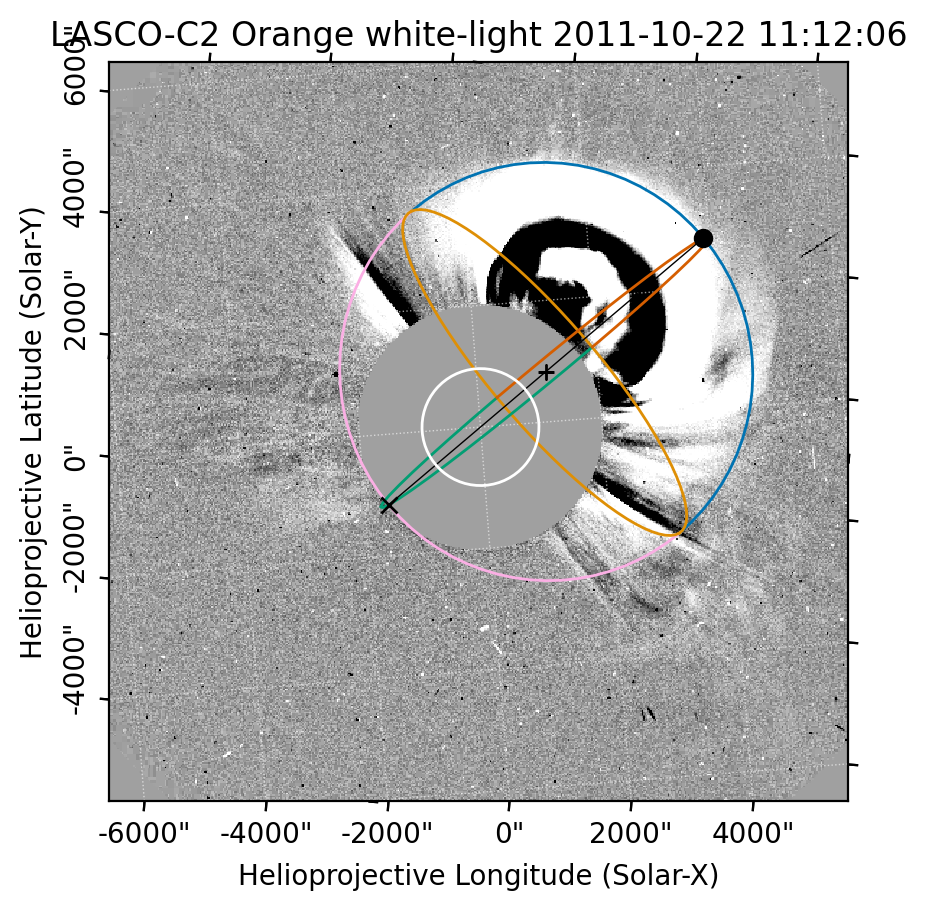
\includegraphics[width=\textwidth]{chapter2/figs/Fig_e1.png}
	\end{subfigure}
	\hfill
	\begin{subfigure}[b]{0.3\textwidth}
		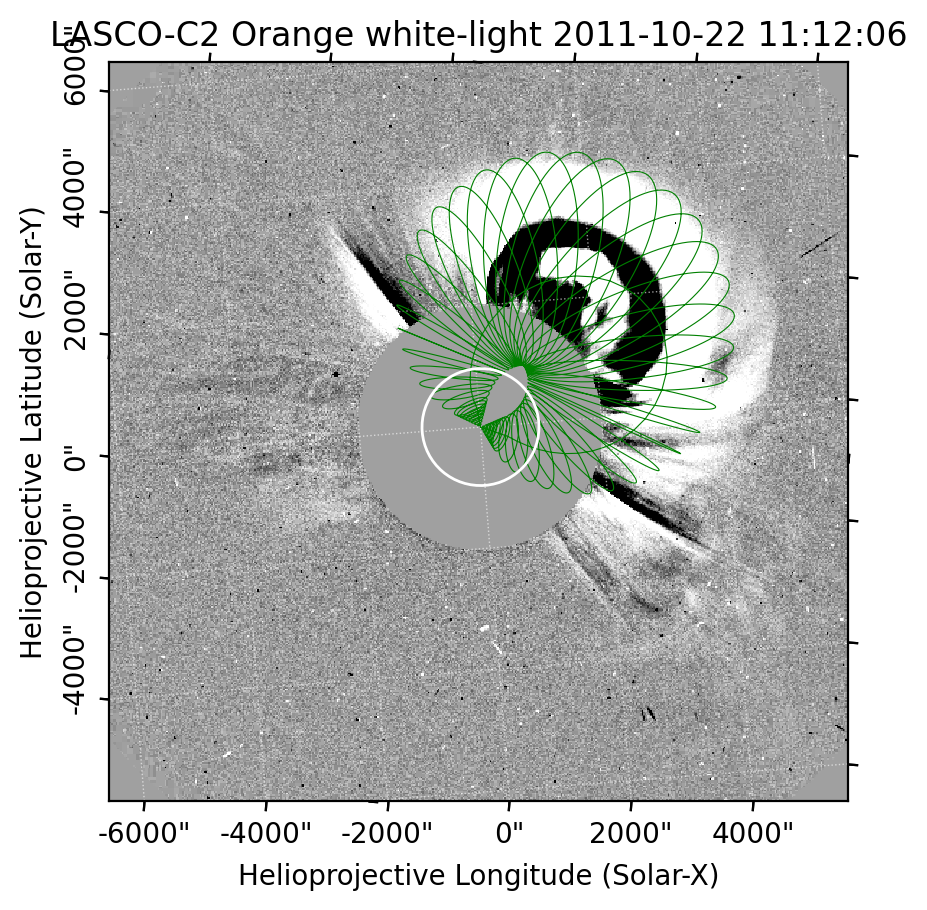
\includegraphics[width=\textwidth]{chapter2/figs/Fig_g1.png}
	\end{subfigure}
	\medskip % Add some vertical space between rows
	\begin{subfigure}[b]{0.3\textwidth}
		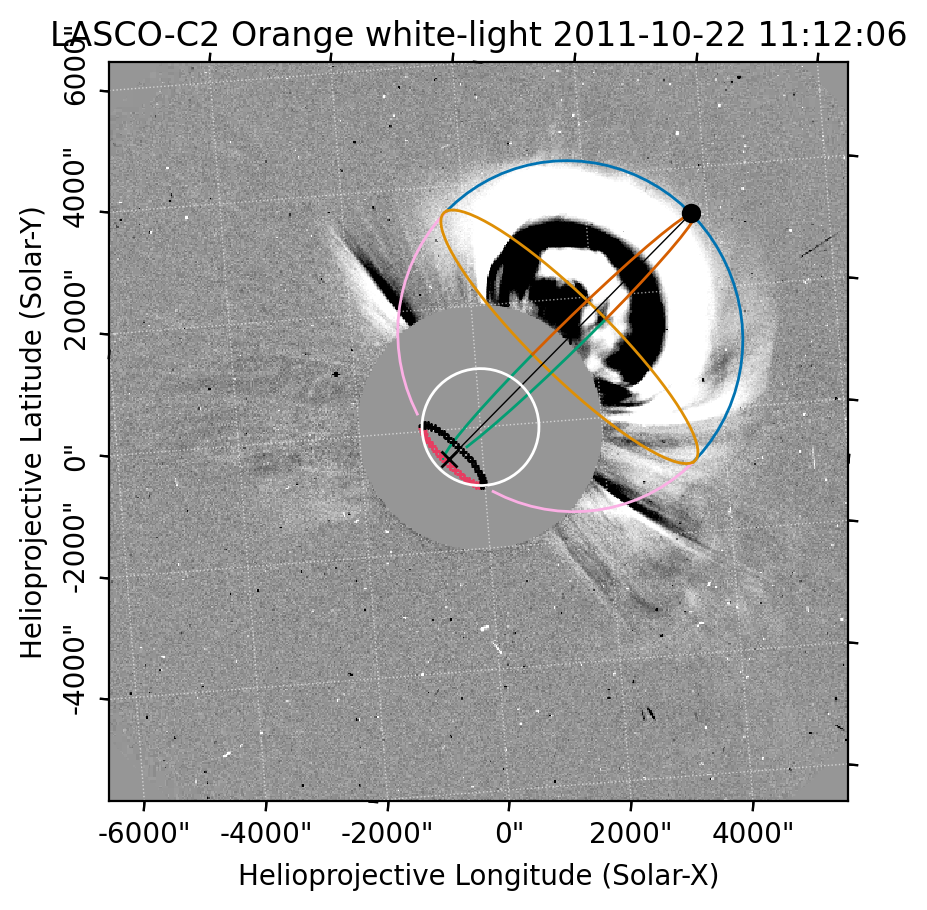
\includegraphics[width=\textwidth]{chapter2/figs/Fig_s2.png}
	\end{subfigure}
	\hfill
	\begin{subfigure}[b]{0.3\textwidth}
		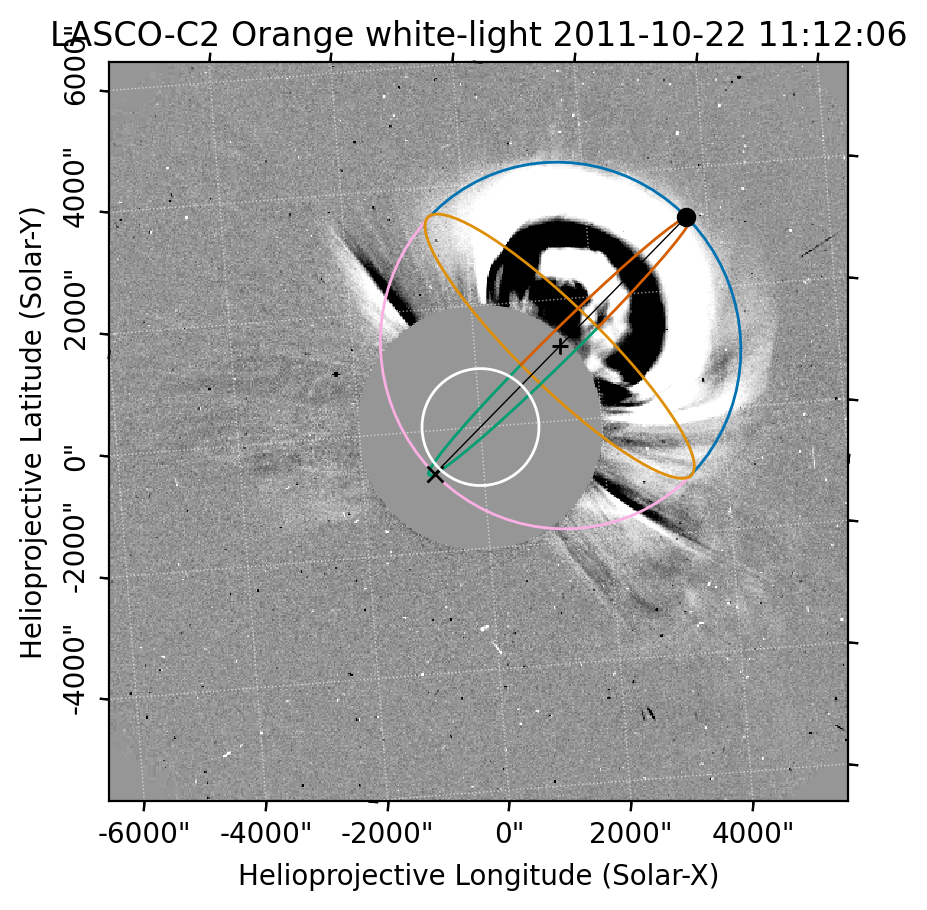
\includegraphics[width=\textwidth]{chapter2/figs/Fig_e2.png}
	\end{subfigure}
	\hfill
	\begin{subfigure}[b]{0.3\textwidth}
		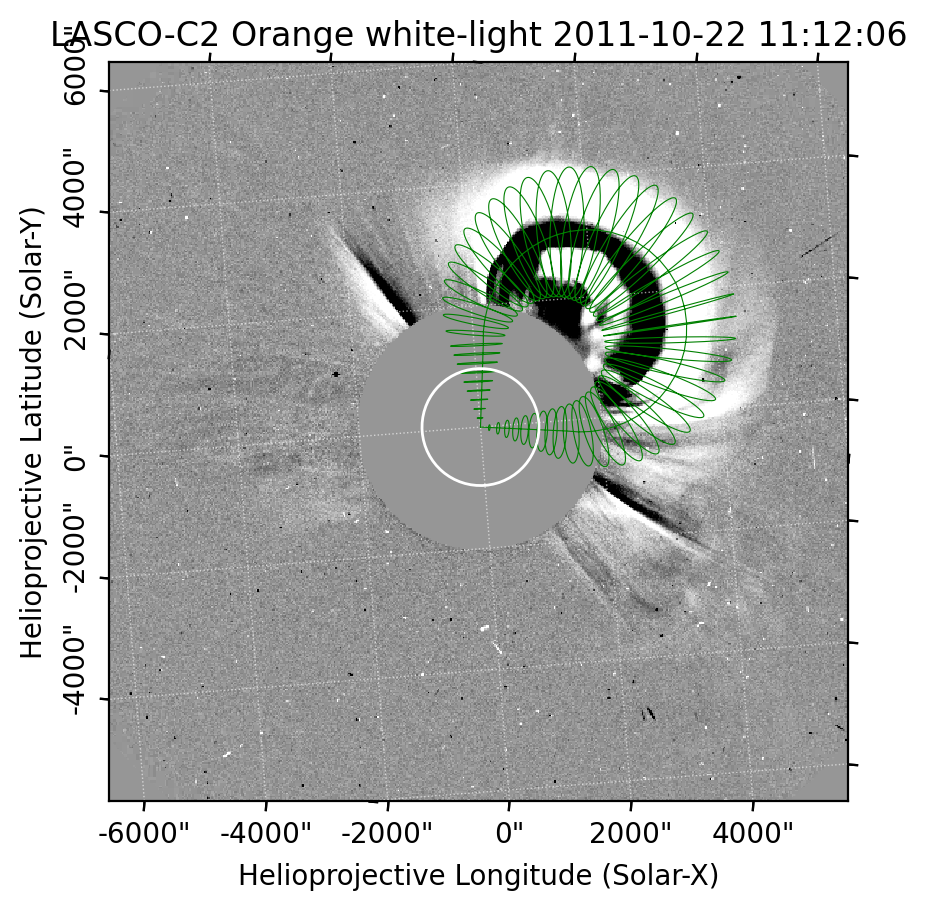
\includegraphics[width=\textwidth]{chapter2/figs/Fig_g2.png}
	\end{subfigure}
	\caption{3D reconstructions of a CME (E03) using the spheroid, ellipsoid, and GCS model from the PyThea tool performed by observers 1 and 2 (top and bottom row, respectively). Credit goes to \citet{miteva_2023}.}
	\label{fig_3D_fit}
\end{figure}

Upon scrutinizing the fitting outcomes for this particular example, it becomes evident that the reconstructions exhibit a discernible bias. The observer's subjective \textit{choice} of structures to align with the model introduces a level of variability. In the top row of Figure~\ref{fig_3D_fit}, distinct shock-related structures (manifested as the bending of streamers) are observed, upon which the idealized GCS flux rope geometry is fitted. Consequently, there is a likelihood of overestimating the CME width. Despite this bias, it is noteworthy that the overall results, including directivity and speed for event E03, are minimally impacted. However, it is acknowledged that the complexity of structure choices can lead to larger discrepancies among different observers.

This study places emphasis on deriving de-projected CME speeds based on fits conducted at two distinct time steps. For each of the three models, the initial CME longitude and latitude are manually specified, utilizing the provided locations of the CME-accompanied SFs. It is important to note that these values exhibit minimal to no substantial changes post-finalization of the fitting procedure. Consequently, the final CME directivity provided by PyThea is considered to be a relatively crude estimate. The ultimate orientations of the CME in IP space and at Earth are derived solely from qualitative information extracted from animations available at this website\footnote{\helioweatherurl}. This approach ensures a rigorous and consistent basis for evaluating the de-projected CME speeds in our analyses.

\subsection{Results}
\subsubsection{Projection Effects}
In our investigation, a fitting analysis of approximately 10 CMEs was undertaken by two designated observers within our research team, I was one of the observers. This analysis involved the utilization of all three models available in the PyThea framework, each selected based on the evaluators' individual considerations.

To elucidate, the fitting process was executed at two distinct time steps to derive a velocity parameter based on the height–time estimation. For each specific event, both observers iteratively conducted the 3D de-projection procedure twice, resulting in averaged values for the CME speeds. These values are meticulously presented in Table~\ref{tab_fits}, rounded to the nearest tenth. The disparity between these two fitting instances is denoted as an error (or uncertainty), spanning from 10 \kms to twice the estimated speed. Additionally, Figure 2 illustrates the correlation between 3D speeds and the corresponding estimated errors for each observer. Notably, considerable variability is observed in both plots, particularly concerning the GCS model; nonetheless, a discernible positive trend emerges between the estimated error magnitude and the CME speed.

The inherent subjectivity and diverse levels of experience among observers play a crucial role in the visual fitting procedure. Noteworthy distinctions in evaluated speeds are evident not only between individual observers using the same model (e.g., spheroid fit for E06) but also between a single observer applying different models (e.g., spheroid and GCS for E13). Furthermore, variations in operating system software further contributed to differences in results. Notably, events E04, E08, and E21 were not completed by both observers due to either PyThea computing resource failures or the substantial uncertainty associated with the visual assessment of CME structures.

Our findings underscore the well-established subjectivity inherent in procedures relying on personal judgment for fit quality, where the alignment of structures with the model is subjective. A more comprehensive explanation of this human-in-the-loop bias is detailed in \citep{verbeke_2022}. The specific values of CME speeds are meticulously outlined in Table~\ref{tab_fits}, while their averaged values, categorized by model, as determined by both observers, are presented in Table~\ref{tab_GS_sol}. These averaged values will serve as the basis for subsequent correlation studies.

\begin{landscape}
	\footnotesize
	\begin{longtable}{ccccccccccccc}
		\caption{Characteristics of GSs, ICMEs, and IP Shock Waves. Magnetic Obstacle (MO) categorized as Flux-rope (Fr), Small rotation flux-rope (F-), Large rotation flux-rope (F+), Complex (Cx), or Ejecta (E). The timestamp includes month (mm), day (dd), and time (UT). Dst is measured in nT, speed in \kms, $\Delta$ (duration from ICME start to MO start) in hours, $B_z$ in nT, hit locations denoted as n (nose), f (flank), */** (fast/slow speed), u (streamer/no clear ICME). {\bf Additional abbreviations:} $X$: magnetic field/plasma density/temperature; d/u: downstream/upstream side of the shock interface; $M_{\rm ms}$: Mach number. Credit goes to \citet{miteva_2023}.}
		\label{tab_GS_IP}\\
			\toprule
			\textbf{\#}	& \multicolumn{2}{c}{\textbf{GS}} & \multicolumn{6}{c}{\textbf{ICME parameters}} & \multicolumn{4}{c}{\textbf{IP shock parameters}} \\
			& mm-dd/hr & Dst & mm-dd/time & type & speed Wind/ACE & $\Delta$ & $B_z$ & hit & mm-dd/time & speed & $X_d/X_u$ & $M_{\rm ms}$ \\
			(1) & (2) & (3) & (4) & (5) & (6) & (7) & (8) & (9) & (10) & (11) & (12) & (13)\\
			\midrule
			\textbf{2011}\\
			E01	& 08-06/04 & $-$115 & {\it 08-06/22:00} & - & -/540 & - & $-$22.8 & f* & 08-05/18:41 & 789 & 2.52/1.37/2.21 & 3.7 \\
			E02	& 09-26/24 & $-$118 & {\it 09-26/22:00} & - & -/580 & - & $-$33.6 &  f & 09-26/11:44 & 544 & 2.35/2.56/2.64 & 2.4 \\
			E03	& 10-25/02 & $-$147 & 10-24/17:41 & Cx & 483/460 & 6.7 & $-$24.6 &  f & 10-24/17:40	& 542 & 2.16/2.94/4.88 & 2.5 \\
			\textbf{2012} \\
			E04 & 03-09/09 & $-$145 & 03-08/10:32 & Cx & 576/550 & 9.4 & $-$19.2 &  n & 03-08/10:31 & 1245 & 1.42/1.31/1.25 & 8.4 \\
			E05 & 04-24/05 & $-$120 & 04-23/02:15 & F- & 373/370 &  14.6 & $-$15.9 &  f & 04-23/02:15 & 416 & 2.45/2.44/1.87 & 1.7 \\
			E06 & 07-15/17 & $-$139 & 07-14/17:39 & Fr & 491/490 & 12.6 & $-$20.0 &  n & 07-14/17:39 & 617 & 2.08/2.53/4.29 & 3.3	\\
			E07	& 10-01/05 & $-$122 & 09-30/10:14 & Cx & 354/370 & 2.0 & $-$21.2 &  f & 09-30/22:19	& 452 & 2.55/2.00/2.05 & 2.5 \\ 
			E08	& 10-09/09 & $-$109 & 10-08/04:12 & Fr & 398/390 & 11.6 & $-$16.0 &  u & 10-08/04:12 & 445 & 1.96/2.01/1.63 & 1.7 \\
			E09	& 11-14/08 & $-$108 & 11-12/22:12 & F+ & 381/380 &  10.2  & $-$20.6 &  f & 11-12/22:12 & 386 & 2.18/2.20/1.08 & 1.6	\\
			\textbf{2013}\\
			E10 & 03-17/21 & $-$132 & 03-17/05:21 & Fr & 529/520 & 8.8 & $-$19.3 &  n & 03-17/05:22 & 719 & 2.45/2.68/10.5 & 4.1 \\ 
			E11 & 06-01/09 & $-$124 & - & - & -/- & - & $-$8.8 &   u & 05-31/15:12 & 410 & 2.90/2.16/2.83 & 2.1 \\
			E12	& 06-29/07 & $-$102 & 06-27/13:51 & Fr & 391/- & 12.5 & $-$12.4 &  u & 06-30/10:42 & 349 & 1.55/1.61/1.27 & 1.4 \\
			\textbf{2014} \\
			E13	& 02-19/09 & $-$119 & 02-18/05:59 & Fr & 421/520 & 9.1 & $-$15.4 &  u & 02-19/03:10 & 597 & 1.82/1.69/1.51 & 1.9 \\
			\textbf{2015}\\
			E14	& 01-07/12 & $-$107 & 01-07/05:38 & F+ & 451/450 & 0.8 & $-$20.4 &  u & 01-07/05:39 & 494 & 1.70/1.73/1.89 & 1.2 \\
			E15 & 03-17/23 & $-$234 & {\it 03-17/13:00} & - & -/560 & - & $-$26.0 &  f* & 03-17/04:00 & 562 & 2.52/2.43/3.50 & 2.6	\\ 
			E16 & 06-23/05 & $-$198 & 06-22/18:07 & Cx & 598/610 &  8.3 & $-$39.0 &  n & 06-22/18:08 & 767 & 3.34/3.63/6.70 & 4.1	\\
			E17	& 09-09/13 & $-$105 & 09-07/13:05 & F+ & 468/460 & 10.4 & $-$12.6 &  u & - & - & - & -\\ 
			E18	& 10-07/23 & $-$130 & 10-06/21:35 & Fr & 425/- & 0 &  $-$9.2 & u & - & - & - & - \\ 
			E19	& 12-20/23 & $-$166 & 12-19/15:35 & Fr & 398/400 & 22.1 & $-$19.0 &  n & 12-19/15:38 & 563 & 2.49/2.25/4.87 & 3.0 \\ 
			\textbf{2016} \\
			E20	& 01-01/01 & $-$116 & {\it 12-31/17:00} & - & -/440 & - & $-$16.3 &   n** & 12-31/00:18 & 404 & 2.20/2.27/3.99 & 2.6 \\
			E21	& 01-20/17 & $-$101 & 01-19/03:31 & Fr & 362/370 & 7.9 & $-$11.6 &  f & 01-18/21:21 & 350 & 1.73/1.91/1.60 & 1.7 \\ 
			E22	& 10-13/18 & $-$110 & 10-12/21:37 & F+ & 384/390 &  8.8 &  $-$6.9 &  u & 10-12/21:16	& 431 & 1.82/2.47/4.43 & 1.9 \\
			\textbf{2017}\\
			E23	& 05-28/08 & $-$125 & 05-27/13:45 & F+ & 318/360 & 9.1 & $-$20.2 &  f & 05-27/14:42 & 378 & 2.68/2.94/2.95 & 1.9	\\ 
			E24	& 09-08/02 & $-$122 & 09-07/16:17 & E & 683/460 &  8.0  & $-$32.2 &  f* & 09-07/{\it 22:28} & {\it 718} & - & - \\
			\textbf{2018}\\
			E25	& 08-26/07 & $-$175 & 08-25/01:02 & F+ & 406/410 & 11.0 & $-$6.8 &  n & - & - & - & - \\ 
			\bottomrule
		\end{longtable}
\end{landscape}

\begin{table}[!htp]
	\tiny
	\caption{Parameters of the solar origin, SFs, and CMEs for GSs from Table~\ref{tab_GS_IP}. All times are in UT, speeds in \kms, AW and MPA in degrees. Credit goes to \citet{miteva_2023}.}
	\label{tab_GS_sol}
	\begin{adjustbox}{width=\textwidth}
		\begin{tabular}{@{}cccccccccccc@{}}
			\toprule
			\textbf{\#}	& \multicolumn{4}{c}{\textbf{SF parameters}} & \multicolumn{4}{c}{\textbf{2D CME parameters}} & \multicolumn{3}{c}{\textbf{3D CME speed}} \\
			& mm-dd & class & onset & location & time & speed & AW & MPA & spheroid & elliptical & GCS  \\
			(1) & (2) & (3) & (4) & (5) & (6) & (7) & (8) & (9) & (10) & (11) & (12)  \\
			\midrule
			\textbf{2011}\\
			E01 & 08-04 & M9.3 & 03:41 & N19W36 & 04:12 & 1315 & 360 & 298 & 1990 & 1920 & 1780 \\
			E02 & 09-24 & M7.1 & 12:33 & N10S56 & 12:48 & 1915 & 360 & 78 & 1570 & 1590 & 1720 \\
			E03 & 10-22 & M1.3 & 10:00 & N25W77 & 10:24 & 1005 & 360 & 311 & 760 & 690 & 840 \\
			\textbf{2012} \\
			E04 & 03-07 & X5.4 & 00:02 & N17S27 & 00:24 & 2684 & 360 & 57 & 2150 & 2460 & 2530 \\
			E05 & \multicolumn{8}{c}{uncertain origin} & - & - & -\\
			E06 & 07-12 & X1.4 & 15:37 & S15W01 & 16:48 & 885 & 360 & 158 & 1060 & 1780 & 1520 \\
			E07 & 09-28 & C3.7 & 23:36 & N06W34 & 24:12 & 947 & 360 & 251 & \multicolumn{3}{c}{multiple CMEs}\\
			E08 & 10-05 & \multicolumn{3}{c}{uncertain} & 02:48 & 612 & 284 & 202 & 350 & 360 & 350 \\
			E09 & 11-09 & \multicolumn{3}{c}{uncertain} & 15:12 & 559 & 276 & 157 & 660 & 570 & 720 \\
			\textbf{2013}\\
			E10 & 03-15 & X1.1 & 05:46 & N11S11 & 07:12 & 1063 & 360 & 112 & 720 & 1040 & 1110 \\
			E11 & \multicolumn{8}{c}{uncertain origin} & - & - & -\\
			E12 & 06-28 & \multicolumn{3}{c}{uncertain} & 02:00 & 1037 & 360 & 214 & \multicolumn{3}{c}{no SOHO images}\\
			\textbf{2014} \\
			E13 & 02-16 & M1.1 & 09:20 & S11E01 & 10:00 & 634 & 360 & 227 & 340 & 690 & 890 \\
			\textbf{2015}\\
			E14 & 01-03 & C1.2 & 03:06 & S05E21 & 03:12 & 163 & 153 & 144 & \multicolumn{3}{c}{no STEREO images} \\
			E15 & 03-15 & C9.1 & 01:15 & S22W25 & 01:48 & 719 & 360 & 240 & \multicolumn{3}{c}{no STEREO images} \\
			E16 & 06-21 & M2.6 & 02:06 & N12E13 & 02:36 & 1366 & 360 & 72 & \multicolumn{3}{c}{no STEREO images} \\
			E17 & \multicolumn{8}{c}{uncertain origin} & - & - & - \\
			E18 & \multicolumn{8}{c}{uncertain origin} & - & - & - \\
			E19 & 12-16 & C6.6 & 08:34 & S13W04 & 09:36 & 579 & 360 & 334 & \multicolumn{3}{c}{no STEREO images} \\
			\textbf{2016} \\
			E20 & 12-28 & M1.8 & 11:20 & S23W11 & 12:12 & 1212 & 360 & 163 & 820 & 680 & 1080 \\
			E21 & 01-14 & \multicolumn{3}{c}{uncertain} & 23:24 & 191 & 360 & 234 & 620 & 440 & 280 \\
			E22 & \multicolumn{8}{c}{uncertain origin} & - & - & - \\
			\textbf{2017}\\
			E23 & 05-23 & \multicolumn{3}{c}{uncertain} & 05:00 & 259 & 243 & 281 & \multicolumn{3}{c}{no SOHO images}\\
			E24 & 09-04 & M5.5 & 20:28 & S11W16 & 20:36 & 1418 & 360 & 184 & 1020 & 1290 & 990 \\
			\textbf{2018}\\
			E25 & 08-20 & \multicolumn{3}{c}{uncertain} & 21:24 & 126 & 120 & 266 & \multicolumn{3}{c}{no STEREO images} \\
			\bottomrule
			\end{tabular}
		\end{adjustbox}
	\end{table}

\begin{table}[!htp]
	\caption{CME Speeds (\kms) for Observers 1 and 2. Credit goes to \citet{miteva_2023}.}
	\label{tab_fits}
	\centering
	\begin{tabular}{ccccccc}
		\toprule
		\textbf{\#} & \multicolumn{2}{c}{\textbf{Spheroid}} & \multicolumn{2}{c}{\textbf{Ellipsoid}} & \multicolumn{2}{c}{\textbf{GCS}} \\
		& \textbf{obs1} & \textbf{obs2} & \textbf{obs1} & \textbf{obs2} & \textbf{obs1} & \textbf{obs2} \\
		\midrule
		E01 & $2170\pm870$ & $1800\pm270$ & $2130\pm200$ & $1710\pm450$ & $1590\pm100$ & $1760\pm10$ \\
		E02 & $1780\pm140$ & $1350\pm50$  & $1880\pm580$ & $1310\pm90$ & $1780\pm260$ & $1630\pm130$ \\
		E03 & $770\pm40$ & $740\pm10$ & $640\pm180$ & $740\pm180$ & $1020\pm170$ & $700\pm270$ \\
		E04 & - & $2150\pm140$ & - & $2460\pm70$ & - & $2530\pm630$ \\
		E06 & $1410\pm420$ & $710\pm70$ & $1870\pm50$ & $1700\pm300$ & $1680\pm870$ & $1560\pm470$ \\
		E08 & $350\pm90$ & - & $360\pm150$  & - & $350\pm70$ & - \\
		E09 & $690\pm280$ & $630\pm150$ & $550\pm170$  & $590\pm60$ & $670\pm610$ & $710\pm220$ \\
		E10 & $840\pm380$ & $610\pm1040$ & $1120\pm360$ & $960\pm90$ & $1160\pm650$ & $1310\pm80$ \\
		E13 & $320\pm90$ & $350\pm50$ & $620\pm140$ & $750\pm160$ & $780\pm80$ & $1310\pm700$ \\
		E20 & $830\pm190$ & $800\pm600$ & $790\pm90$ & $570\pm20$ & $1240\pm280$ & $1130\pm230$ \\
		E21 & $620\pm230$ & - & $440\pm40$ & - & $280\pm180$ & - \\
		E24 & $750\pm270$ & $1310\pm220$ & $880\pm350$ & $2020\pm960$ & $950\pm120$ & $1560\pm540$ \\
		\bottomrule
	\end{tabular}
\end{table}

\subsubsection{Correlation between GSs, Coronal and Near-Sun Parameters}
In Figure~\ref{fig_speeds_dst}, we present a scatter plot depicting the relationship between the modulus of the GS Dst index and the CME speed, as derived from the data in Table~\ref{tab_GS_sol}. To enhance clarity, the averaged results of the three model fits are collectively illustrated and labeled as \textit{3D-mean} in Table~\ref{tab_cc_CME}. These values are juxtaposed with the 2D SOHO-LASCO CME speed. Horizontal lines, representing the error estimates from the 3D de-projections, are also included for completeness, despite the substantial overlap. For demonstrative purposes, we highlight the largest error value among the two observers, as outlined in Table~\ref{tab_fits}.

The analysis conducted reveals no discernible trend between the Dst index and the CME speed, irrespective of whether the 3D de-projection or the 2D CME speeds are considered. It is important to note that, due to data constraints, 3D speed de-projections were not feasible for the most robust GSs. This limitation results in a skewed distribution of the 3D speeds, impacting the overall findings. Despite the modest sample size (comprising between 10 and 20 event pairs), the quality of the fit is assessed through Pearson correlations. The correlation coefficients, reflecting the relationship between all CME speed estimations and the GS Dst index, are systematically documented in Table~\ref{tab_cc_CME}. These coefficients range from negligible (e.g., 0.04 for the 2D LASCO speeds) to moderate (with the highest value reaching 0.55, observed with the GCS model). Importantly, no significant correlations are identified between the Dst index and other coronal parameters, such as SF class, location, and CME AW, as inclusively presented in the same table for comprehensive evaluation.

\begin{table}[!htp] 
	\small
	\centering
	\caption{Table displaying Pearson correlation coefficients among the GS Dst index, CME speed, and various solar parameters, with the respective sample sizes indicated in parentheses. Credit goes to \citet{miteva_2023}.}
	\label{tab_cc_CME}
	\begin{tabular}{llll}
		\toprule
		\textbf{CME source}	& \textbf{Dst$-$speed} & \textbf{solar parameter} & \textbf{Dst$-$solar parameter}	\\
		\midrule
		LASCO              & 0.04 (20) & SF class      & $-$0.04 (14) \\
		{\bf 3D - mean}    & {\bf 0.49 (12)} & SF latitude   & $-$0.16 (14)   \\
		3D spheroid - mean & 0.34 (12) & SF longitude  & 0.13 (14)	\\
		3D spheroid - obs1 & 0.14 (11) & CME AW        & 0.03 (20) \\
		3D spheroid - obs2 & 0.15 (10) & \\ 
		3D ellipsoid - mean & 0.53 (12) & &	\\
		3D ellipsoid - obs1 & 0.28 (11) & & \\
		3D ellipsoid - obs2 & 0.40 (10) & &\\
		3D GCS - mean & 0.55 (12) & &\\
		3D GCS - obs1 & 0.49 (11) & &\\
		3D GCS - obs2 & 0.27 (10) & & \\
		\bottomrule
	\end{tabular}
\end{table}

\begin{figure}[!htp]
	\centering
	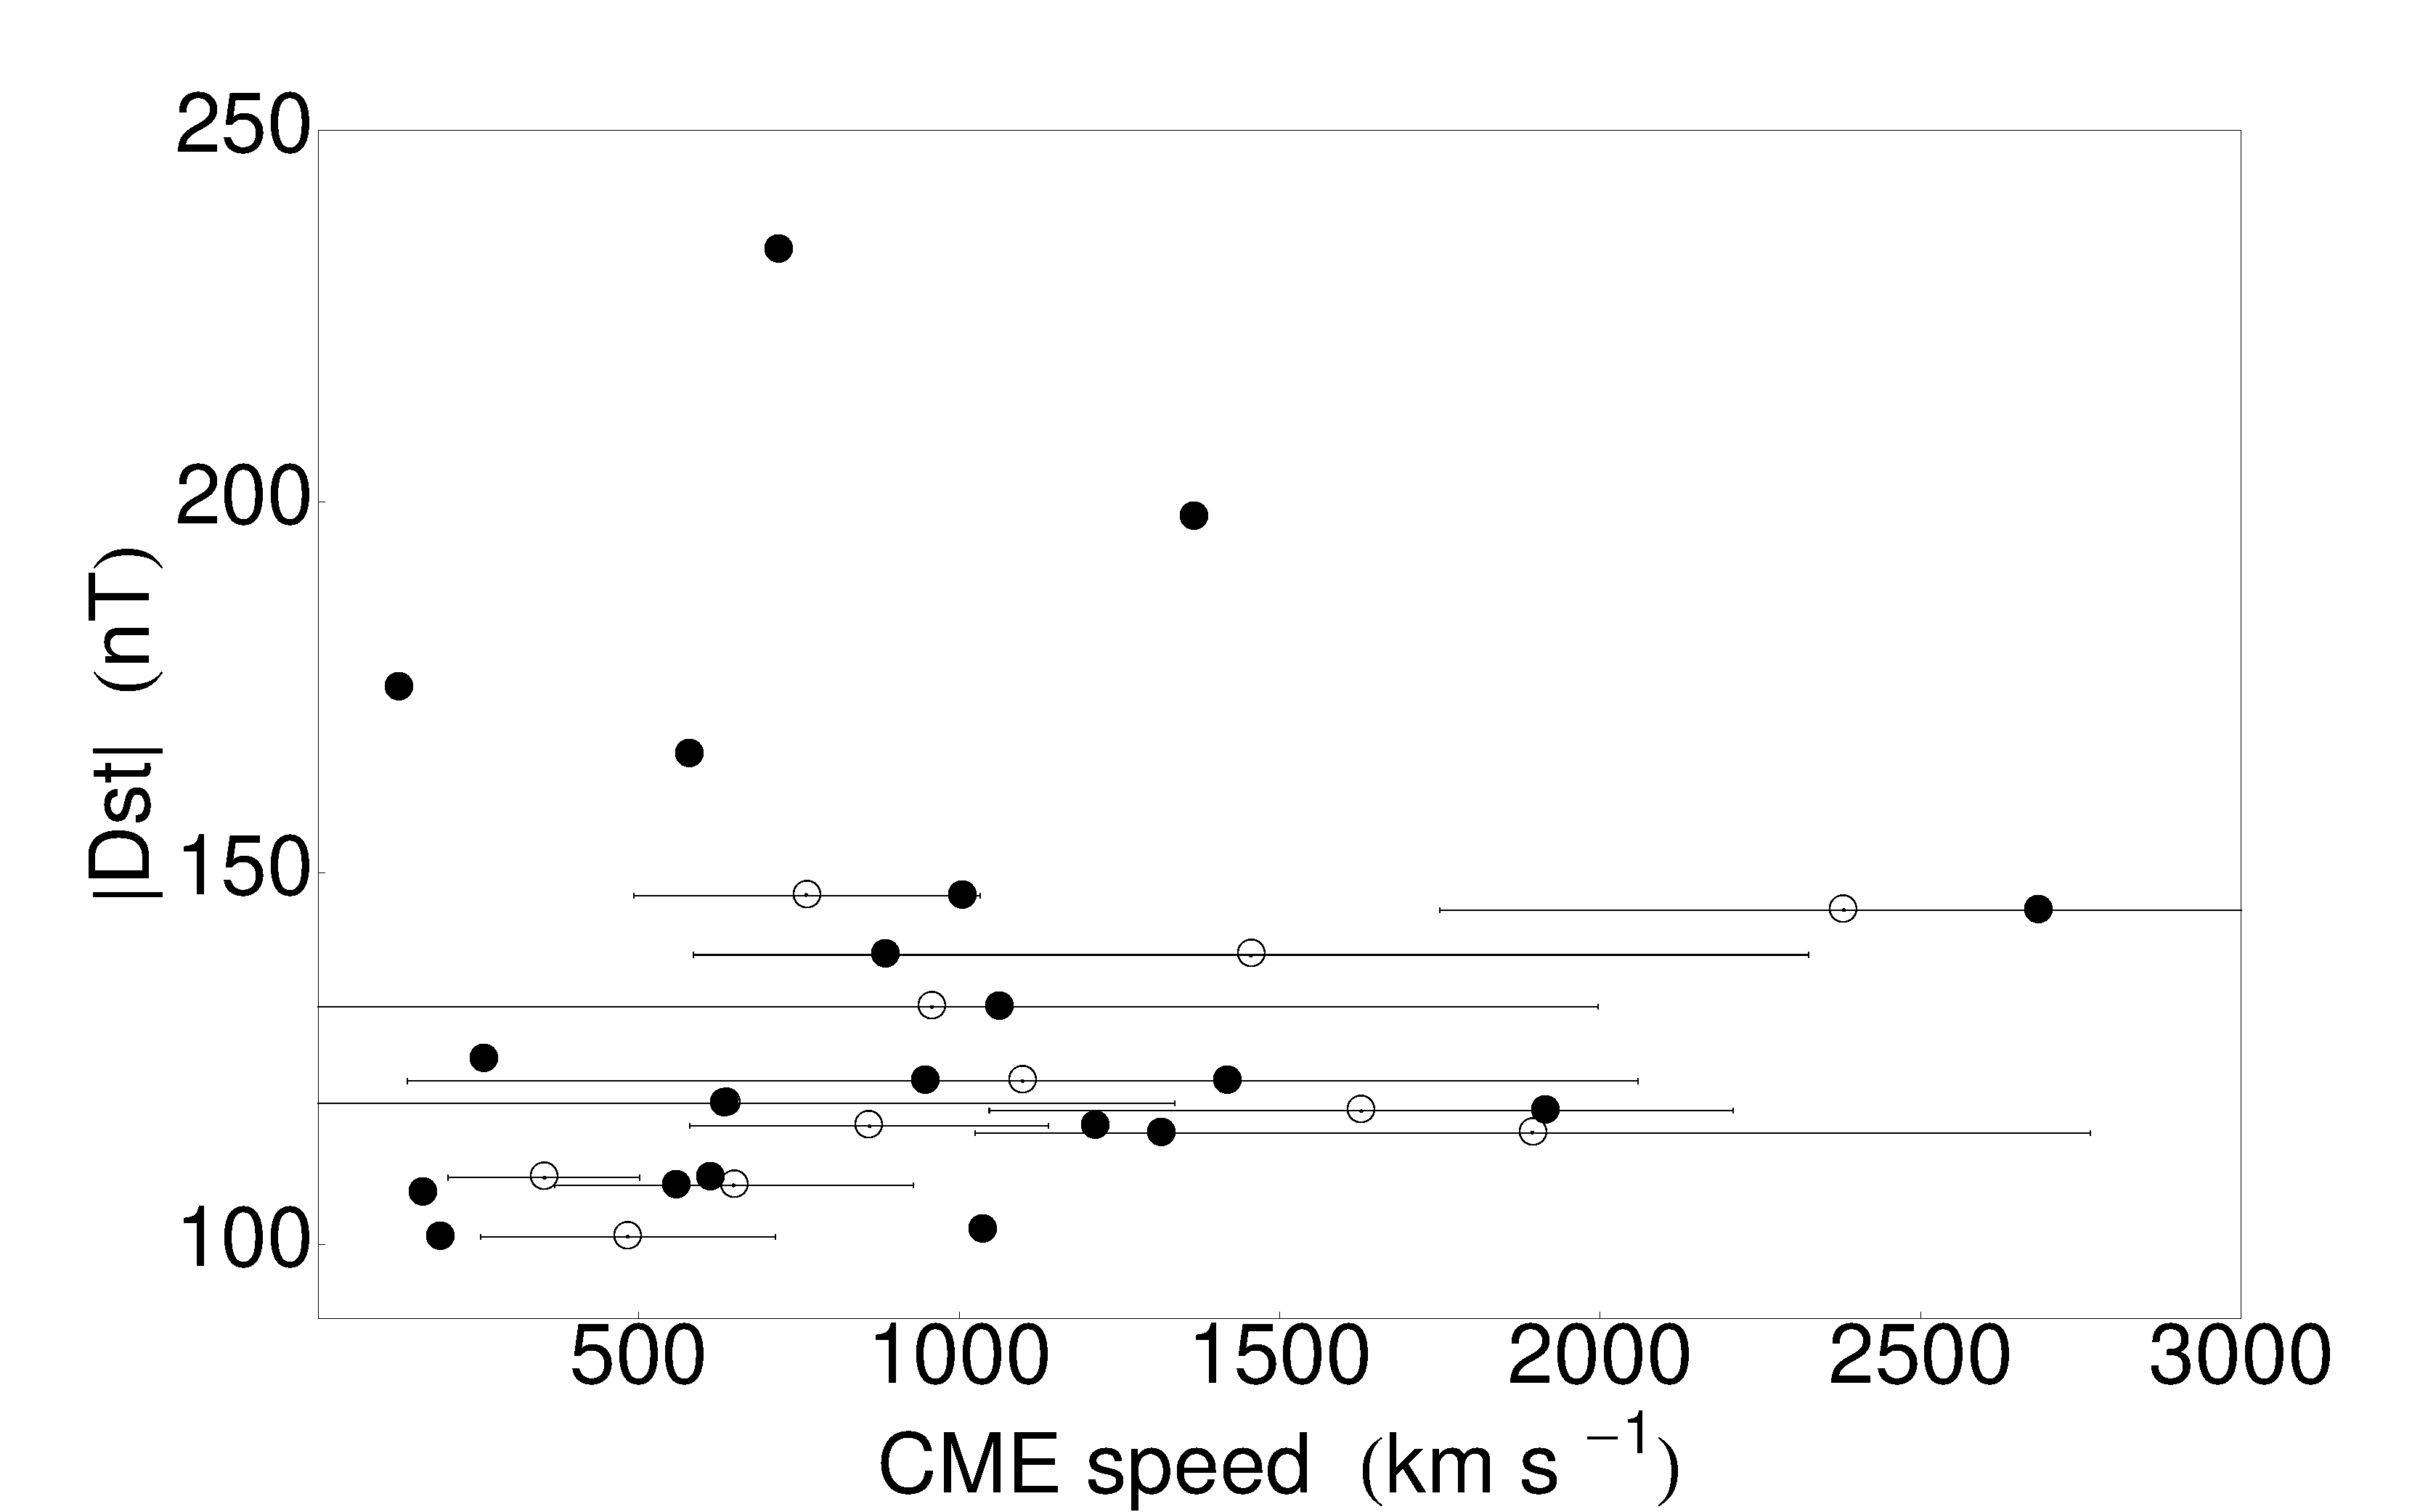
\includegraphics[width=0.7\hsize]{chapter2/figs/Fig_GS_speed_er_mean.pdf}
	\caption{Scatter plot illustrating the relationship between the Dst index and CME speed, incorporating data from the SOHO/LASCO instrument (represented by filled circles) and 3D de-projections (depicted by empty circles). Credit goes to \citet{miteva_2023}.}
	\label{fig_speeds_dst}
\end{figure}

\begin{figure}[!htp]
	\centering
	\begin{subfigure}[b]{0.45\textwidth}
		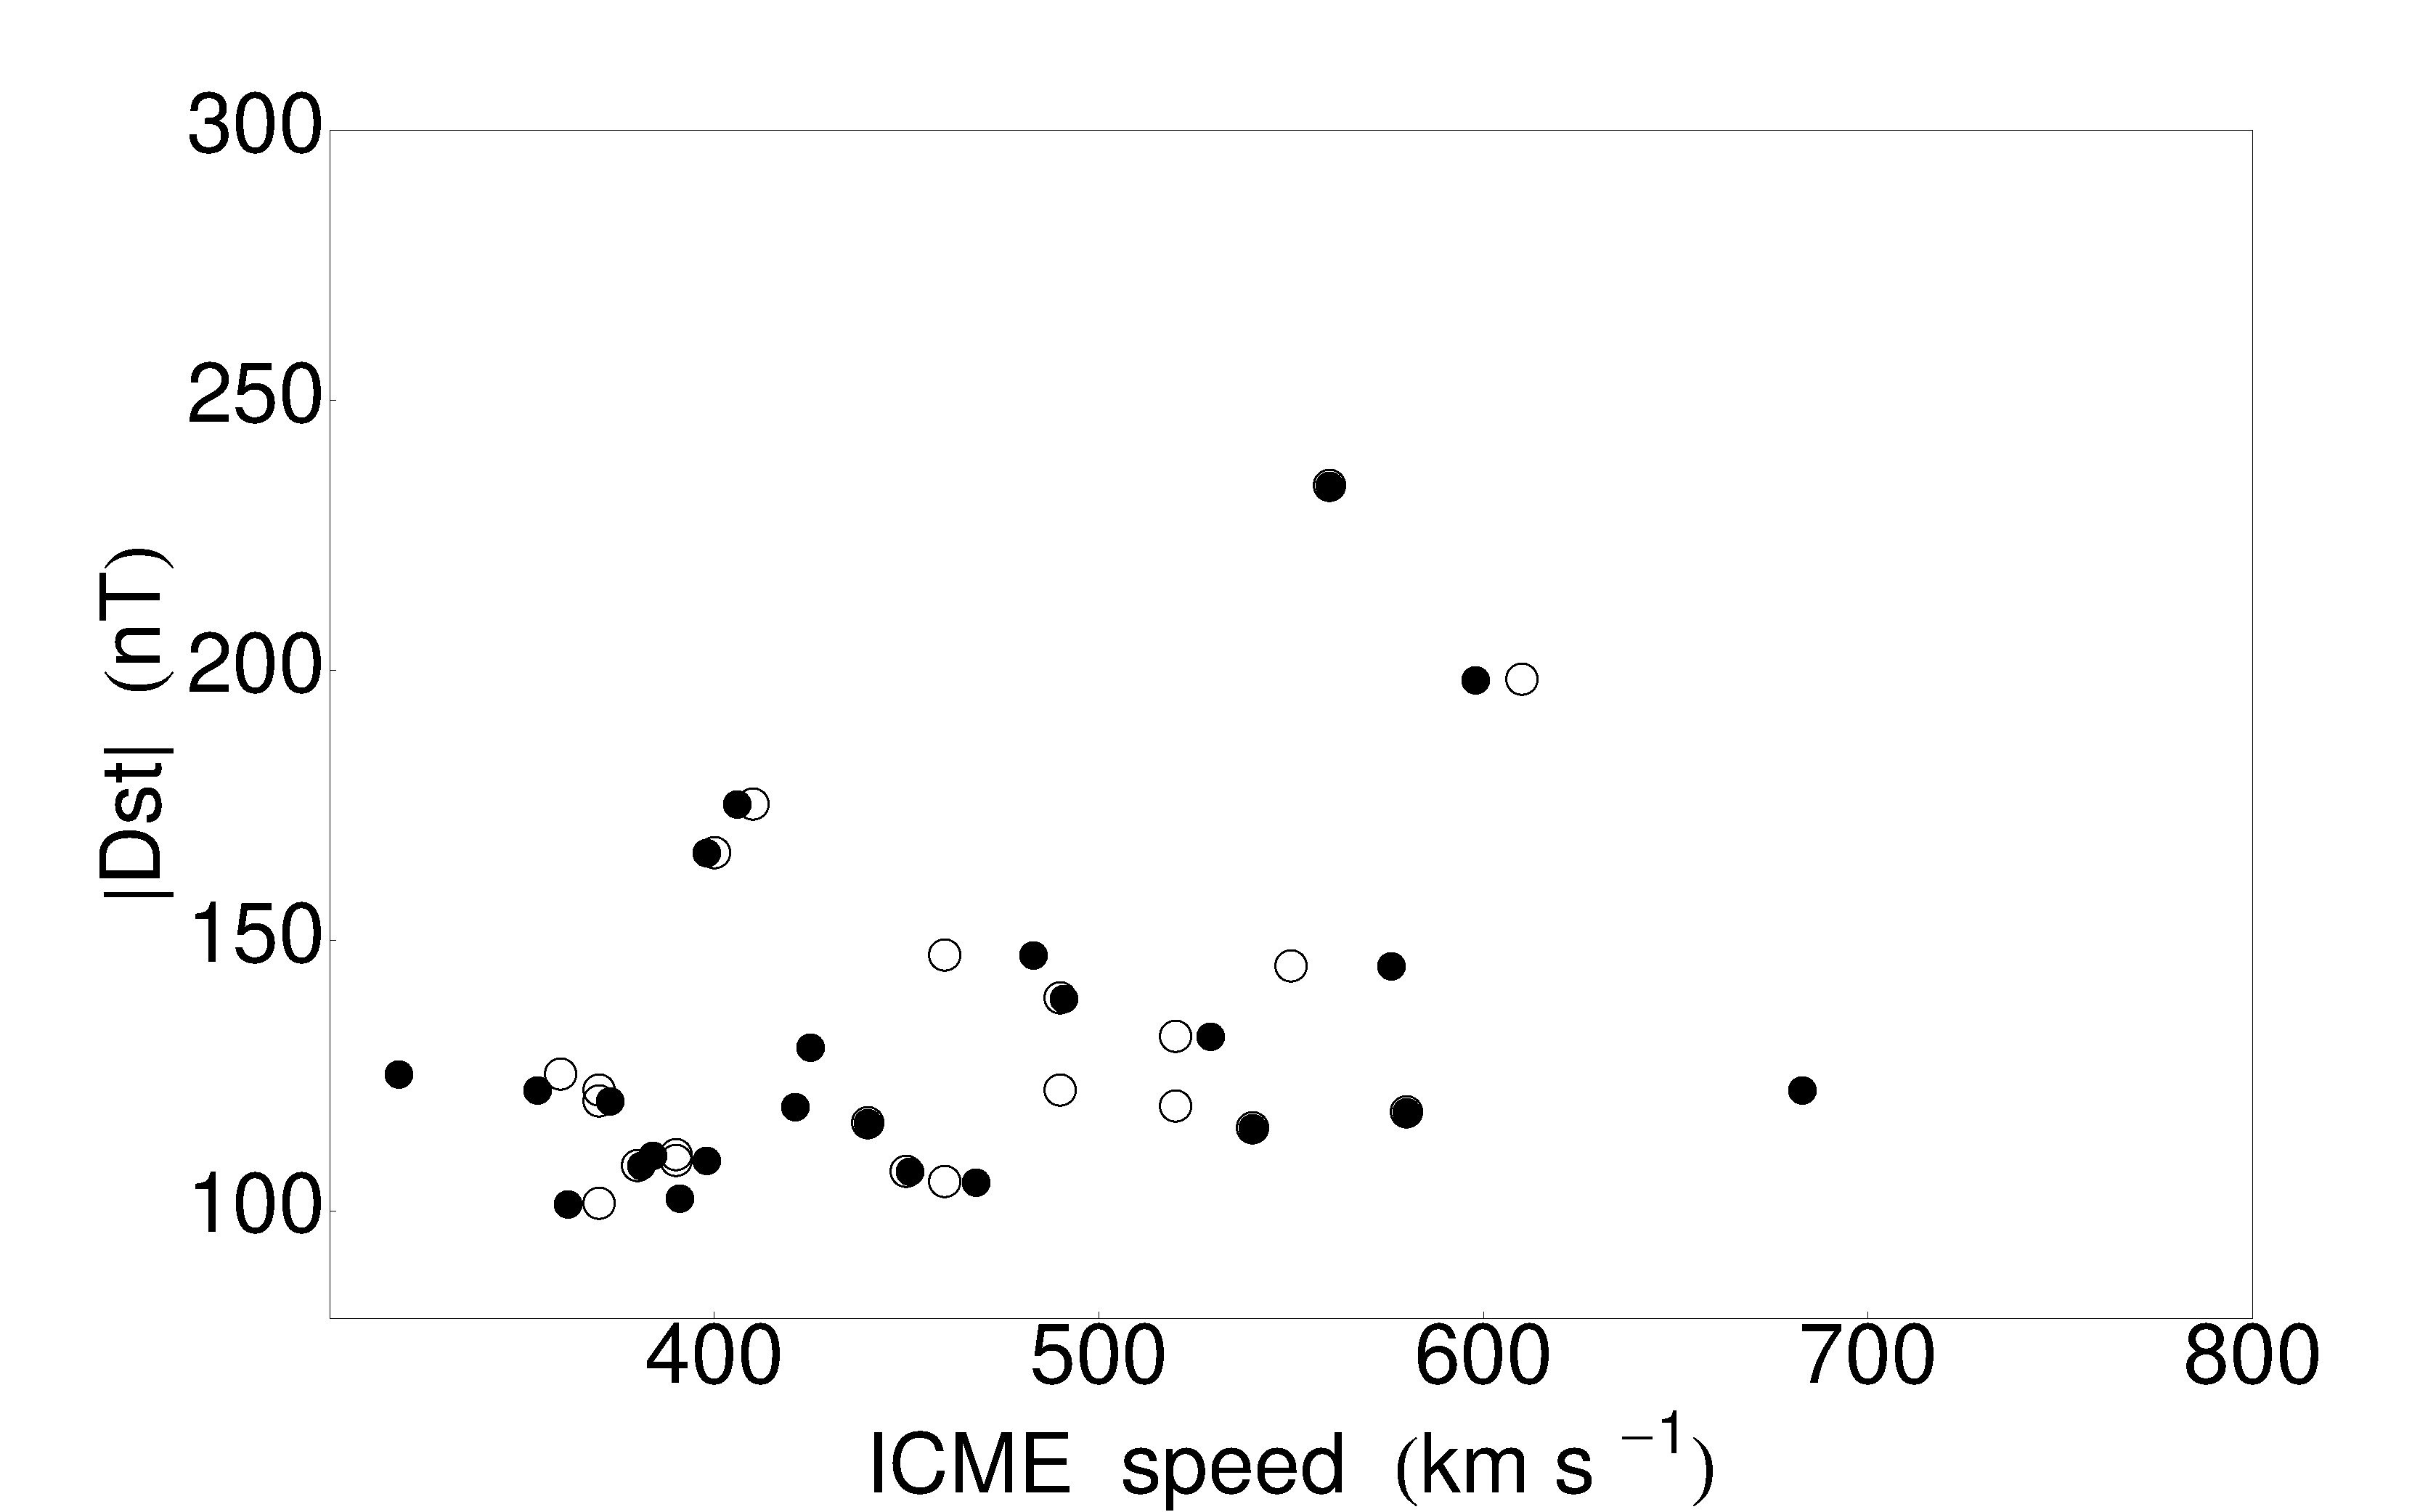
\includegraphics[width=\textwidth]{chapter2/figs/Fig_GS_ICMEspeed.pdf}
	\end{subfigure}
	\hfill
	\begin{subfigure}[b]{0.45\textwidth}
		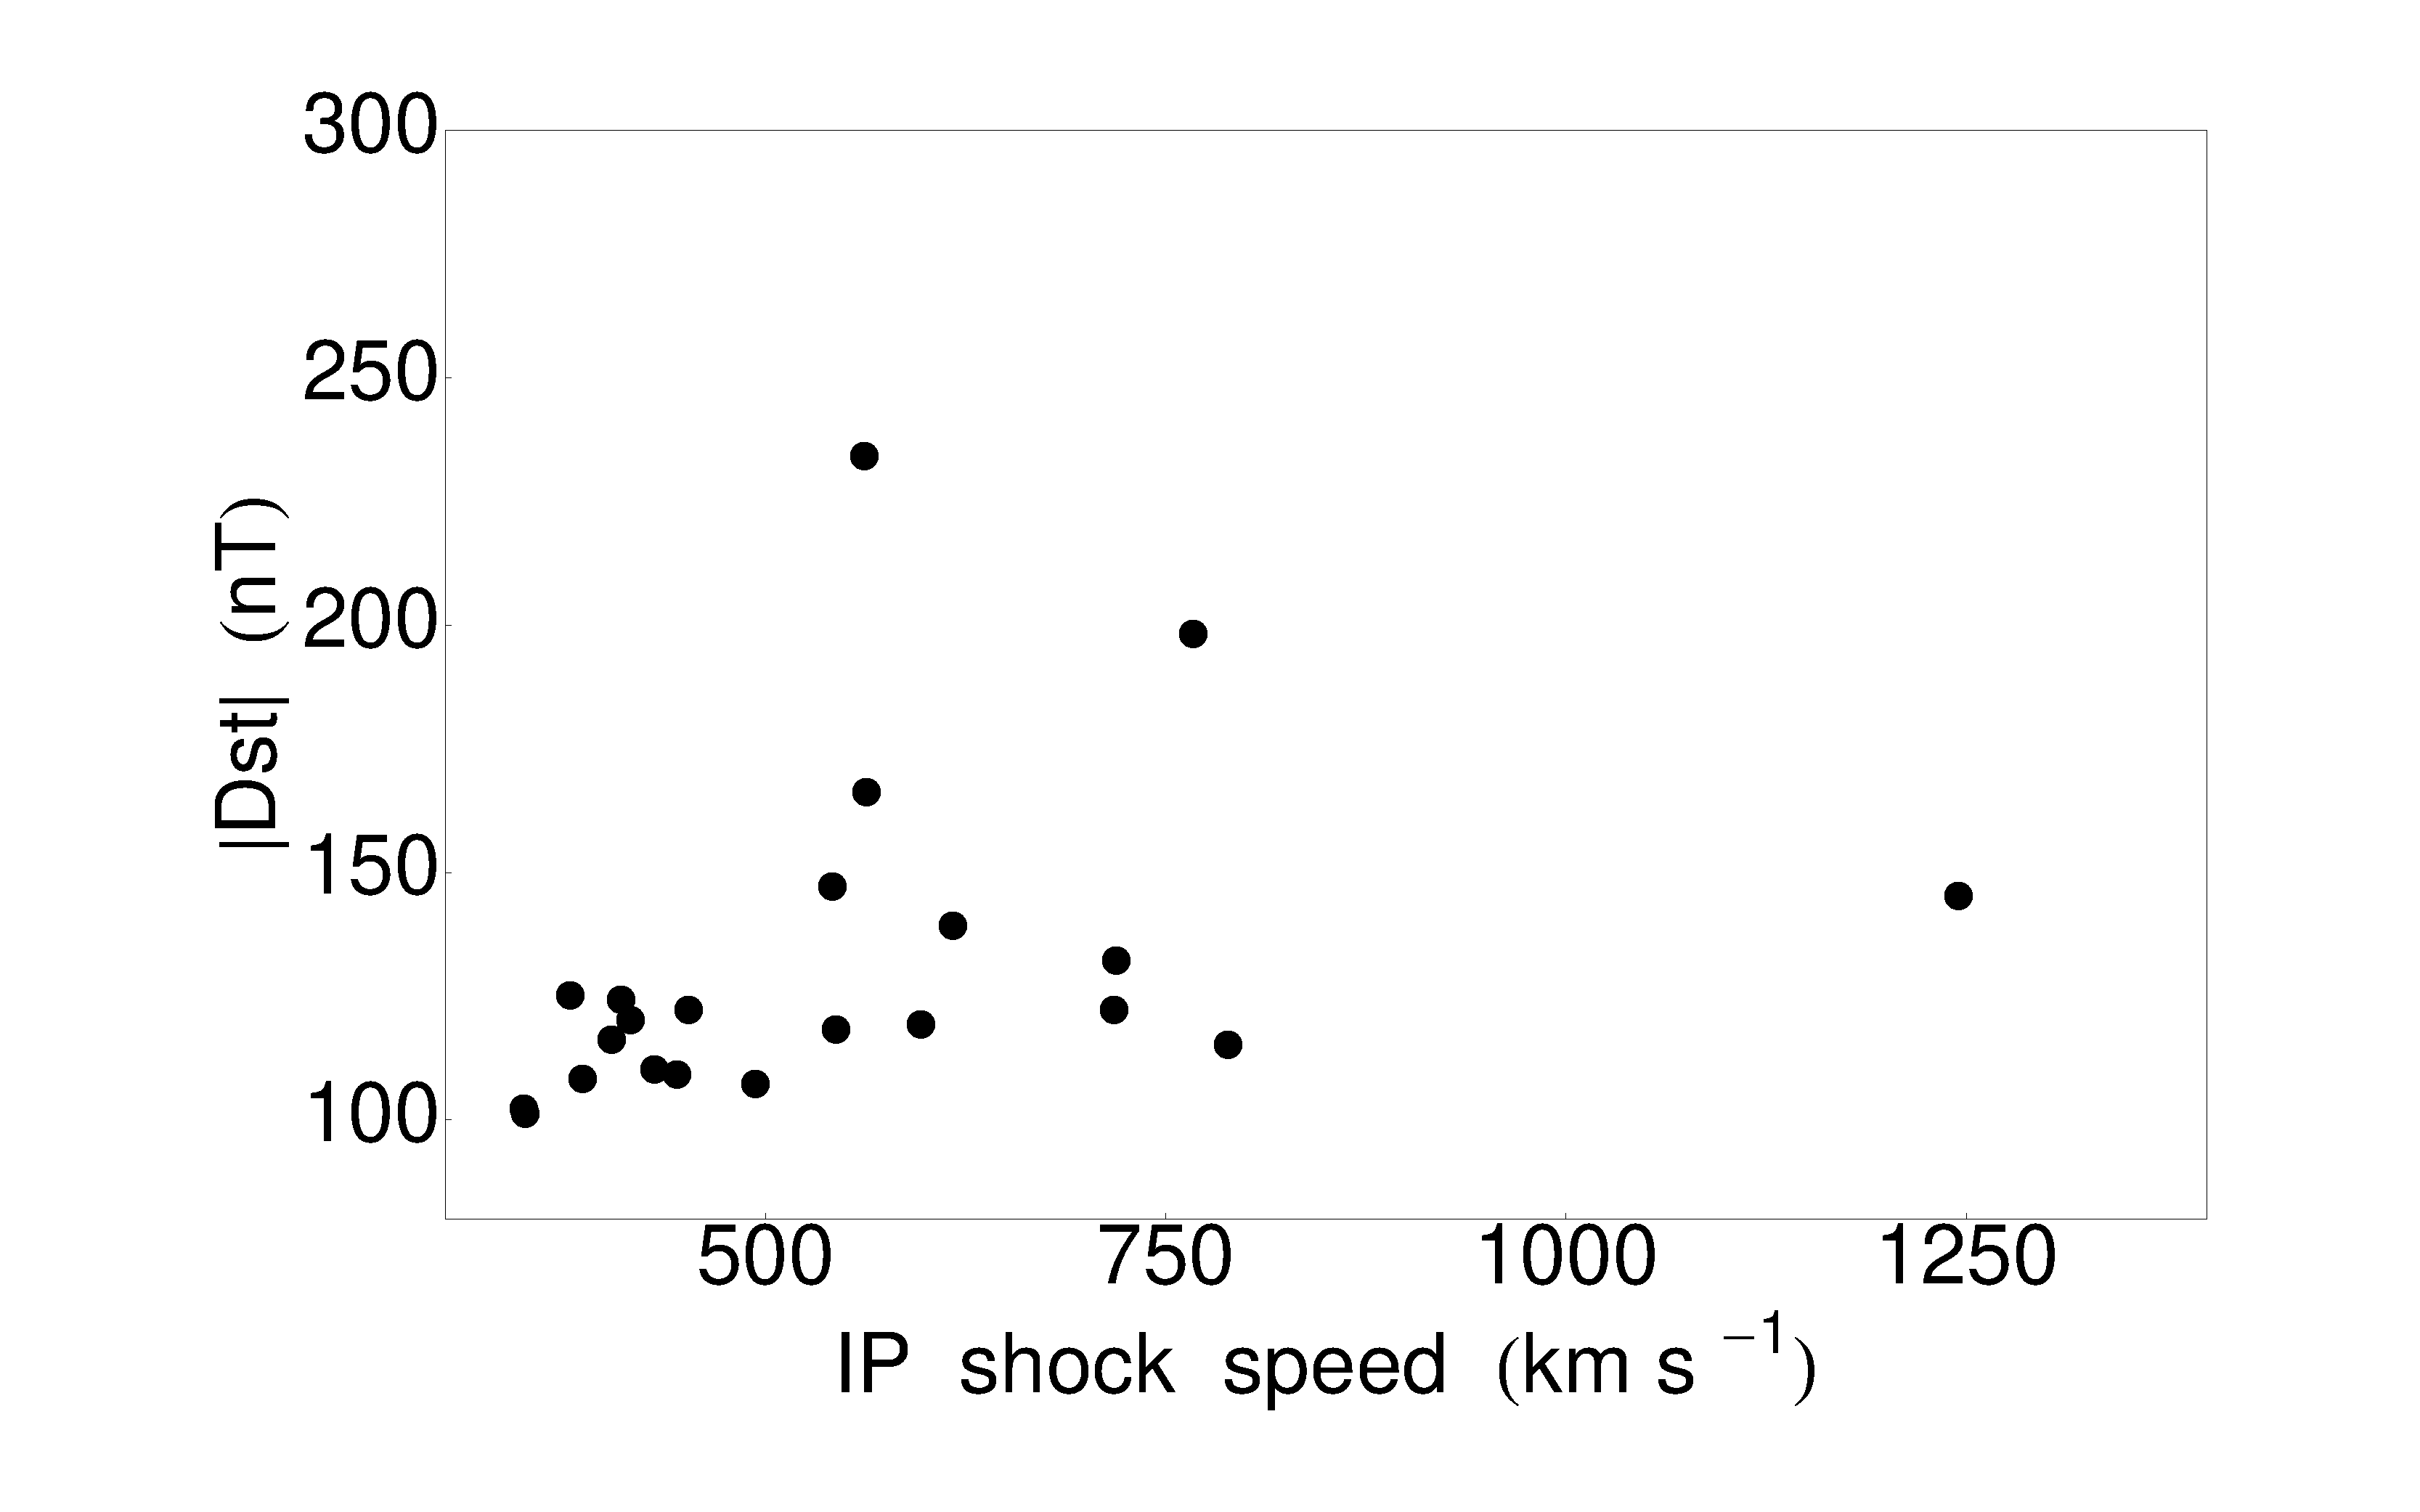
\includegraphics[width=\textwidth]{chapter2/figs/Fig_GS_IPspeed.pdf}
	\end{subfigure}
	\begin{subfigure}[b]{0.45\textwidth}
		\includegraphics[width=\textwidth]{chapter2/figs/Fig_GS_Ms.pdf}
	\end{subfigure}
	\hfill
	\begin{subfigure}[b]{0.45\textwidth}
		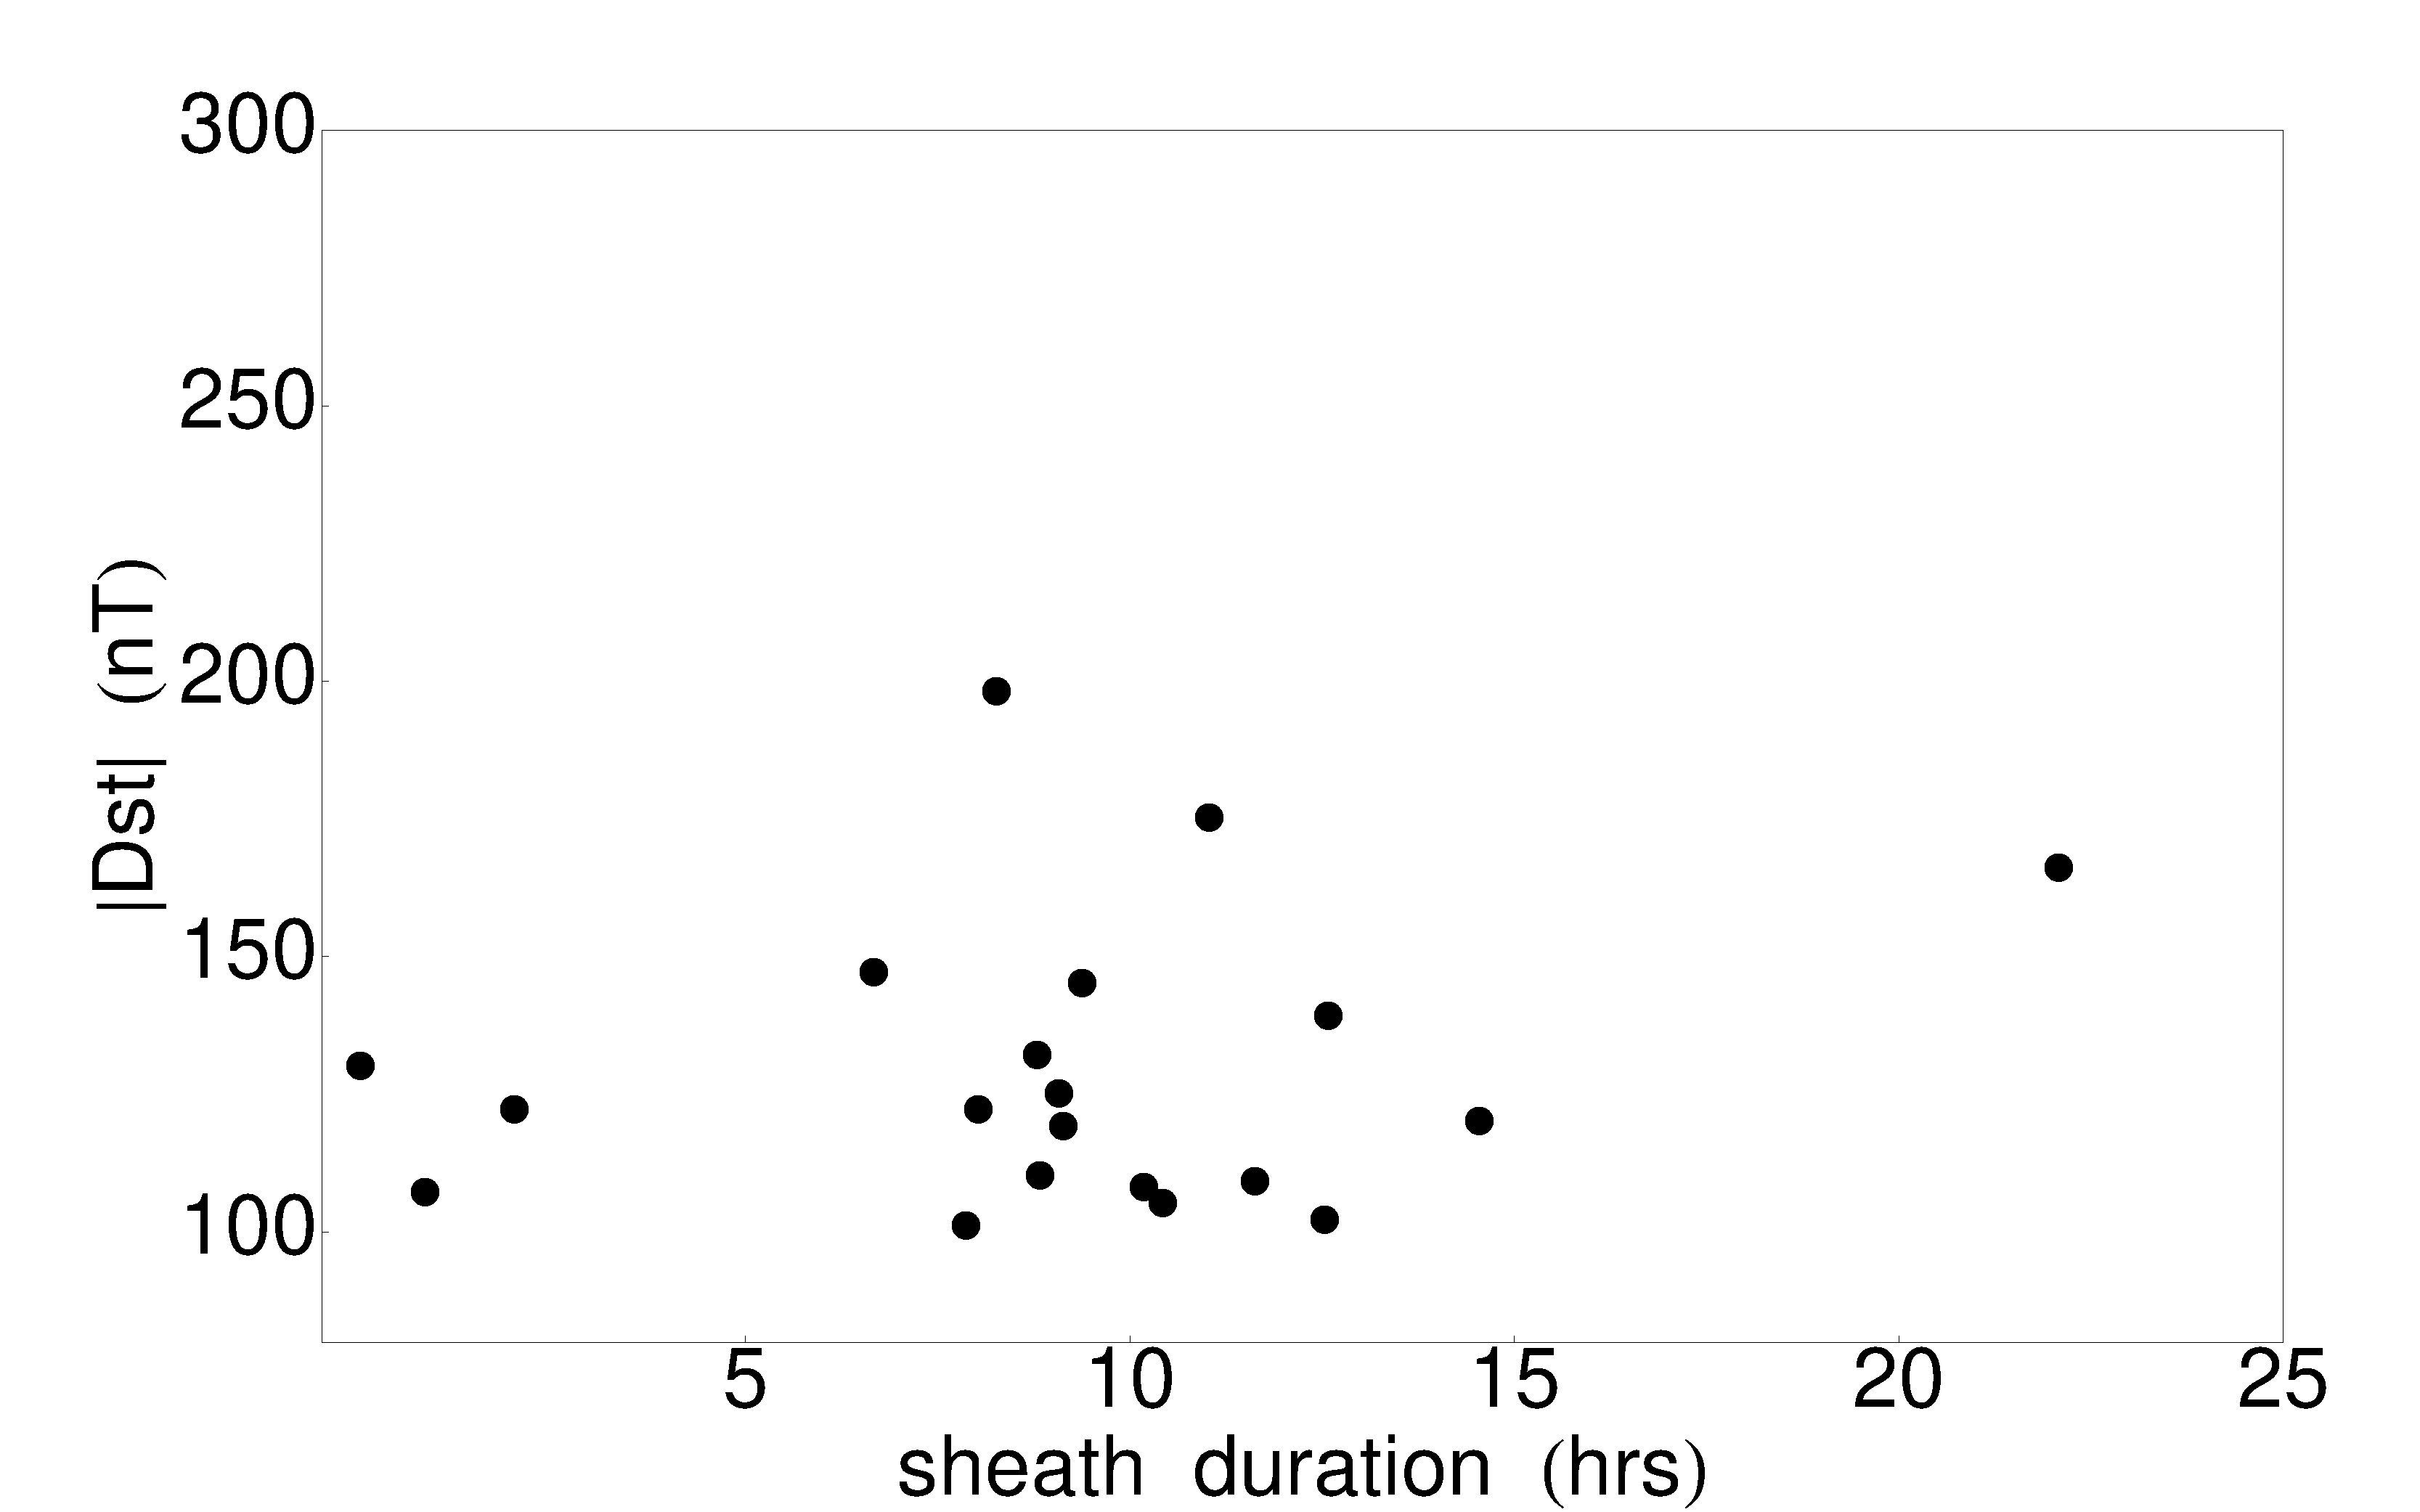
\includegraphics[width=\textwidth]{chapter2/figs/Fig_GS_sheath.pdf}
	\end{subfigure}
	\begin{subfigure}[b]{0.45\textwidth}
		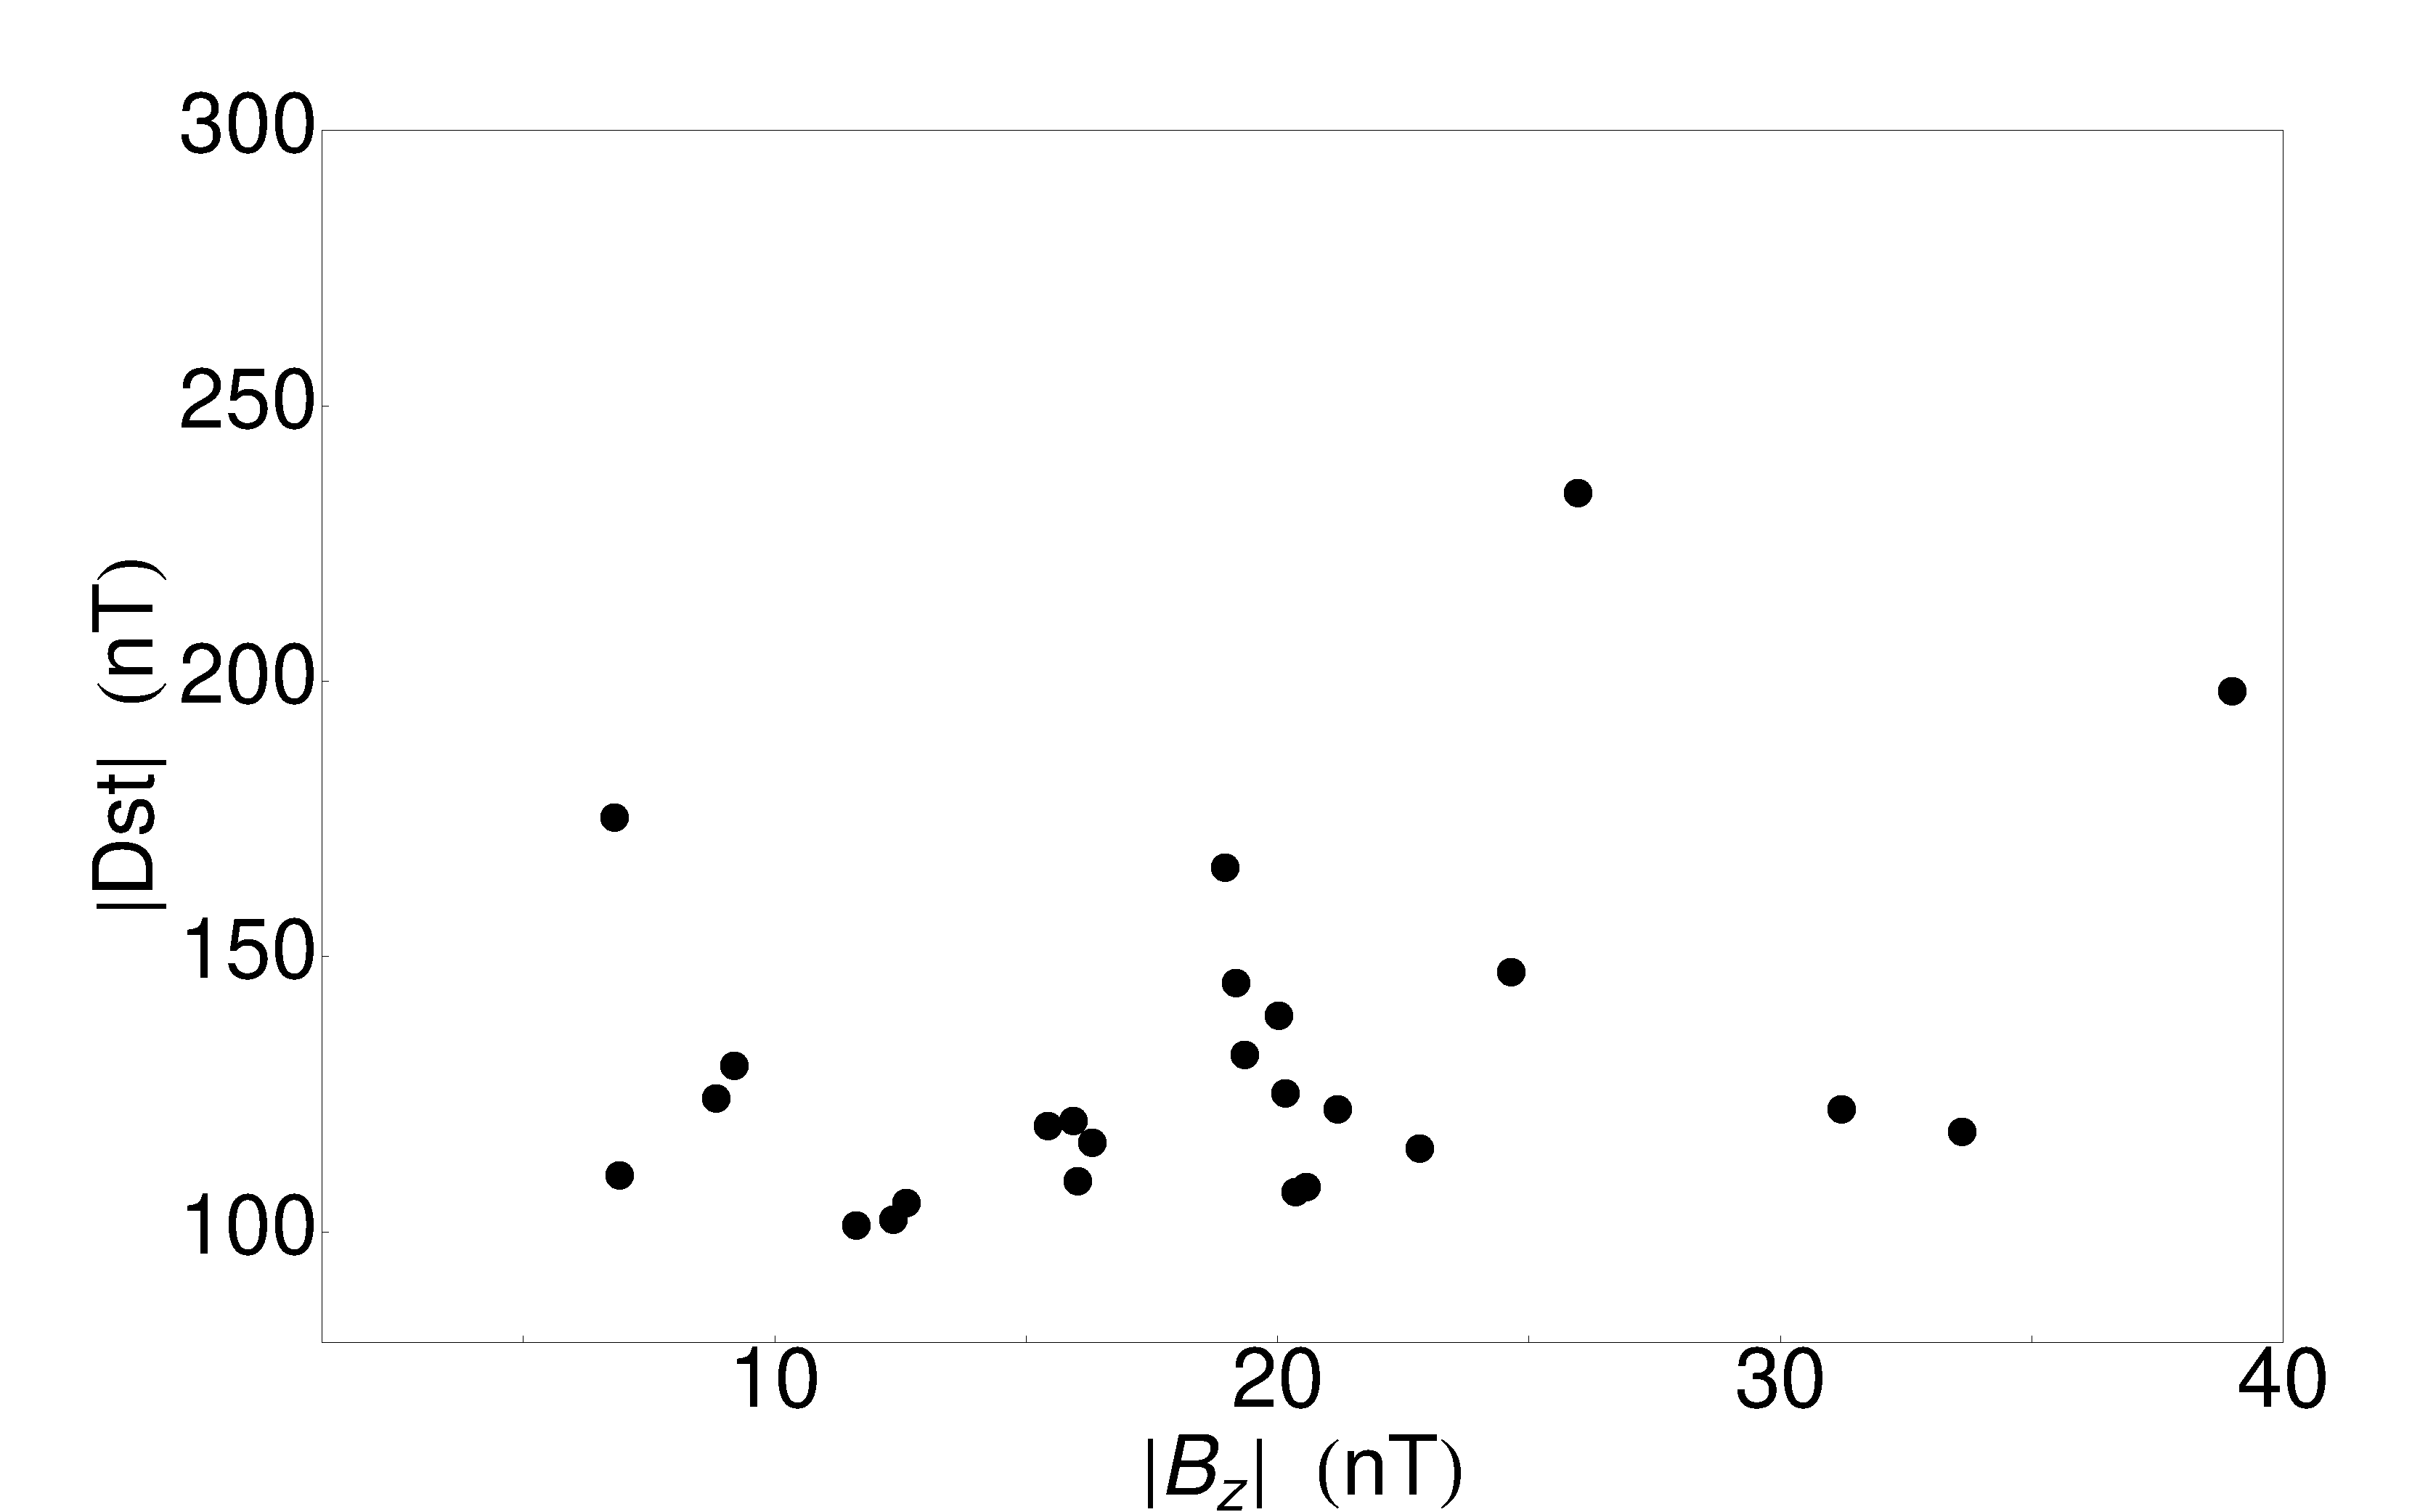
\includegraphics[width=\textwidth]{chapter2/figs/Fig_GS_Bz.pdf}
	\end{subfigure}
	\hfill
	\begin{subfigure}[b]{0.45\textwidth}
		\includegraphics[width=\textwidth]{chapter2/figs/Fig_GS_Bjump.pdf}
	\end{subfigure}
	\begin{subfigure}[b]{0.45\textwidth}
	\includegraphics[width=\textwidth]{chapter2/figs/Fig_GS_Tjump.pdf}
\end{subfigure}
	\hfill
\begin{subfigure}[b]{0.45\textwidth}
	\includegraphics[width=\textwidth]{chapter2/figs/Fig_GS_Njump.pdf}
\end{subfigure}
	\caption{Comprehensive scatter plots illustrating the relationships between Dst index and various solar wind parameters, including Wind/ACE ICME speed, IP shock speed, Mach number, duration of sheath region, Bz, magnetic field jump, temperature jump, and density jump. Credit goes to \citet{miteva_2023}.}
	\label{fig_dst_scatterplots}
\end{figure}

\begin{table}[!htp] 
	\small
	\centering
	\caption{Tabular representation of Pearson correlation coefficients between the GS Dst index and various parameters of IP phenomena. The data is derived from Wind satellite measurements, unless otherwise stated, with the corresponding sample sizes indicated in parentheses. Credit goes to \citet{miteva_2023}.}
	\label{tab_cc_IP}
	\begin{tabular}{lc}
		\toprule
		\textbf{IP parameter} & \textbf{Dst$-$IP parameter} \\
		\midrule
		ICME speed  & 0.37 (24)	\\
		ICME speed (ACE)   & 0.44 (22)	\\
		IP shock speed  & 0.35 (22)	\\
		Mach number  & 0.36 (21)	\\ 
		sheath duration & 0.22 (20) \\
		$|B_z|$      & 0.37 (25) \\
		$B_d/B_u$  & 0.48 (21)	\\
		$T_d/T_u$  & 0.40 (21)	\\
		$N_d/N_u$  & 0.46 (21)	\\
		{\bf $B$}  & {\bf $-$0.14 (20)}  \\
		{\bf $V$}       & {\bf 0.19 (20)}	\\
		{\bf $\beta_u$} & {\bf $-$0.14 (21)}	\\
		\bottomrule
	\end{tabular}
\end{table}

\subsubsection{Correlation between GSs and IP Parameters}
Here, we explore the correlations between GSs and various parameters associated with pre-selected IP phenomena. To visually represent these relationships, scatter plots are employed for specific parameter pairs. These parameters include Dst index versus ICME speed and IP shock speed, Dst versus Mach number and sheath duration, Dst versus $|Bz|$ and $B_d/B_u$, Dst versus $T_d/T_u$ and $N_d/N_u$. Figure~\ref{fig_dst_scatterplots} shows these relationships, and the corresponding Pearson correlation values elucidating these trends are documented in Table~\ref{tab_cc_IP}.

For the limited sample of GS storms utilized in our analyses, we observe a moderately positive trend between the Dst index and the plasma compression parameters at the shock interface (downstream to upstream ratio). Interestingly, these correlations are comparable to, or slightly larger than, those obtained when considering ICME speeds from the Wind and ACE spacecraft. Notably, the trend with $|Bz|$ is weaker (0.37 for our dataset), in contrast to the robust trend reported in previous studies. Furthermore, the correlations involving Dst and IP shock speed, Mach number, or sheath duration are relatively smaller.

Recent reports have highlighted strong correlations with different components of the electric and magnetic fields \citep{echer_2022}, although this aspect exceeds the scope of our current analyses. It is essential to exercise caution in interpreting these results, given the absence of uncertainty estimates for the correlation coefficients.
The ICME and IP shock catalogs employed in our study offer additional parameters, including averaged magnetic field B, plasma speed V inside the magnetic structure, and upstream plasma beta bu (not presented in Table~\ref{tab_GS_IP}). However, no robust correlations emerge between these parameters and the Dst index, with all correlation coefficients found being smaller than 0.2.

\subsubsection{On the GS Strength Forecasting Based on Solar and IP Parameters}
We examine the collective impact of magnetic obstacle type and orientation upon Earth arrival (columns 5 and 9 from Table~\ref{tab_GS_IP}), along with the 3D reconstructed CME speeds (columns 10–12 from Table~\ref{tab_GS_sol}), on the intensity of GSs, approximated in this study using the Dst index.

The most potent GSs in our compilation, arranged in descending order based on their Dst values (nT), exhibit distinctive magnetic structure parameters, including complexity, orientation of arrival, and speed at Earth (refer to Tables~\ref{tab_GS_IP} and~\ref{tab_GS_sol}):

\begin{itemize}
	\item E15 (-234): Magnetic obstacle type undefined, fast speed (f), no 3D speed estimation;
	\item E16 (-198): Complex (Cx) structure, nose-like (n) orientation, no 3D speed estimation;
	\item E25 (-175): Flux-rope (Fr) structure, nose-like (n) orientation, no 3D speed estimation;
	\item E19 (-166): Flux-rope (Fr) structure, nose-like (n) orientation, no 3D speed estimation;
	\item E03 (-147): Complex (Cx) structure, fast speed (f), reduced 3D speed compared to 2D;
	\item E04 (-145): Complex (Cx) structure, nose-like (n) orientation, similar 3D speed compared to 2D;
	\item E06 (-139): Flux-rope (Fr) structure, nose-like (n) orientation, larger 3D speed compared to 2D;
	\item E10 (-132): Flux-rope (Fr) structure, nose-like (n) orientation, similar 3D speed compared to 2D.
\end{itemize}

Upon scrutiny of these cases, it becomes apparent that the most intense GSs are linked to magnetic obstacles characterized by a nose-like (n) orientation upon arrival, coupled with either a complex (Cx) or flux-rope (Fr) structure. Exceptions include instances of fast speed flank hits or flank hits in combination with a complex (Cx) structure. It has been established that sheath duration does not serve as a decisive ordering parameter. Other GSs of lesser intensity (refer to Table~\ref{tab_GS_IP}) predominantly result from flank hits or exhibit uncertain configurations, possibly influenced by fast solar wind streams or CIRs. Notably, E20 is an exception, resulting from a nose hit; however, the IP structure associated with it has a notably low speed, as observed in the examined animations.

It is crucial to acknowledge that the IP shock speed provided by the Wind and ACE satellites represents a single point sample within the entire structure. In contrast, animations offer a global speed distribution. Therefore, our interpretation considers information from both sources — speed reconstructions and in situ measurements — to enhance the robustness of our analysis.













\section{Discussion}
%%% Nedal et al. (2023) paper
The eruption on May 11, 2011, presented a complex set of solar phenomena, including a fast partial-halo CME, a weak solar flare, an eruptive filament, and a type II radio burst. The interplay of these events and their effects on the solar and interplanetary environment provides valuable insights into the dynamic nature of solar processes.

\subsection{CME Kinematics and Coronal Shockwave Characteristics}
The CME associated with the eruption exhibited notable characteristics, such as a linear speed of 745 \kms, an acceleration of 3.3 m s$^{-2}$, and an angular width of 225\degree. The shockwave generated by the CME displayed intricate kinematics, as analyzed in both the low and middle/outer corona.

In the low corona, the shockwave was asymmetric, with differences observed in the time-dependent evolution between the left and right flanks. The aspect ratio evolution from elongation to symmetry and subsequent flattening revealed the dynamic nature of the shockwave geometry. The lateral directions exhibited differences in thickness, speed, and acceleration, indicating a complex interaction with the coronal environment. The right flank demonstrated over six times the sheath thickness observed on the left, emphasizing lateral expansion over radial propagation.

Further analysis segmented the shock surface into the Cap zone, Zone 1, and Zone 2. The shock speed at the flanks exceeded that at the Cap zone, suggesting variations in shock characteristics along its surface. The shock density jump remained consistent across the segments, indicating a relatively homogeneous magnetic structure.

In the middle/outer corona, the height-time profile of the CME leading edge provided by SOHO/LASCO measurements showcased the dynamic evolution of the EUV wave. The Gallagher model fitting captured the early stages of the event near the Sun, emphasizing the importance of a comprehensive approach in combining AIA and LASCO measurements.

The wave's rapid acceleration and subsequent speed decrease within a distance of 5\rsun from the Sun highlighted the intricate interplay between the CME and the surrounding medium. The fluctuations in acceleration and speed over time further underscored the complexity of the coronal shockwave dynamics.

\subsection{Statistical Study and Correlations}
The statistical analysis of coronal wave events in the AIA and LASCO FOVs revealed intriguing patterns. Waves in the radial direction exhibited higher speeds, acceleration, lower mean intensities, and lower thickness compared to the lateral direction, indicating early elongation near the Sun.

Cumulative dynamic spectra illustrated the decline in shock speed and intensity with increasing distance, aligning with expectations of decreasing momentum and plasma densities in the solar environment.

The investigation into plasma parameters and shock characteristics over 26 events demonstrated correlations between various pairs of parameters. Noteworthy correlations included those between the shock-field $\theta_{BN}$ angle and magnetic field amplitude, as well as between shock density jump and magnetic field magnitude.

%The scatter plot analysis highlighted strong correlations among parameter pairs, suggesting hidden connections between shock and plasma parameters.

Power fits were identified as suitable models, laying the groundwork for developing parameterizations in the subsequent phases of the project.

%%% Stepanyuk et al. (2022) paper
\subsection{Unveiling Dynamic Coronal Features with Wavetrack}
In this study, \citet{stepanyuk_2022} applied the Wavetrack methodology to investigate eruptive solar events, focusing particularly on the May 11, 2011 event associated with a prominent CBF. The analysis encompassed two additional events, occurring on June 7, 2011, and December 12, 2013, showcasing Wavetrack's versatility in tracking various solar features both on the solar disk and off the limb.

The Wavetrack algorithm efficiently delineated the evolving CBFs across consecutive time steps for the May 11, 2011 event, as depicted in Figure~\ref{fig_wavetrack_cbf_filament}. Notably, the algorithm's adaptability was evident despite variations in pixel distributions and intensities on the solar disk and near the limb. This capability allowed for a detailed exploration of the time-dependent shapes and changing intensity distributions of CBFs, distinct from the broader corona.

The segmentation of the CBF during the December 12, 2013 event underscored Wavetrack's efficacy in tracking multiple separate parts of the same feature, even under heightened coronal activity. This highlights the potential of Wavetrack as a valuable tool for studying complex solar phenomena with varying activity states.

To further probe the kinematics of CBFs and filaments, we employed the FLCT method. The results, presented in Figure~\ref{fig_flct_110511}, revealed the instantaneous plane-of-sky direction and speed of different regions within the CBF during the May 11, 2011 event. Intriguingly, the uneven expansion of the CBF from the central source was evident, with the thinnest part driven by the erupting filament exhibiting the fastest motion. This nuanced information, not discernible from intensity observations alone, underscores the complementary nature of the Wavetrack and FLCT approach in elucidating the dynamic behavior of coronal features.

\subsection{Coronal Bright Front (CBF) Kinematics}
The highest speeds observed during the event were consistently in the direction away from the Sun, above the erupting filament driver. The continued compression by the driving filament caused a thinner wavefront region and higher speeds there. The study calculated the plane-of-sky velocities of the erupting filament driver, showing that the region of highest speeds in the rising filament was directly below the region of highest speeds in the CBF.

\subsection{Geometric Centers (GC) and Centers of Mass (CM)}
The Wavetrack method provided the geometric centers and centers of mass for the May 11, 2011 event. The GC is defined as the geometric center of all Wavetrack mask pixels at a given time, while the CM includes a weighting based on the AIA 193 $\AA$ channel's base difference intensity. The study presented the kinematics of the center of mass and geometric centers for this event, showing the X-axis and Y-axis positions, radial distances, radial speeds, and the angle between the two position vectors over time.

These results provide insights into the dynamics and characteristics of the May 11, 2011 solar eruption event, highlighting the movement and speeds of key features such as the CBF and the erupting filament driver.

%%% Miteva et al. (2023) paper
\subsection{Projection Effects: The Challenge of Subjectivity in CME Speed Determination}
Our investigation into CMEs reveals a nuanced landscape marked by the inherent subjectivity in the fitting and de-projection procedures. The analysis of approximately 10 CMEs, employing three models from the PyThea framework, underscores the considerable variability in results. Two designated observers within our research team, accounting for individual considerations, conducted fitting analyses. The iterative 3D de-projection procedure led to averaged CME speeds, documented in Table~\ref{tab_fits}. The associated errors, ranging from 10\kms to twice the estimated speed, highlight the challenges and uncertainties in this process.

The observed disparities among observers, even using the same model, and the impact of different models and operating systems on results emphasize the subjective nature of visual fitting procedures. Technical limitations, such as PyThea computing resource failures and uncertainty in visual assessments, further contributed to incomplete data for specific events. Our findings echo the well-established subjectivity inherent in procedures relying on personal judgment for fit quality, aligning with the broader discussion presented by \citet{verbeke_2022}.

The averaged CME speed values, categorized by model and determined by both observers, serve as the foundation for subsequent correlation studies. Despite the challenges posed by subjectivity, these averaged values provide a basis for further analysis.

\subsection{Correlation between GSs, Coronal, and Near-Sun Parameters}
Our exploration of the correlation between GSs and various parameters, such as the GS Dst index, CME speed, and 2D LASCO CME speed, unfolds in Figure~\ref{fig_speeds_dst} and Table~\ref{tab_cc_CME}. Despite the modest sample size, the analysis reveals no discernible trend between the Dst index and CME speed, irrespective of the 3D de-projection or the 2D CME speeds. The absence of 3D speed de-projections for the most robust GSs introduces a limitation in the distribution of 3D speeds, impacting overall findings.

Pearson correlation coefficients, systematically documented in Table~\ref{tab_cc_CME}, range from negligible to moderate, indicating diverse relationships between CME speed estimations and the GS Dst index. Notably, no significant correlations are identified between the Dst index and other coronal parameters, such as SF class, location, and CME AW. The complexities in these relationships highlight the need for cautious interpretation, given the data constraints and uncertainties associated with the correlation coefficients.

\subsection{Correlation between GSs and IP Parameters}
The examination of correlations between GSs and IP parameters unfolds in scatter plots in Figure~\ref{fig_dst_scatterplots}, accompanied by Pearson correlation values in Table 5. Noteworthy trends include a moderately positive correlation between the Dst index and plasma compression parameters at the shock interface, comparable to correlations with ICME speeds. However, caution is advised in interpreting results due to the absence of uncertainty estimates for correlation coefficients.

Additional parameters from ICME and IP shock catalogs, including averaged magnetic field $B$, plasma speed $V$, and upstream plasma $\beta_u$, exhibit no robust correlations with the Dst index. The complexities in these relationships underline the multifaceted nature of GS-IP parameter associations.

\subsection{GS Strength Forecasting: Unraveling Magnetic Structures}
Our analysis of the collective impact of magnetic obstacle type, orientation, and 3D reconstructed CME speeds on Geospace Storms (GSs) sheds light on intriguing patterns. The most potent GSs, based on descending Dst values, exhibit distinctive magnetic structure parameters, such as complexity, orientation of arrival, and speed at Earth. Notably, nose-like (n) orientation, coupled with a complex (Cx) or flux-rope (Fr) structure, characterizes the most intense GSs. Exceptions include instances of fast-speed flank hits or flank hits in combination with a complex (Cx) structure.

The interplay of magnetic obstacle characteristics, orientation, and 3D CME speeds provides valuable insights into the factors influencing GS intensity. However, it is crucial to acknowledge the limitations of single-point IP shock speed measurements and the need for a comprehensive interpretation that considers both speed reconstructions and in situ measurements.

\section{Conclusions}
%%% Nedal et al. (2023) paper
I have conducted a comprehensive study focusing on the characterization of 26 historical CME-driven CBFs in the low solar corona. These events were accompanied by type III radio bursts, and SEP events near Earth and were observed by the AIA instrument onboard the SDO spacecraft in the EUV 193 $\AA$ band. To achieve this, we utilized the SPREAdFAST framework, which encompasses physics-based and data-driven models to estimate the coronal magnetic field, dynamics of coronal shock waves, energetic particle acceleration, and SEP propagation in the heliosphere.

Our analysis relied on sequences of base-difference images obtained from the AIA instrument. These images served as the primary input data for our investigation. We employed these data to generate annulus plots and J-maps to estimate the kinematic measurements in both the radial and lateral directions for the EUV waves.

In order to obtain a thorough understanding of the CBFs, we computed various time-dependent and distance-dependent kinematic parameters. These included shock speed, acceleration, intensity, and thickness of the front, peak, and back edges of the waves, as well as the major and minor axes and the rate of change of the waves' aspect ratios. To augment our analysis based on AIA observations, we incorporated LASCO measurements up to 17\rsun. This additional data is important in improving the characterization of the SEP spectra near the Sun.

The analysis of kinematic measurements played a pivotal role in our study as they enabled us to generate time-dependent 3D geometric models of wavefronts. In addition, these measurements provided valuable insights for deriving time-dependent plasma diagnostics by incorporating the outcomes of the MHD and DEM models.

To accurately represent the shocks, we employed shock kinematic measurements to fit a geometric spheroid surface model for each measured time step. This approach allowed us to capture the intricate characteristics of the shocks with precision.

In order to gain a deeper understanding of the phenomenon, we explored the parametrized relationships between the modeled plasma parameters. Through this analysis, we aimed to identify potential connections and interdependencies, shedding light on the complex dynamics at play.

Overall, our findings in this study and in \citet{kozarev_2022} as well as \citet{stepanyuk_2022} contribute to a nuanced understanding of shock kinematics and shock plasma parameters.

Moving forward, our future investigations will focus on examining SEP acceleration near the Sun, as well as investigating the transport of coronal and interplanetary particles using the insights gained from our models. Additionally, we aim to refine the methods of shock and coronal parameters characterization, which will contribute to enhancing the accuracy and reliability of the results.

%%% Stepanyuk et al. (2022) paper
In the study led by \citet{stepanyuk_2022}, we introduce Wavetrack, an innovative approach designed for the automated identification and monitoring of dynamic coronal phenomena. Employing wavelet decomposition, feature enhancement, filtering, and ultimate object recomposition, Wavetrack generates time-dependent masks for feature pixels. These masks can be applied to integral or base-difference images, yielding comprehensive feature maps. Notably, Wavetrack excels in tracing pixels associated with faint, large-scale features, such as coronal bright fronts/EUV waves in AIA observations, and has demonstrated efficacy in tracking eruptive filaments.
Operable for both on-disk and off-limb features, Wavetrack adeptly follows features that evolve into distinct components over time. Implemented as a versatile, object-oriented framework in Python, Wavetrack is freely accessible for download and utilization.

The application of Wavetrack to four distinct events, with emphasis on three – the CBFs occurring on May 11 and June 07, 2011, and December 12, 2013 – reveals its proficiency in tracking complete CBF pixel maps. These model results, when integrated with the FLCT method for calculating plane-of-sky speeds, unveil the dynamic evolution of driven and non-driven regions within CBFs, as well as their correlation with eruptive filament drivers. Our findings indicate that drivers induce a compression effect, causing CBF thinning and increased speed, aligning with theoretical models. However, the brightness of CBFs in the driven regions, as observed in AIA data, does not necessarily exhibit a significant increase.

Furthermore, Wavetrack facilitates the tracking of temporal changes in feature regions by computing the time-dependent vector between the pixel geometric center and the center of mass, determined by weighing the observed pixel intensities. This proves particularly valuable for large-scale features like CBFs, providing a straightforward metric in the form of a one-dimensional time series for characterizing feature evolution.

While the method demonstrates widespread applicability to various solar dynamic features and observational data, it currently relies on human input for the segmentation of specific feature types, particularly dim ones. Manual setting of object criteria, including threshold intervals and recomposition weight coefficients, is necessary. In instances of base difference imaging, precise selection of the base image is crucial to prevent contamination of input data with spurious features. Additionally, parameter fine-tuning through trial and error may be required for specific events. These limitations are acknowledged, and future work will address them to enhance the model's versatility.

The methodology holds promise for extensive application across diverse solar dynamic features and observational datasets. Subsequent research endeavors will extend its use to in-depth studies of filament evolution and coronagraph data. The objective is to refine our comprehension of how large-scale eruptive fronts manifest variations across distinct observational contexts, spanning the low and middle corona.

%%% Miteva et al. (2023) paper
In the study led by \citet{miteva_2023}, we conduct post-event analyses of all geo-effective storms observed during solar cycle 24 with the aim of identifying distinct and reliable predictors for GS intensity. The overarching objective is to derive dependable solar or near-Sun parameters from remote sensing image data that can be effectively utilized for early warnings regarding potential GS onsets and their strength. Our approach involves the integration of solar, near-Sun, and interplanetary parameters, primarily sourced from catalogs but also subject to our analysis using space-related databases. Notably, we incorporate the results obtained from a novel tool for CME speed de-projection, termed PyThea, which is employed for the first time alongside well-established parameters in space weather and geophysics research.

Among the solar and near-Sun phenomena considered, certain selected parameters exhibit a positive correlation with the Dst index. Notably, the correlation coefficient, when comparing the observed projected CME speed, experiences an improvement from 0.04 (as obtained from LASCO) to a range of 0.34–0.55, achieved through various geometrical models provided by the PyThea software package, combining LASCO and STEREO data. However, our exploration of different CME geometry reconstruction techniques reveals a susceptibility to large speed errors, particularly in the case of fast CMEs. This aligns with findings from prior studies focusing on CME arrival time and speed forecasts for Earth, suggesting a potential overestimation of CME launch speed for fast events, likely attributable to the increased complexity in discerning coronal structures due to the rapid expansion of the magnetic structure associated with the CME.

Moreover, our examination indicates that fast halo CMEs may exhibit significant deviations, stemming from the overlap in shock and magnetic structure components, thereby strongly impacting the reconstruction quality. Consequently, we assert that the derived near-Sun 3D parameters continue to possess limited forecasting potential for predicting GS strength. In contrast, most selected IP parameters derived from in situ measurements display moderate positive correlations with GS strength, in line with expectations. However, the Bz parameter (southward component of the magnetic field) shows a relatively low correlation coefficient of 0.37, possibly influenced by the limited event sample used in our study.

Other IP parameters, such as ICME and IP shock speeds, along with their derivative parameters (e.g., Mach number), exhibit a positive trend with the Dst index, featuring correlation coefficients of 0.35–0.45. Nevertheless, none of these parameters emerge as predominant, and their reliance on single-point in situ observation raises considerations about their comprehensive predictive capability. Discrepancies in ICME speed values between ACE and Wind measurements prompt further investigation, with slightly stronger correlation coefficients (0.4–0.5) observed when utilizing different shock parameters. However, averaged values of magnetic field and speed within the magnetic structure, plasma beta in the upstream region, or duration of the sheath region show no correlation with GS strength.

Among the multitude of considered solar, near-Sun, and IP parameters, only the combination of speed and orientation (nose-like) of the magnetic obstacle appears to exert a positive influence on GS strength, as indicated by qualitative results obtained from animations accessible at \textit{helioweather}. Consistent with earlier studies, de-projected CME speeds emerge as imperative for enhancing modeling accuracy when predicting CME propagation through the IP space. However, a notable observation is the apparent lack of direct impact of 3D de-projected CME speed on GS intensity. Consequently, an accurate estimation of the ICME speed distribution over the entire ICME structure upon arrival at Earth assumes significant importance. We emphasize the imperative need for permanent stereoscopic observations, exemplified by the upcoming ESA Vigil mission situated at Lagrange point L5. Future research endeavors should aim for a more comprehensive disentanglement of distinct CME structures, thereby enabling more reliable 3D reconstructions of CME geometries for a nuanced estimation of 3D speed and directivity.

%%% Total
% Mohamed
The identified correlations and statistical patterns provide a foundation for the ongoing project. Further work will focus on refining parameterizations and establishing synoptic MHD parameters corresponding to measured shock parameters. The ultimate goal is to enhance the representation of shock parameters in the \textit{S3M} synoptic model, contributing to a more comprehensive understanding of solar dynamics and space weather forecasting.

% Oleg
Our findings emphasize the significance of integrating advanced tracking methodologies like Wavetrack with kinematic analyses such as FLCT. This synergistic approach enables a more comprehensive understanding of the intricate dynamics involved in eruptive solar events, shedding light on the complexities of CBF evolution and its correlation with eruptive features. As we continue to refine and expand such methodologies, our ability to decipher the underlying mechanisms governing solar phenomena will undoubtedly advance, contributing to the broader field of Heliophysics.

% Rosi
In conclusion, our findings underscore the complexity and subjectivity inherent in studying CMEs and their impact on Geospace Storms. The integration of observational data, model outputs, and correlation analyses offers a comprehensive perspective, laying the groundwork for further investigations into the dynamic interplay between solar and interplanetary phenomena in shaping space weather events.
